\section{Model dependence for UniFold}
\label{sec:stresscunifolddet}

Figures~\ref{fig:stressc_pT_trackj1},~\ref{fig:stressc_tau1_trackj1}, and~\ref{fig:stressc_y_trackj1} show further examples of the deterministic weight stress test for UniFold, continuing from Sec.~\ref{sec:modeldep}.

\begin{figure}[h!]
\centering
\subfloat[Input histograms]{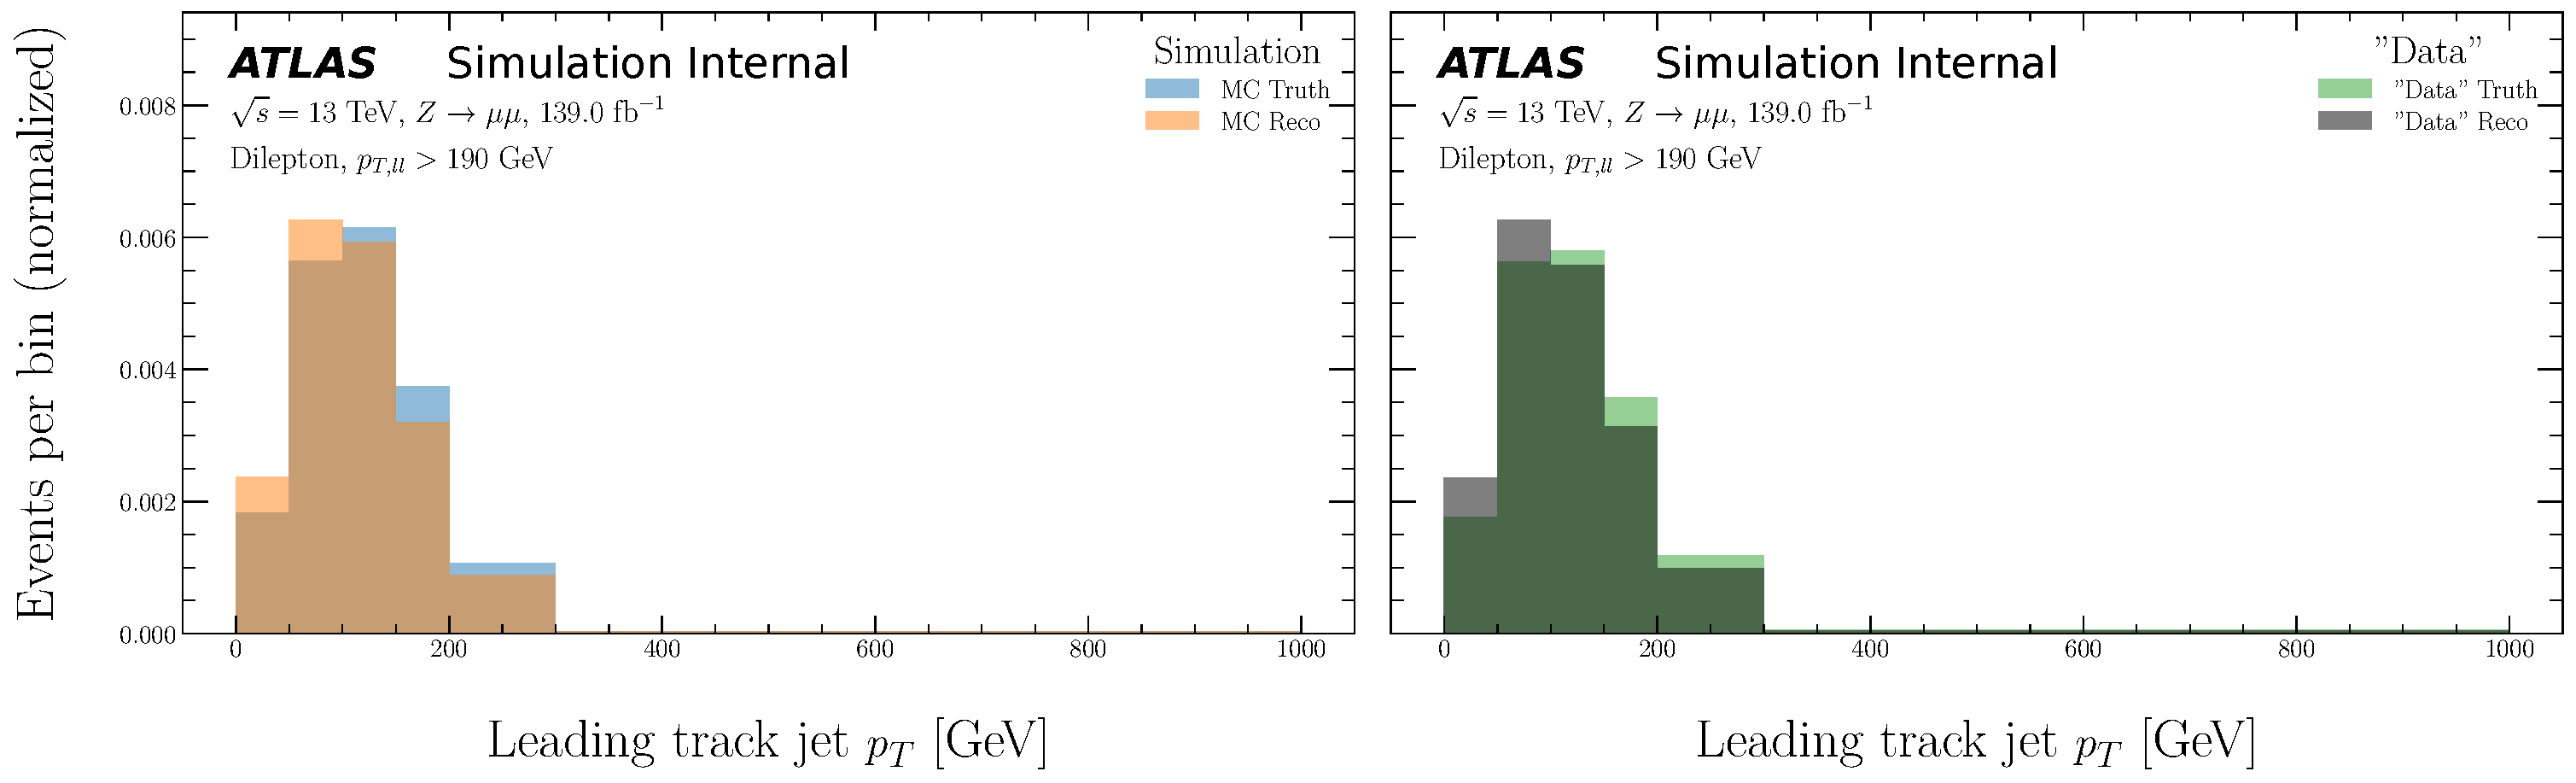
\includegraphics[width=0.85\textwidth]{figures/ATLASOmniFold-StressTest/ATLASOmniFold-StressTestC/UniFold/pT_trackj1/ATLASOmniFold-StressTestC-UniFold-pT_trackj1-Distributions}}\\
\subfloat[After 1 iteration]{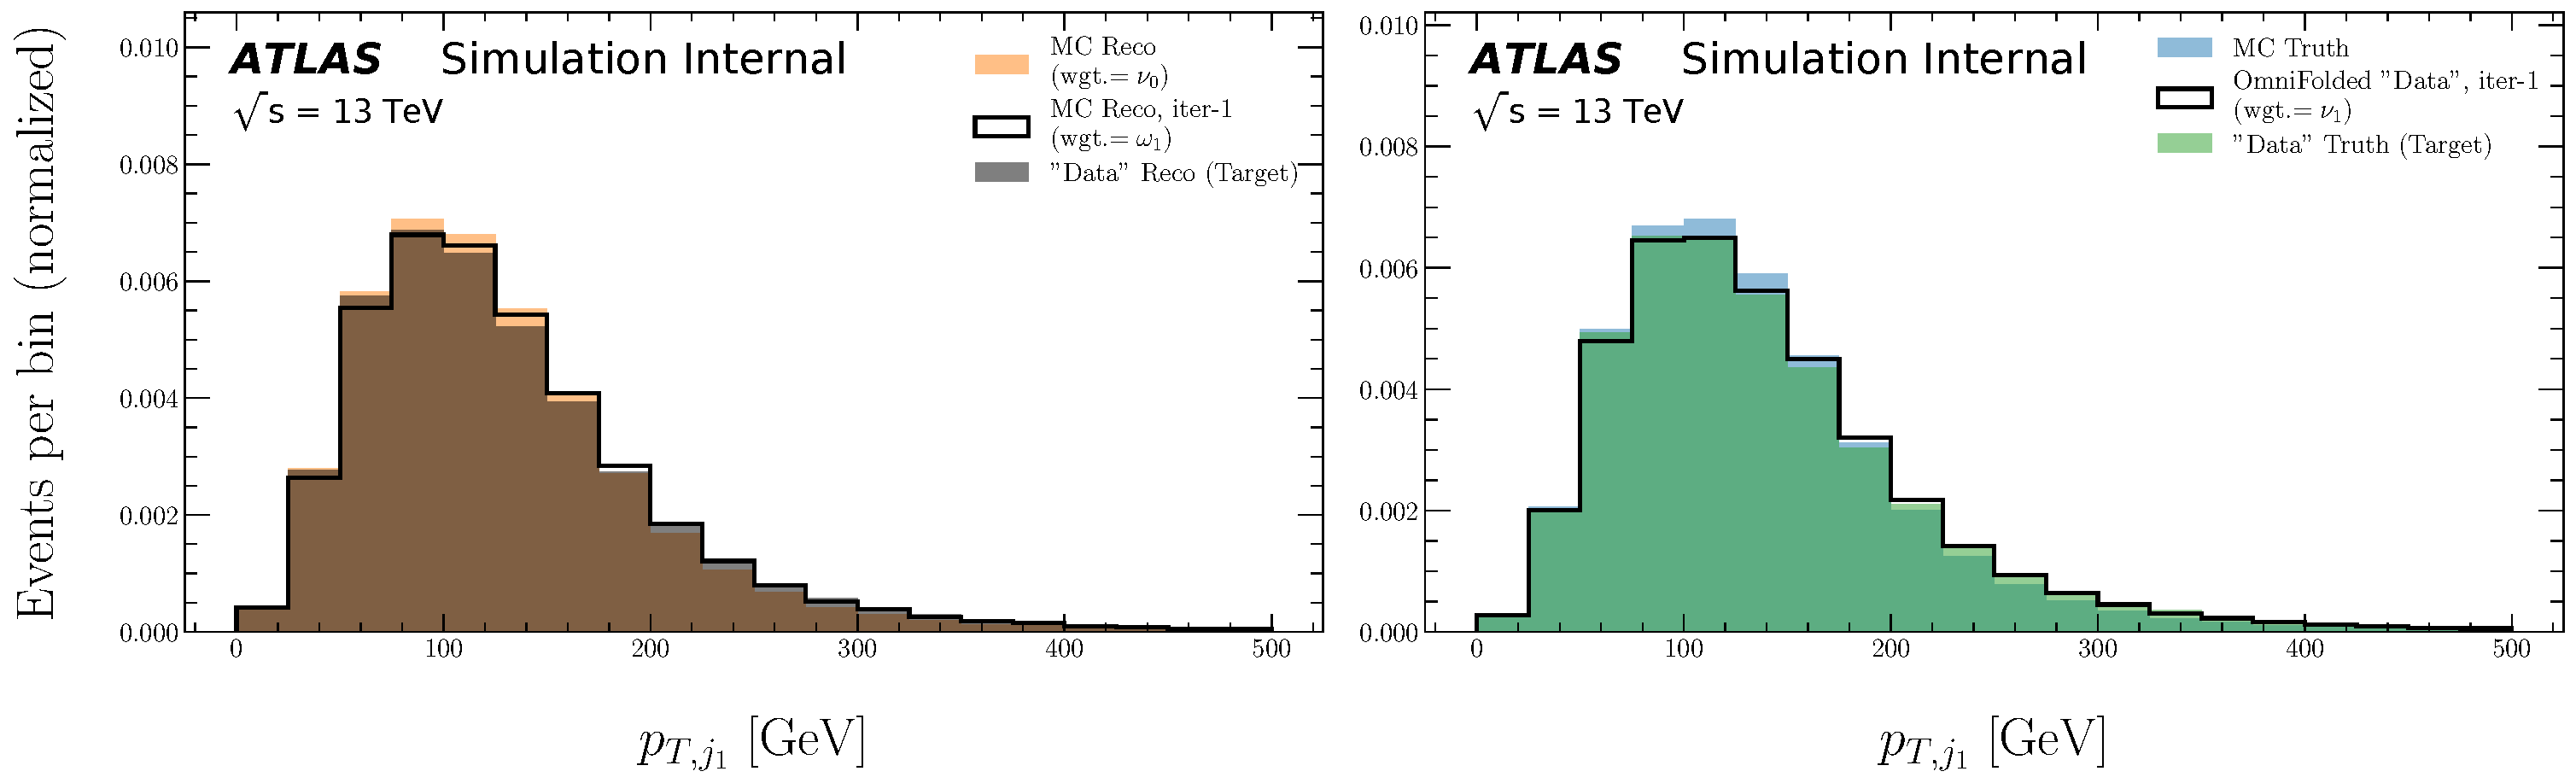
\includegraphics[width=0.85\textwidth]{figures/ATLASOmniFold-StressTest/ATLASOmniFold-StressTestC/UniFold/pT_trackj1/ATLASOmniFold-StressTestC-UniFold-pT_trackj1-Iteration01}}\\
\subfloat[After 2 iterations]{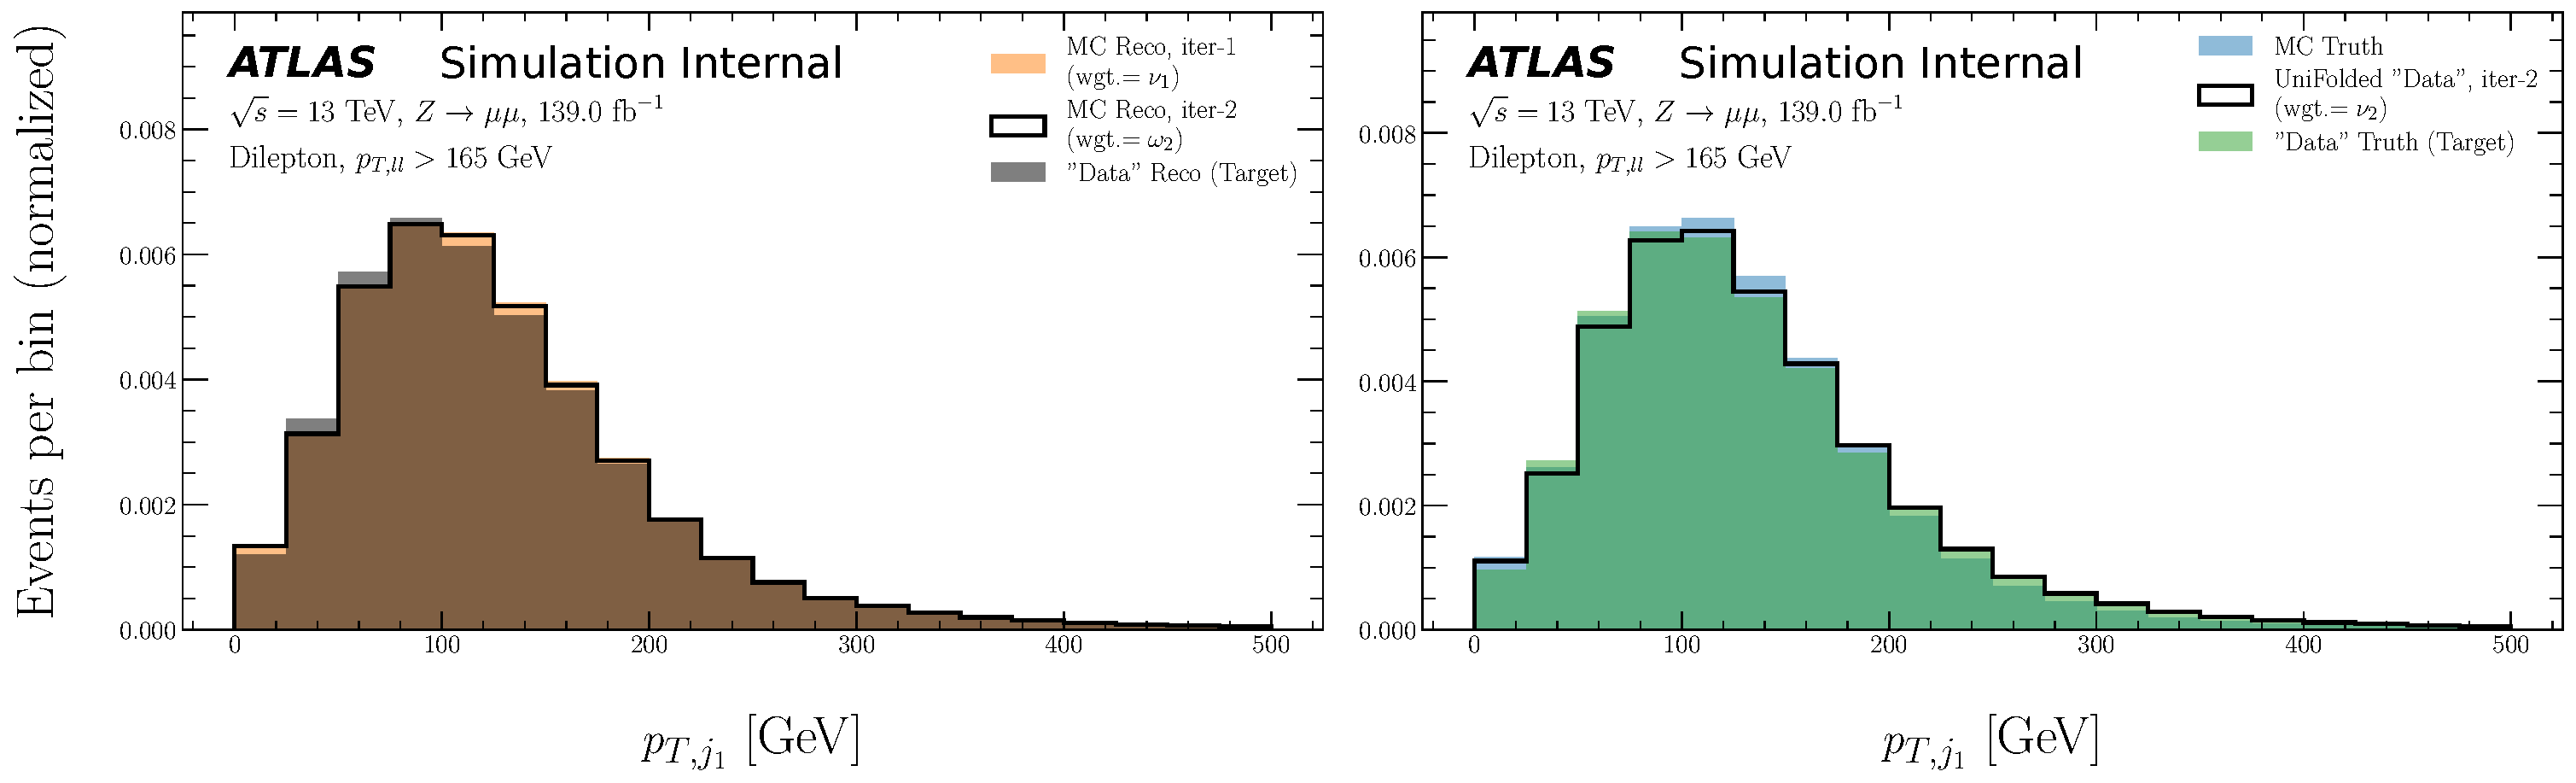
\includegraphics[width=0.85\textwidth]{figures/ATLASOmniFold-StressTest/ATLASOmniFold-StressTestC/UniFold/pT_trackj1/ATLASOmniFold-StressTestC-UniFold-pT_trackj1-Iteration02}}
\phantomcaption 
\end{figure}

\begin{figure}[h!]
\centering
\ContinuedFloat
\subfloat[After 3 iterations]{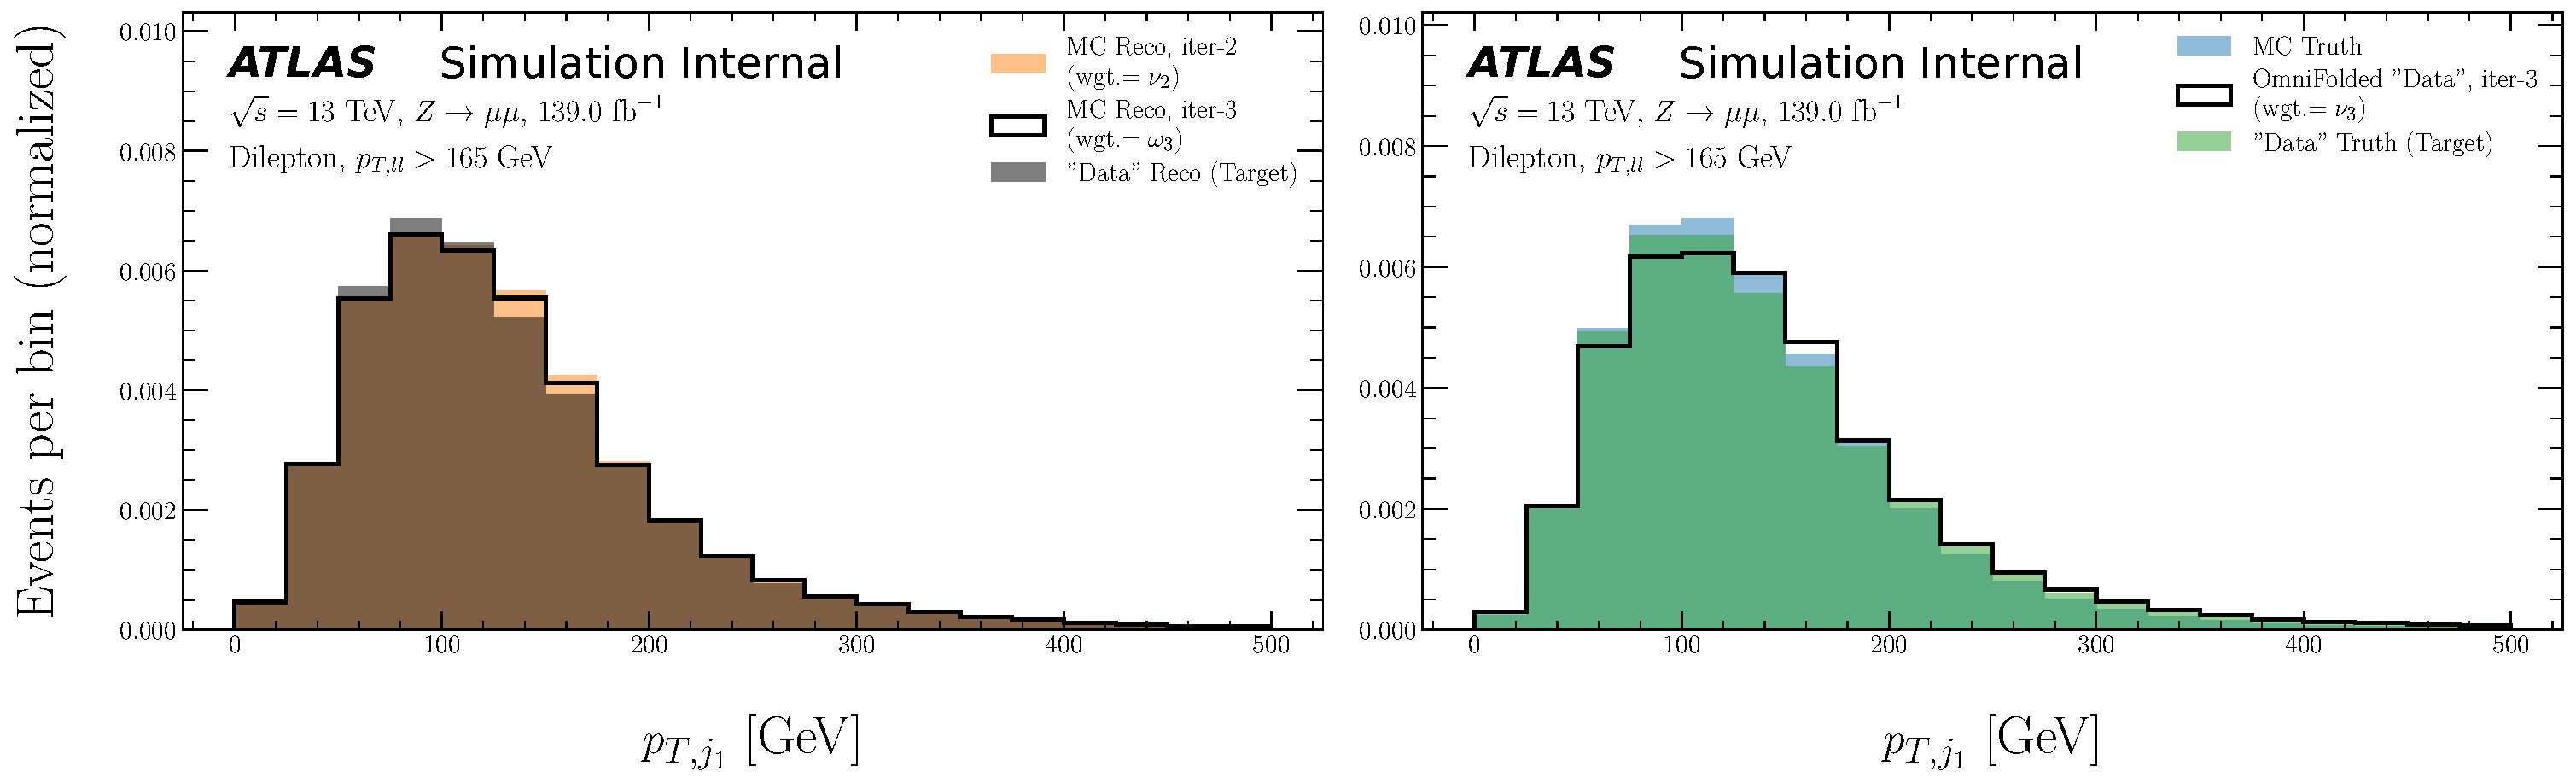
\includegraphics[width=0.85\textwidth]{figures/ATLASOmniFold-StressTest/ATLASOmniFold-StressTestC/UniFold/pT_trackj1/ATLASOmniFold-StressTestC-UniFold-pT_trackj1-Iteration03}}\\
\subfloat[After 4 iterations]{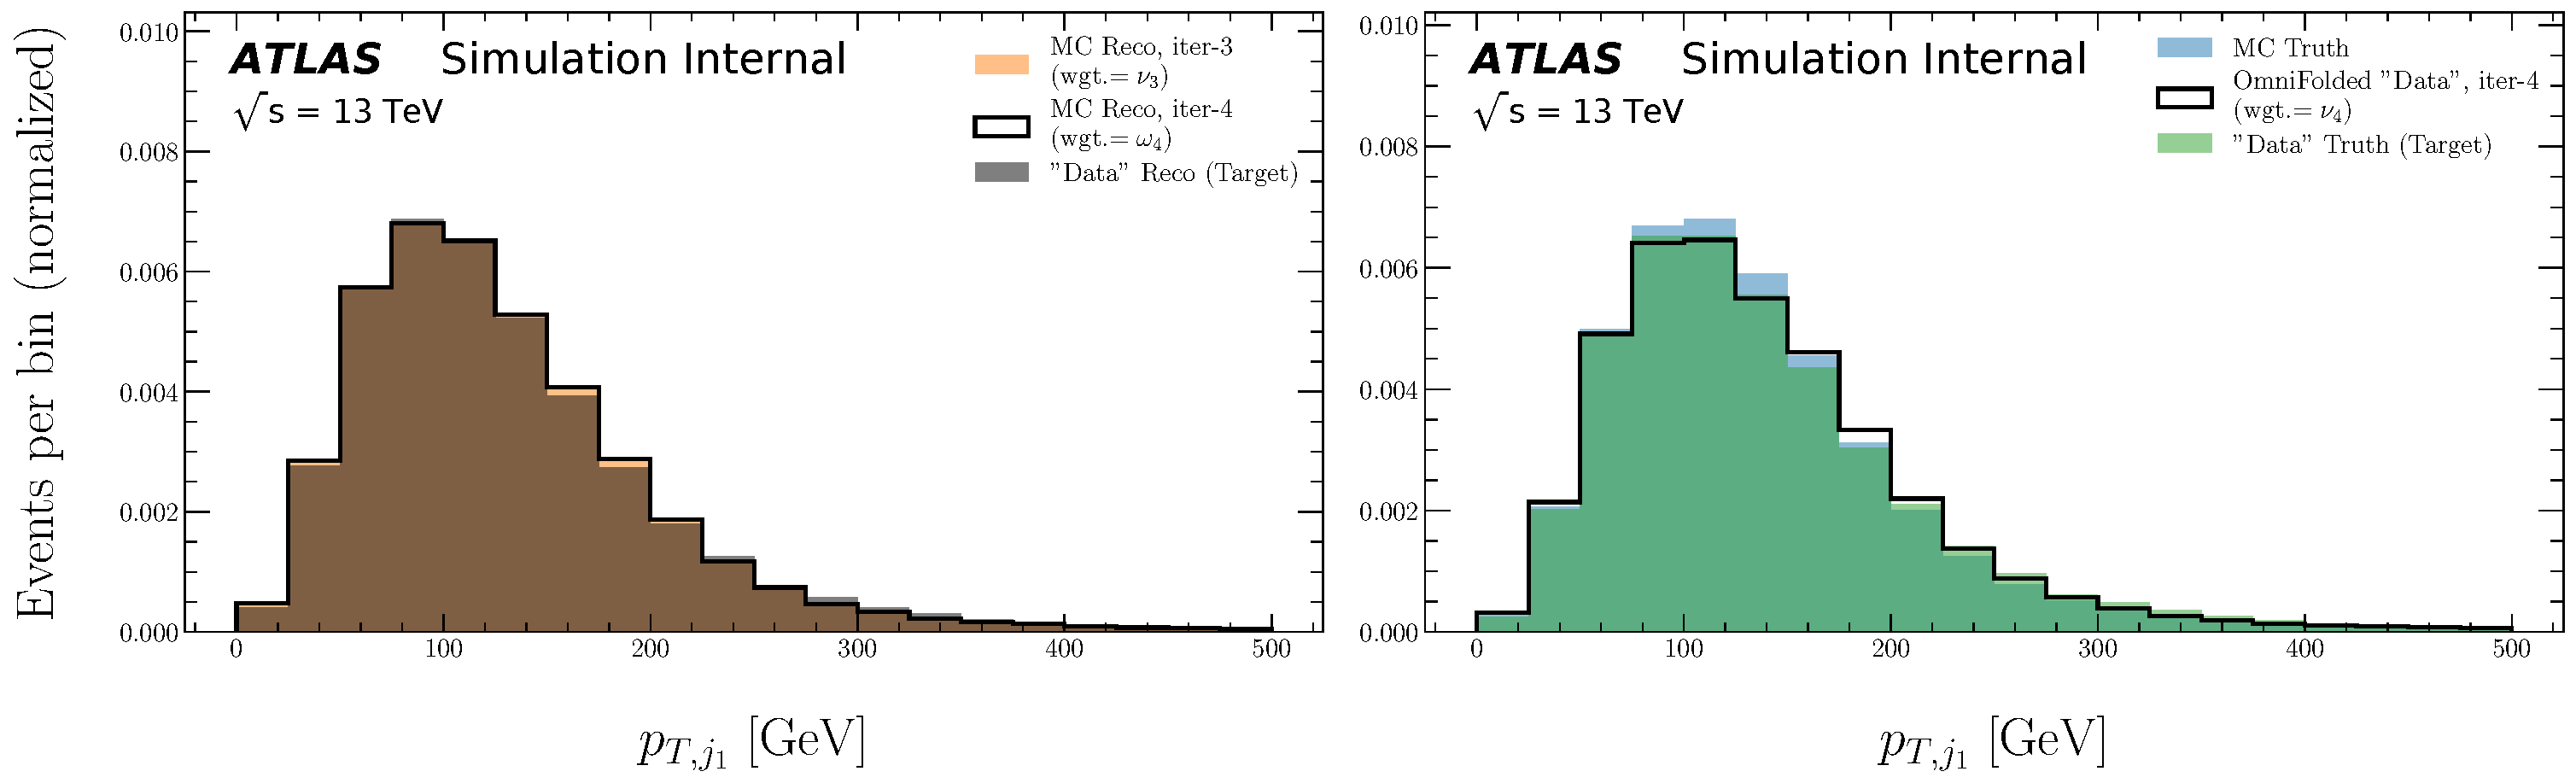
\includegraphics[width=0.85\textwidth]{figures/ATLASOmniFold-StressTest/ATLASOmniFold-StressTestC/UniFold/pT_trackj1/ATLASOmniFold-StressTestC-UniFold-pT_trackj1-Iteration04}}\\
\subfloat[After 5 iterations]{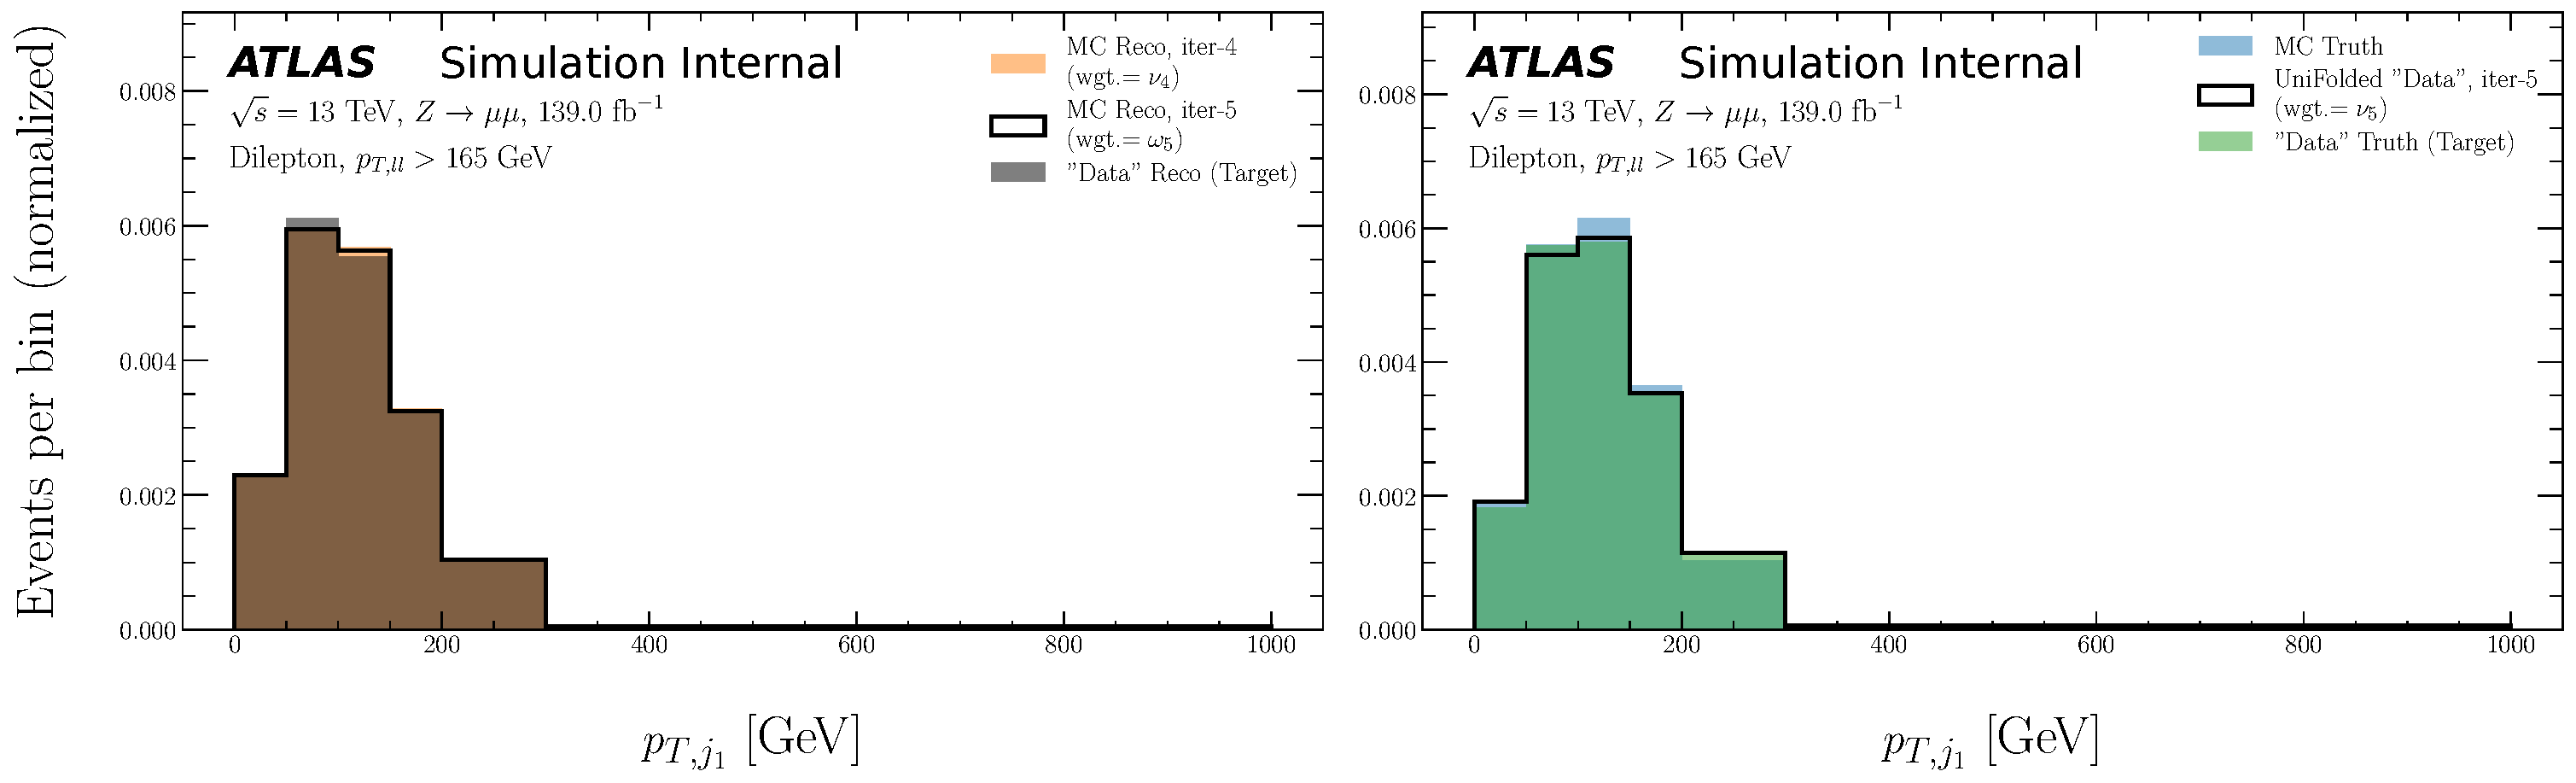
\includegraphics[width=0.85\textwidth]{figures/ATLASOmniFold-StressTest/ATLASOmniFold-StressTestC/UniFold/pT_trackj1/ATLASOmniFold-StressTestC-UniFold-pT_trackj1-Iteration05}}\\
\subfloat[After 6 iterations]{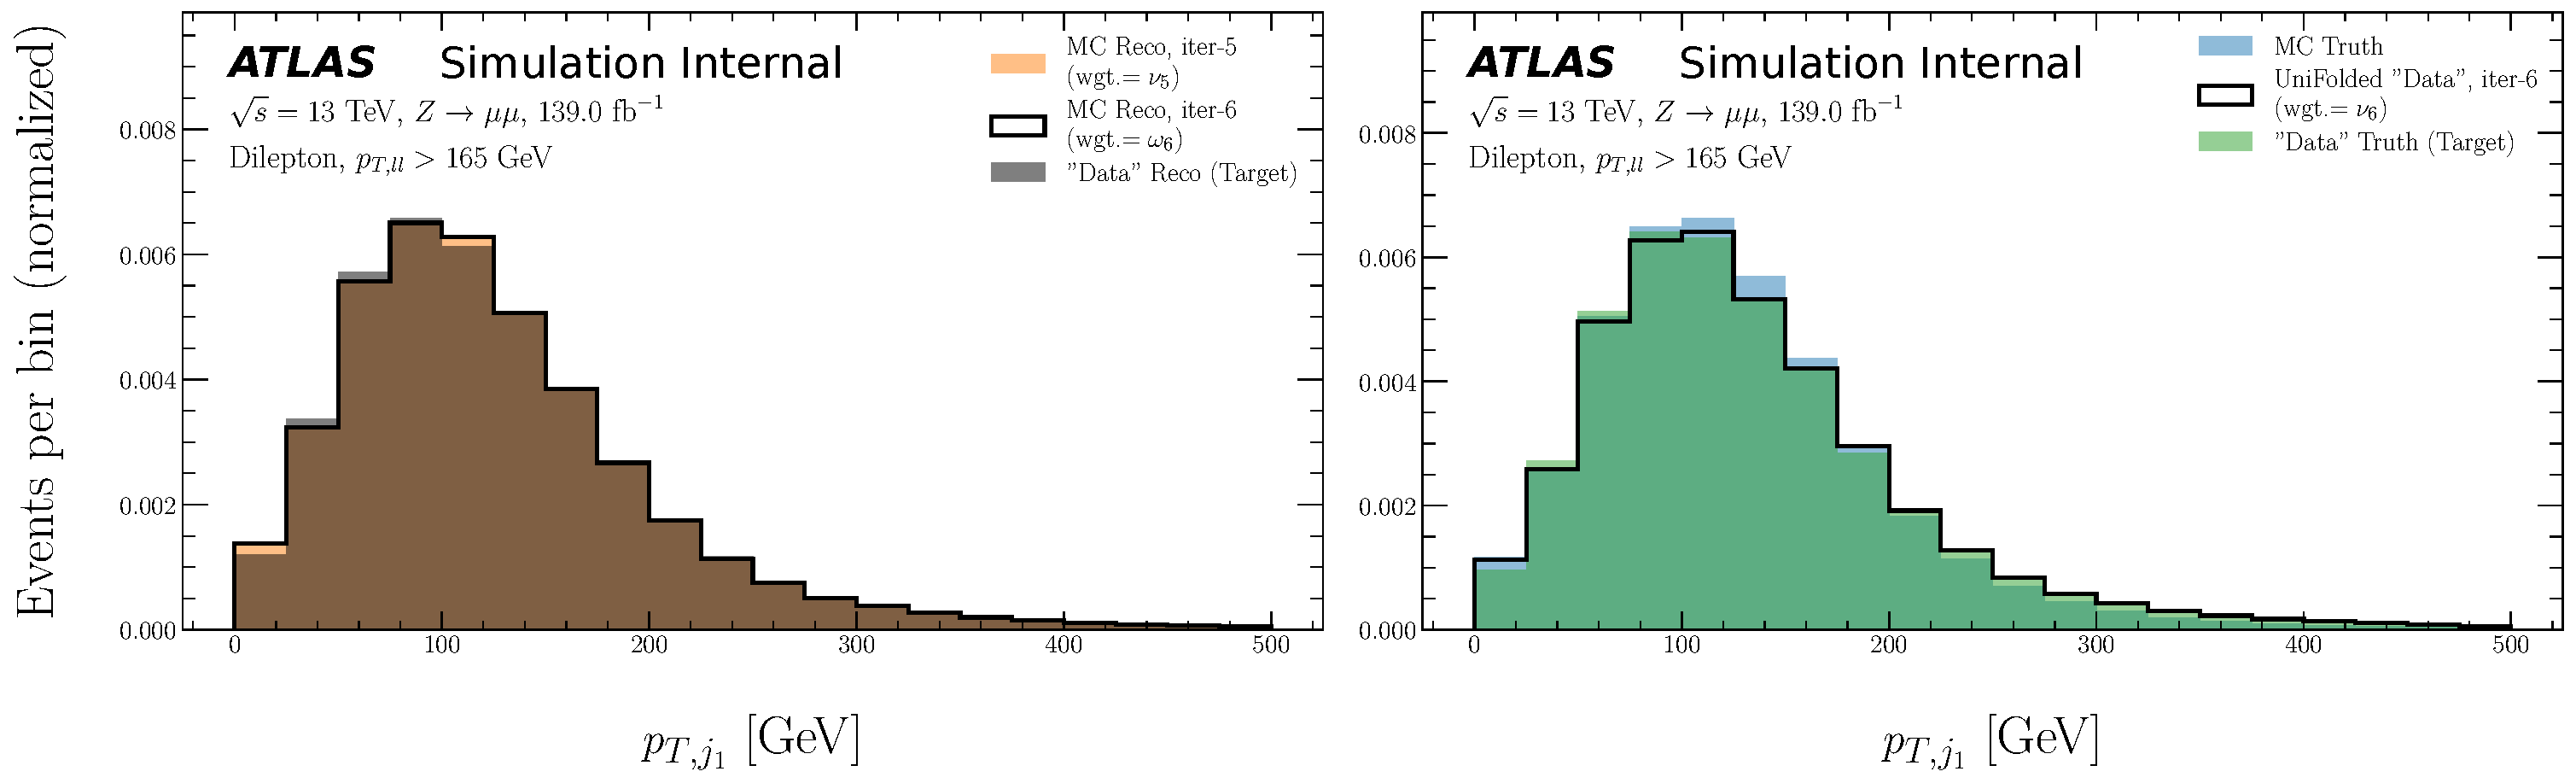
\includegraphics[width=0.85\textwidth]{figures/ATLASOmniFold-StressTest/ATLASOmniFold-StressTestC/UniFold/pT_trackj1/ATLASOmniFold-StressTestC-UniFold-pT_trackj1-Iteration06}}
\caption{UniFolding Sherpa with Pythia for the leading track jet $p_T$.}
\label{fig:stressc_pT_trackj1}
\end{figure}

\begin{figure}[h!]
\centering
\subfloat[Input histograms]{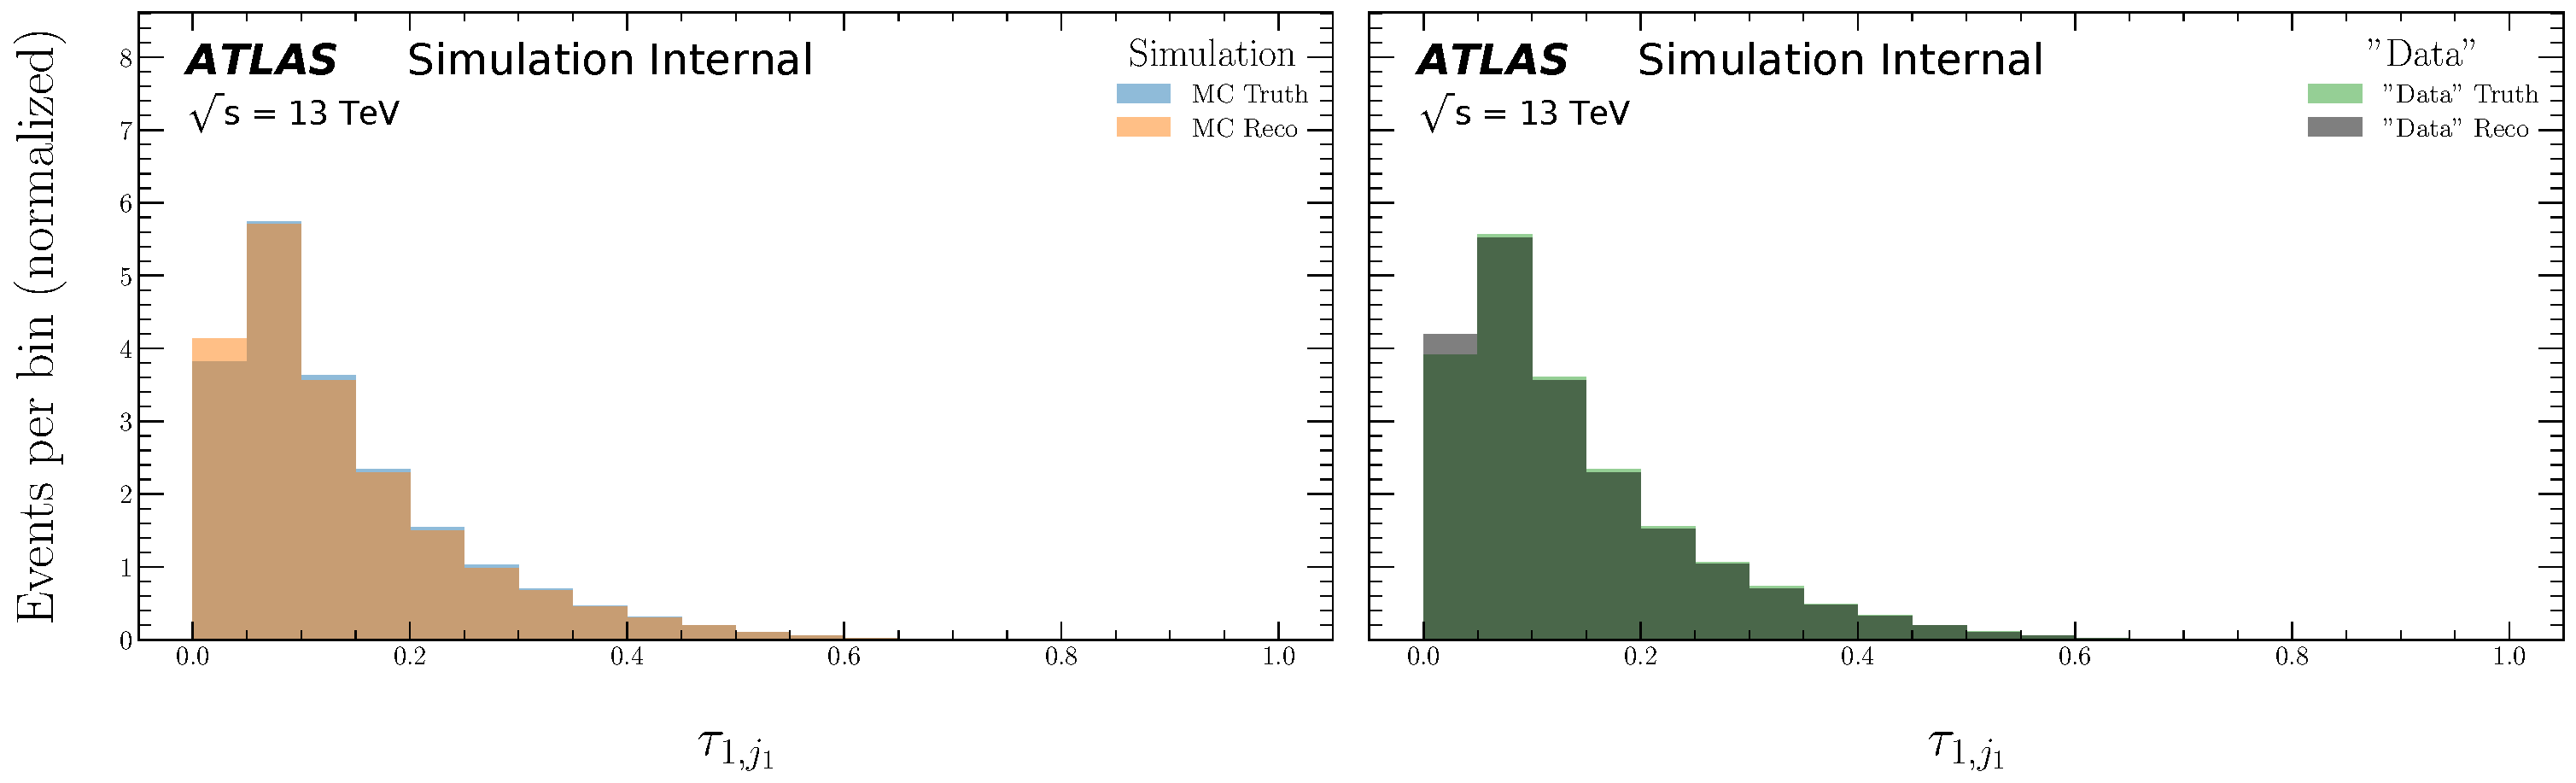
\includegraphics[width=0.85\textwidth]{figures/ATLASOmniFold-StressTest/ATLASOmniFold-StressTestC/UniFold/tau1_trackj1/ATLASOmniFold-StressTestC-UniFold-tau1_trackj1-Distributions}}\\
\subfloat[After 1 iteration]{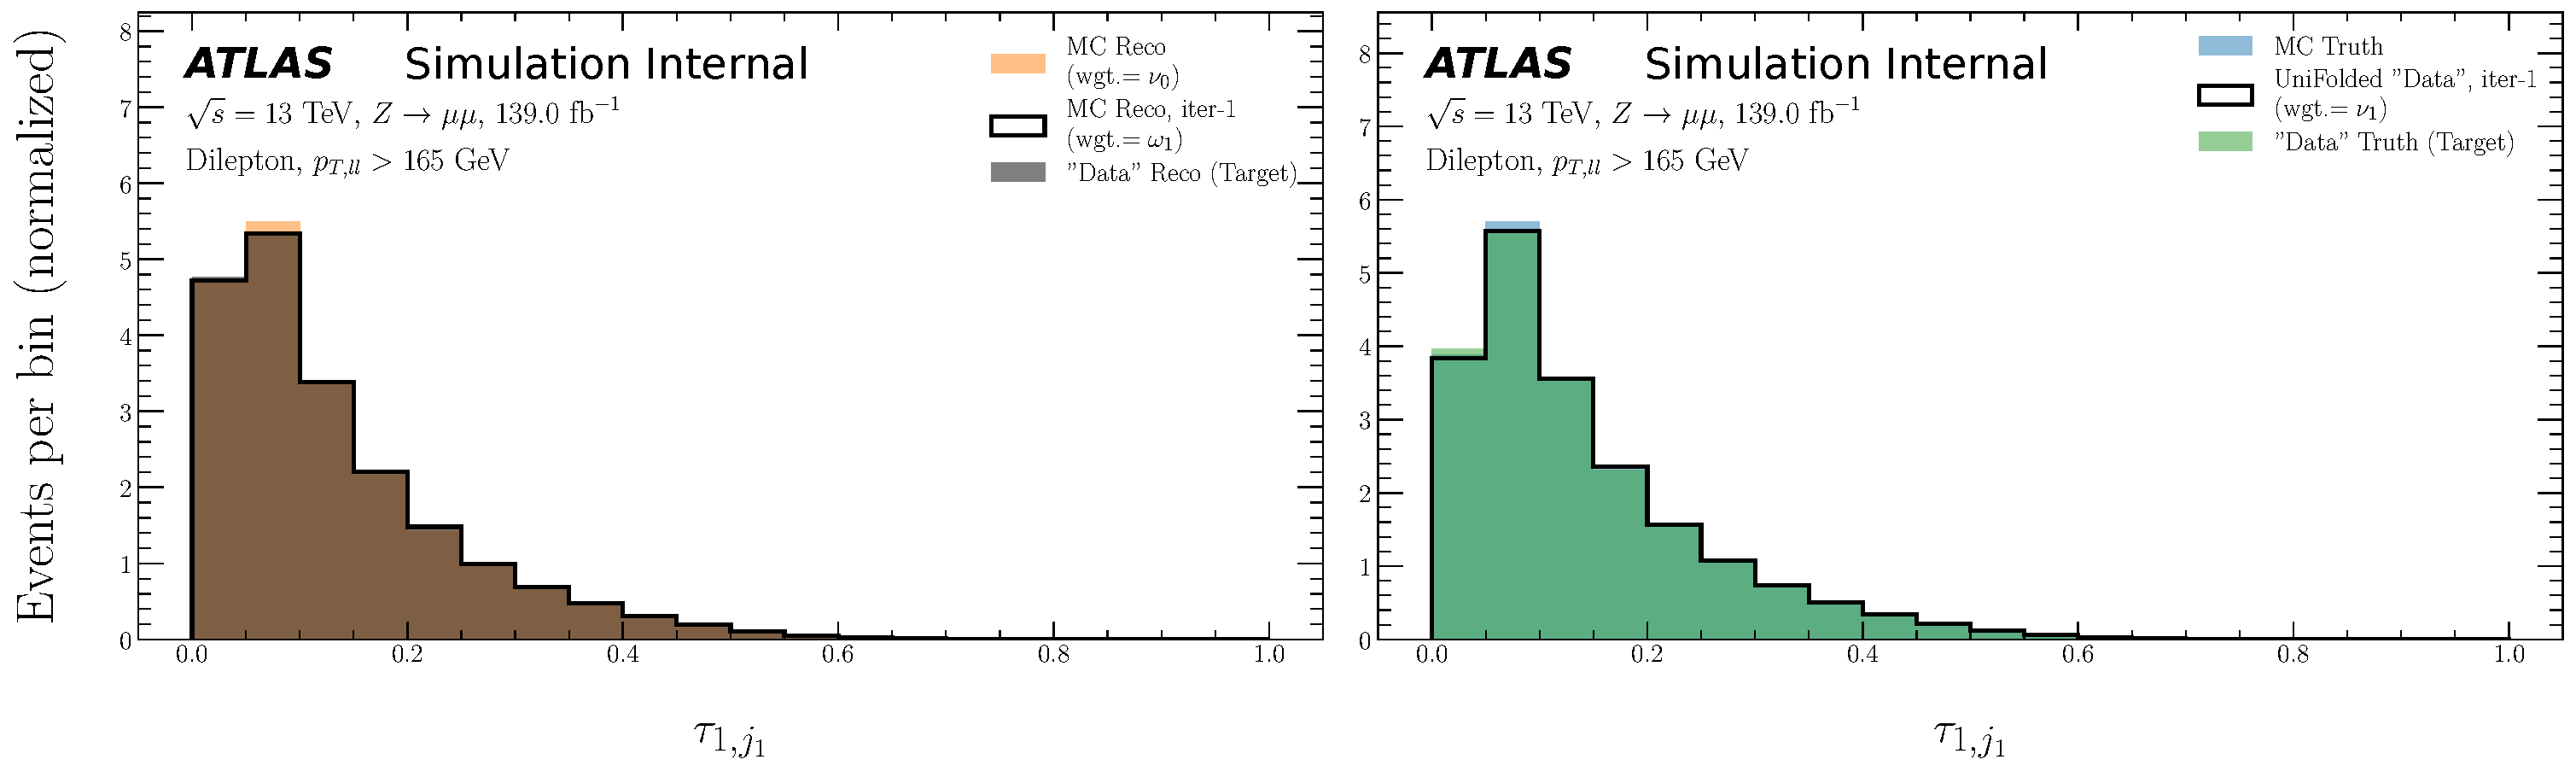
\includegraphics[width=0.85\textwidth]{figures/ATLASOmniFold-StressTest/ATLASOmniFold-StressTestC/UniFold/tau1_trackj1/ATLASOmniFold-StressTestC-UniFold-tau1_trackj1-Iteration01}}\\
\subfloat[After 2 iterations]{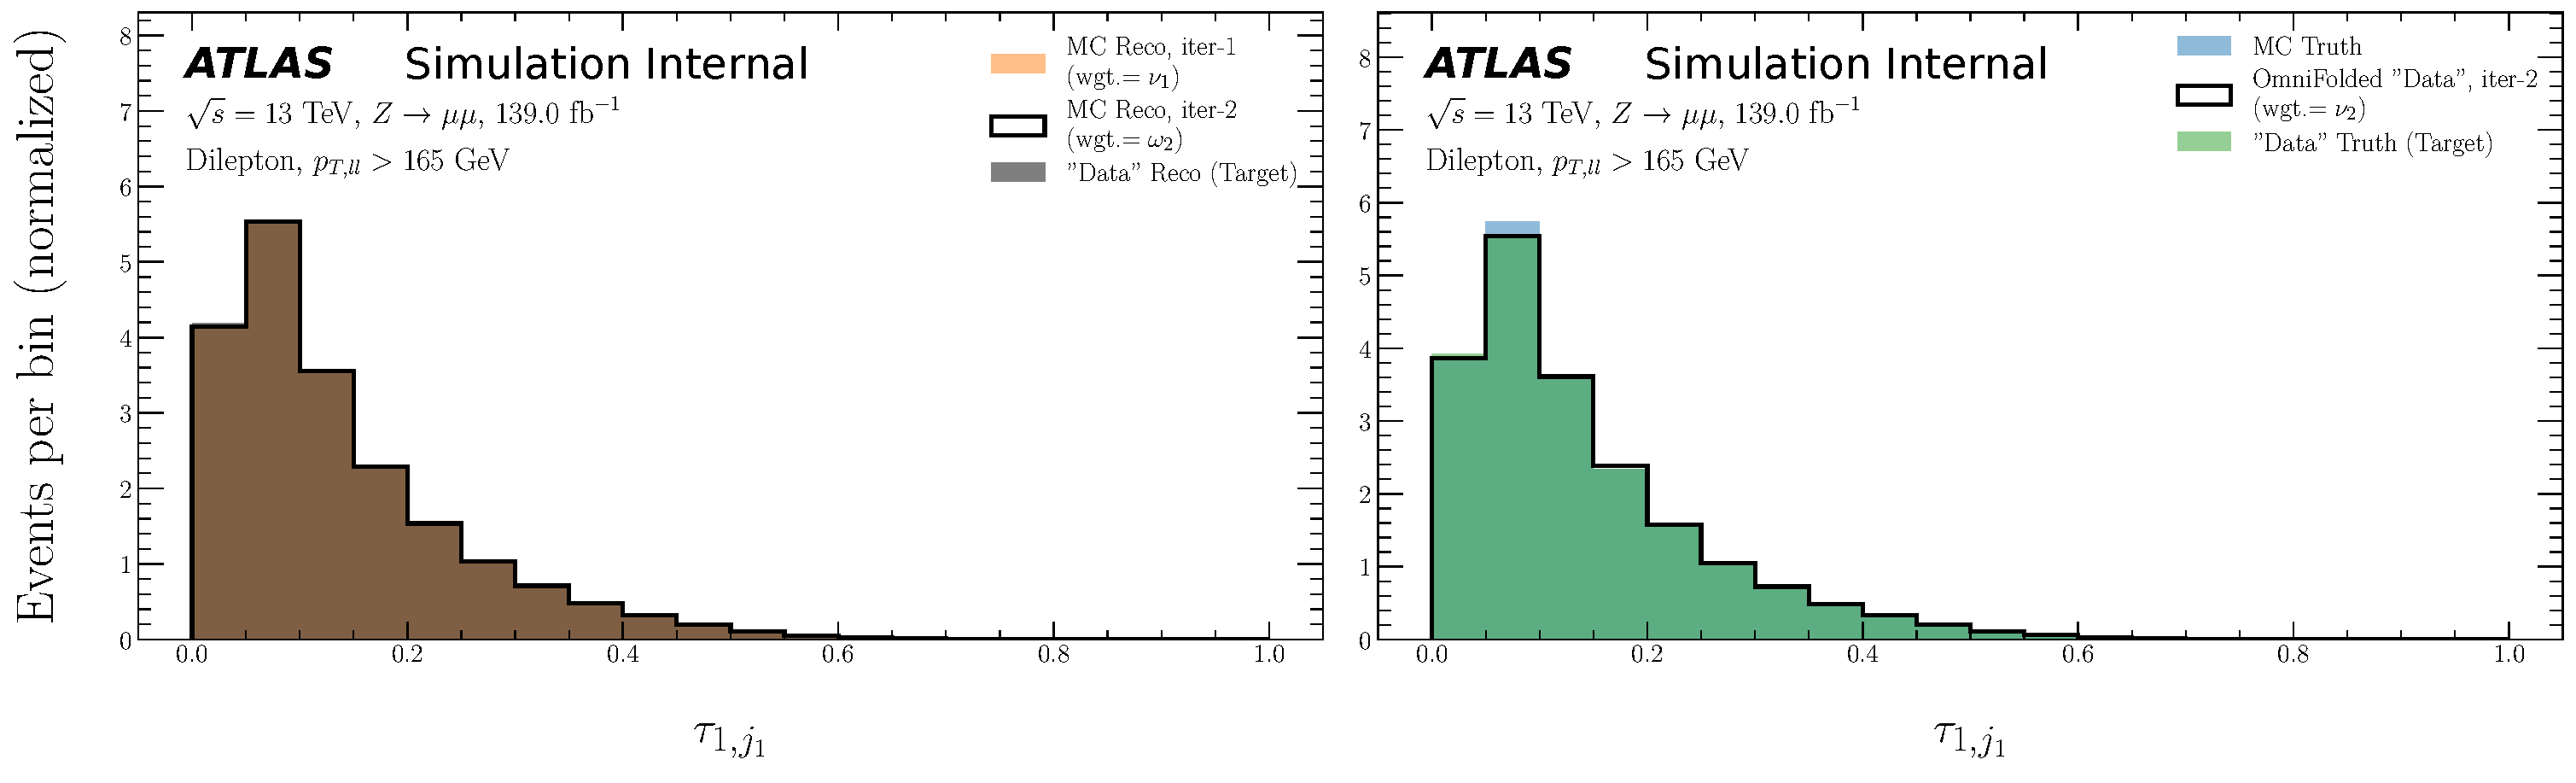
\includegraphics[width=0.85\textwidth]{figures/ATLASOmniFold-StressTest/ATLASOmniFold-StressTestC/UniFold/tau1_trackj1/ATLASOmniFold-StressTestC-UniFold-tau1_trackj1-Iteration02}}
\phantomcaption 
\end{figure}

\begin{figure}[h!]
\centering
\ContinuedFloat
\subfloat[After 3 iterations]{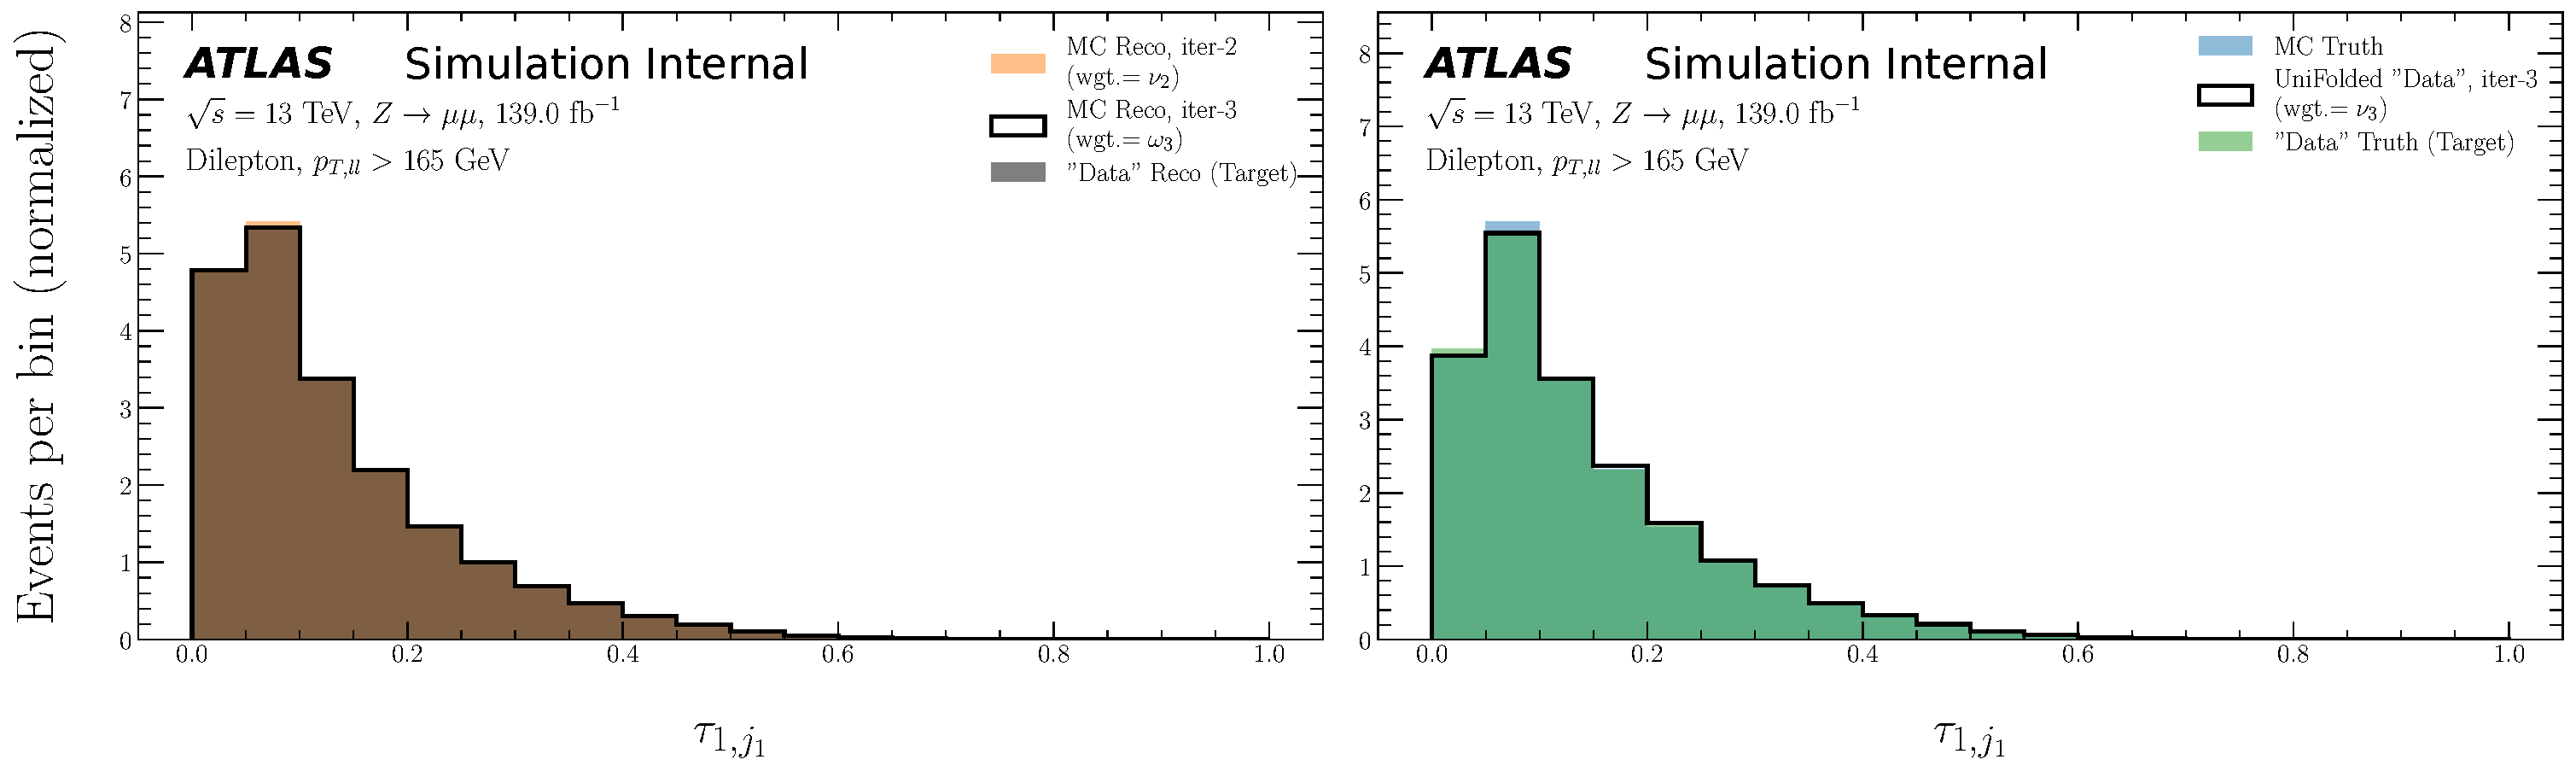
\includegraphics[width=0.85\textwidth]{figures/ATLASOmniFold-StressTest/ATLASOmniFold-StressTestC/UniFold/tau1_trackj1/ATLASOmniFold-StressTestC-UniFold-tau1_trackj1-Iteration03}}\\
\subfloat[After 4 iterations]{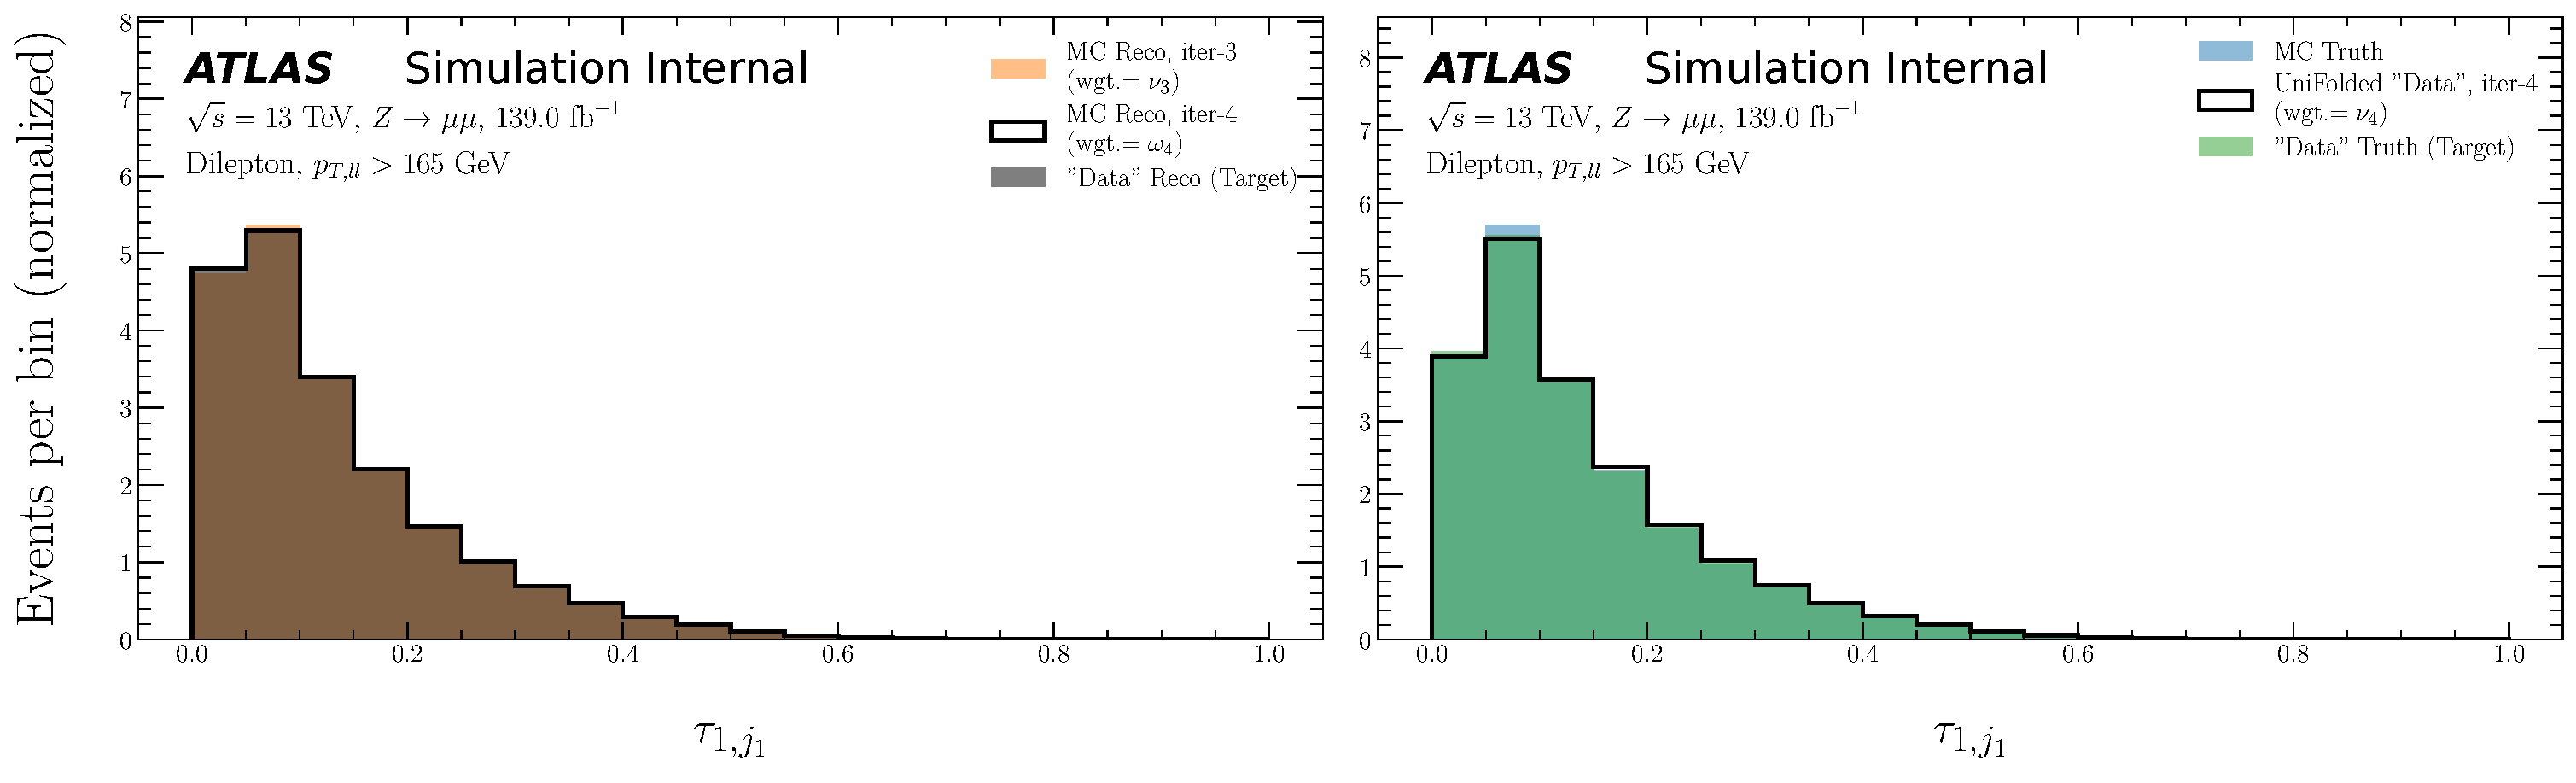
\includegraphics[width=0.85\textwidth]{figures/ATLASOmniFold-StressTest/ATLASOmniFold-StressTestC/UniFold/tau1_trackj1/ATLASOmniFold-StressTestC-UniFold-tau1_trackj1-Iteration04}}\\
\subfloat[After 5 iterations]{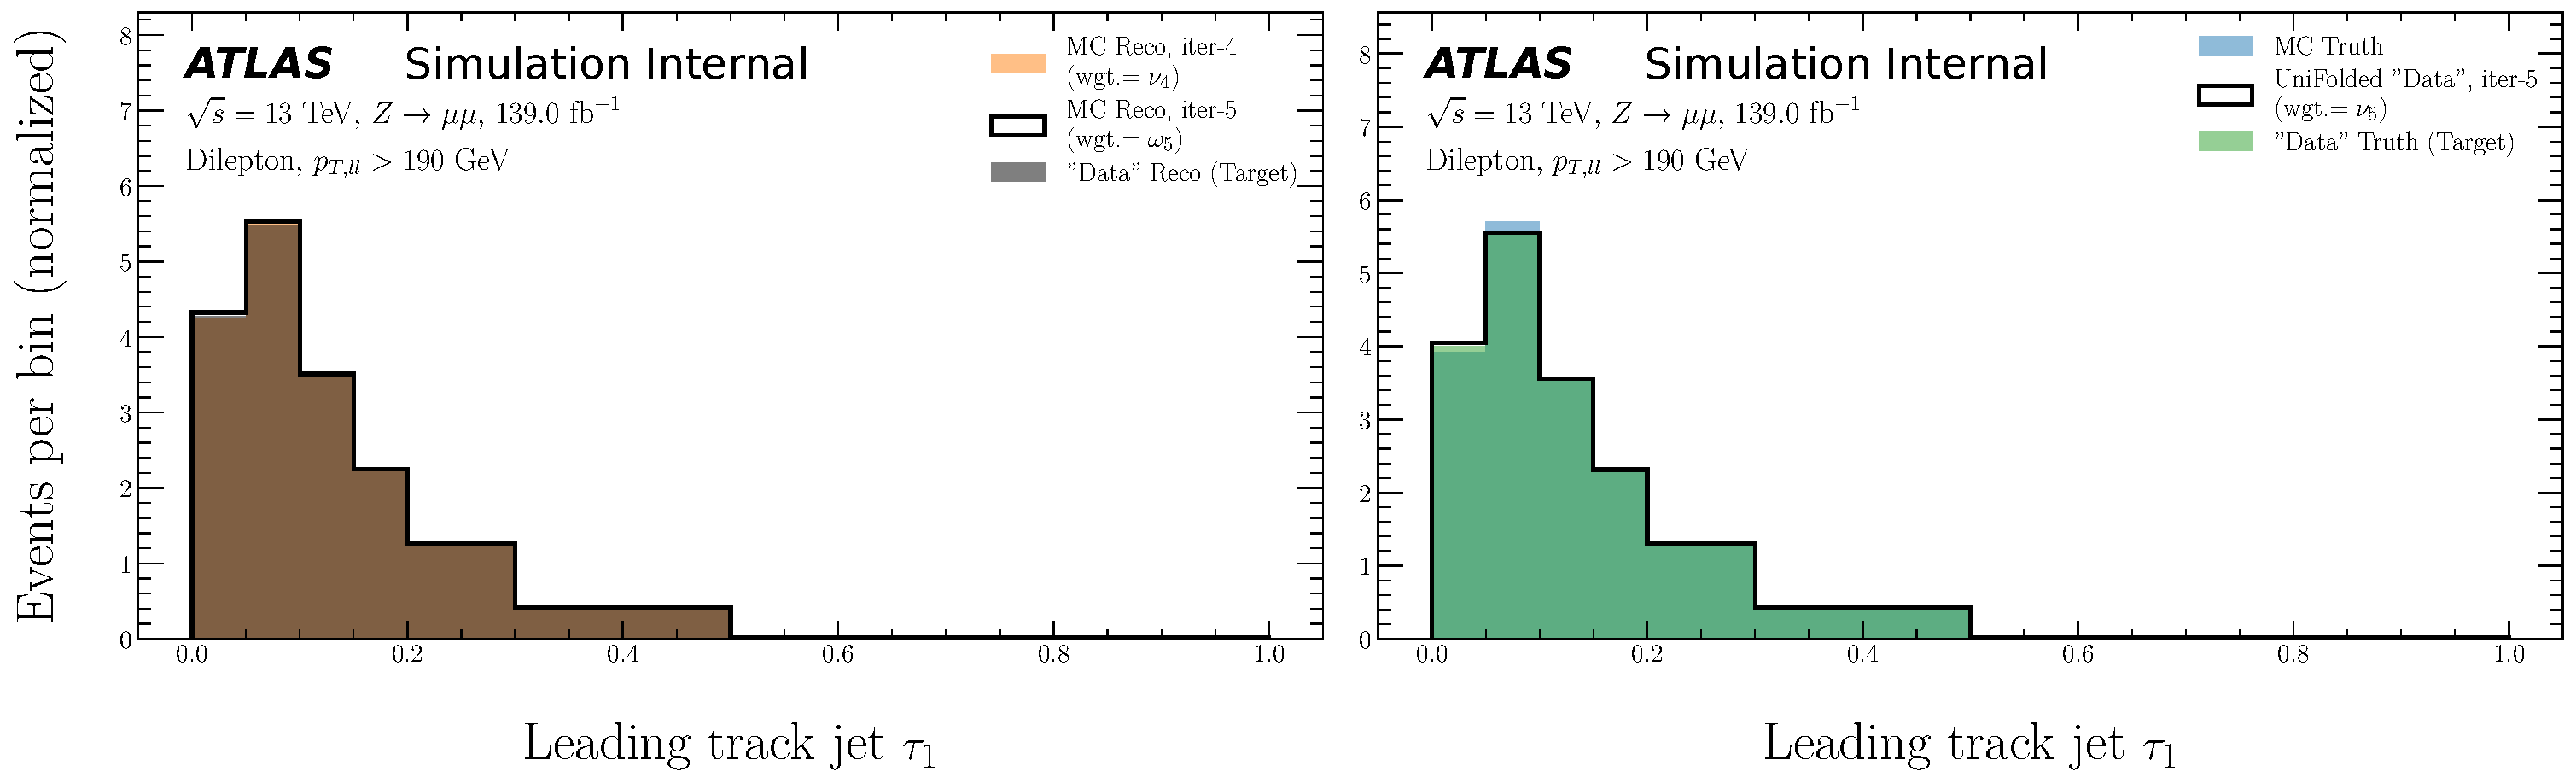
\includegraphics[width=0.85\textwidth]{figures/ATLASOmniFold-StressTest/ATLASOmniFold-StressTestC/UniFold/tau1_trackj1/ATLASOmniFold-StressTestC-UniFold-tau1_trackj1-Iteration05}}\\
\subfloat[After 6 iterations]{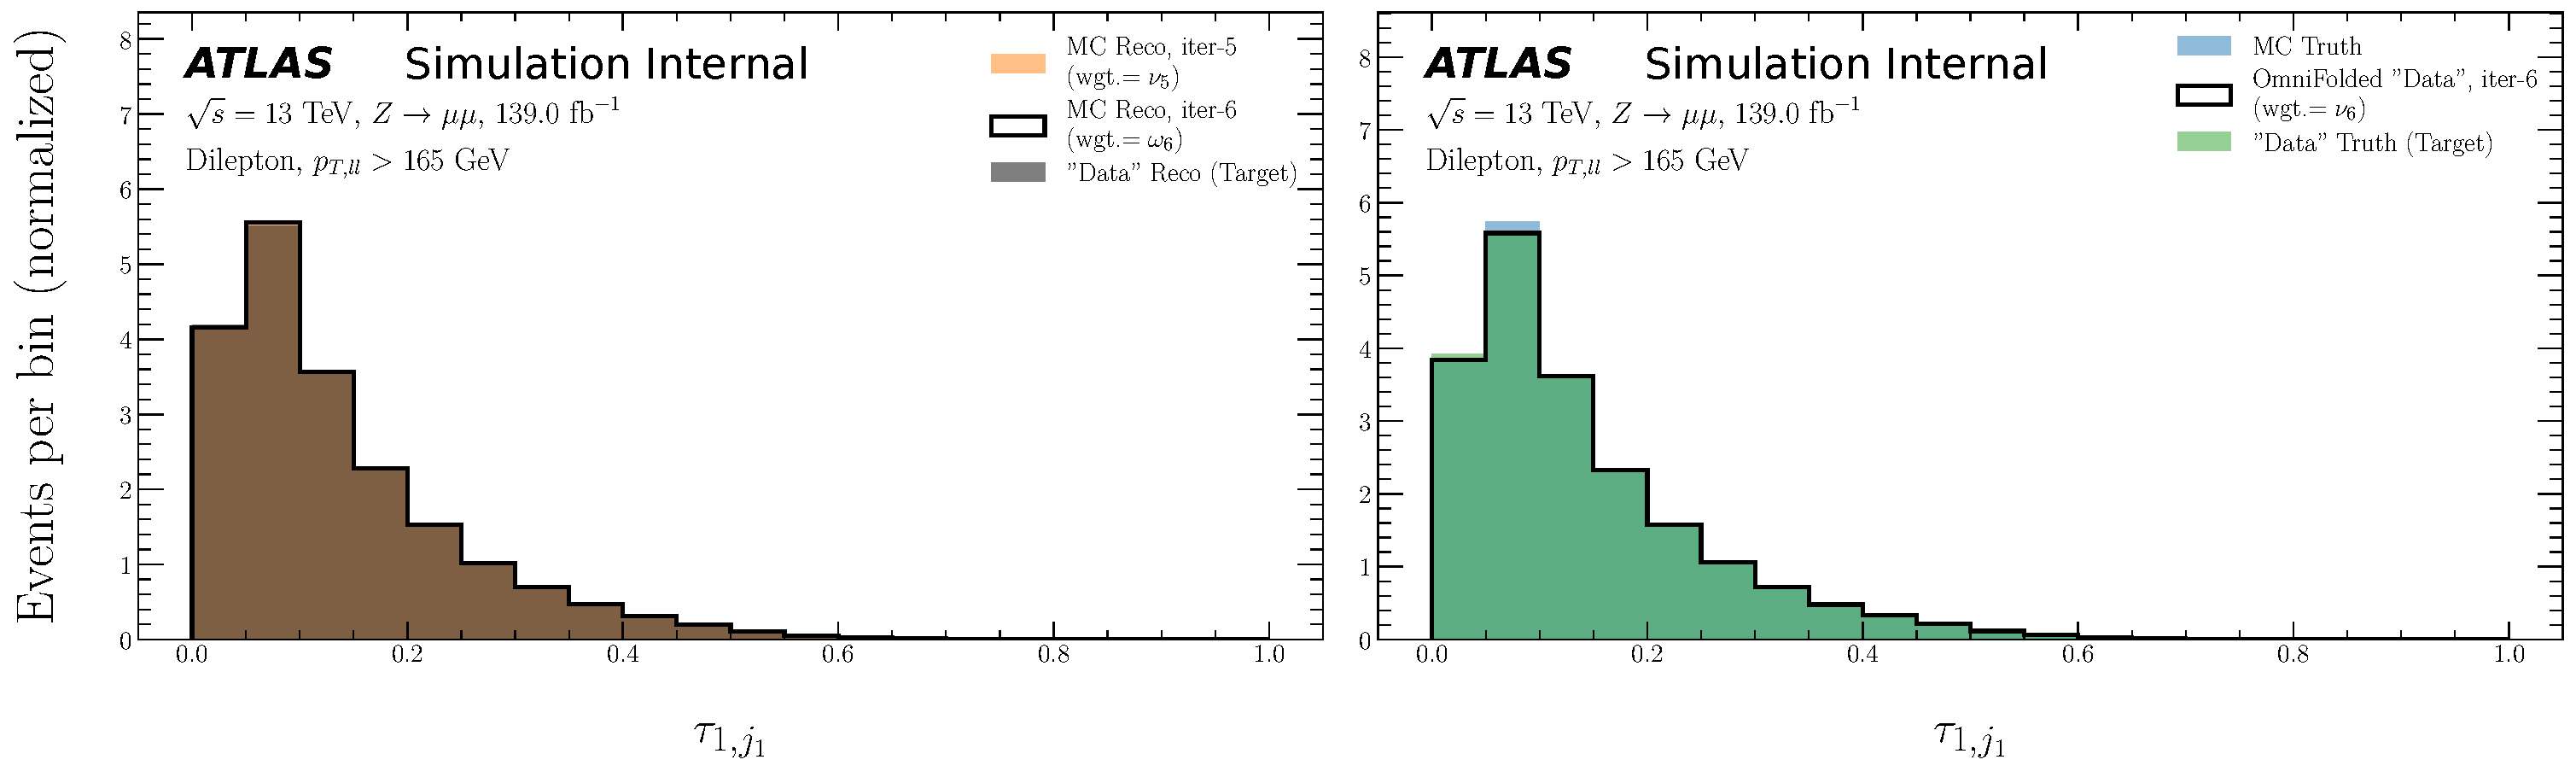
\includegraphics[width=0.85\textwidth]{figures/ATLASOmniFold-StressTest/ATLASOmniFold-StressTestC/UniFold/tau1_trackj1/ATLASOmniFold-StressTestC-UniFold-tau1_trackj1-Iteration06}}
\caption{UniFolding Sherpa with Pythia for the leading track jet $\tau_1$.}
\label{fig:stressc_tau1_trackj1}
\end{figure}

\begin{figure}[h!]
\centering
\subfloat[Input histograms]{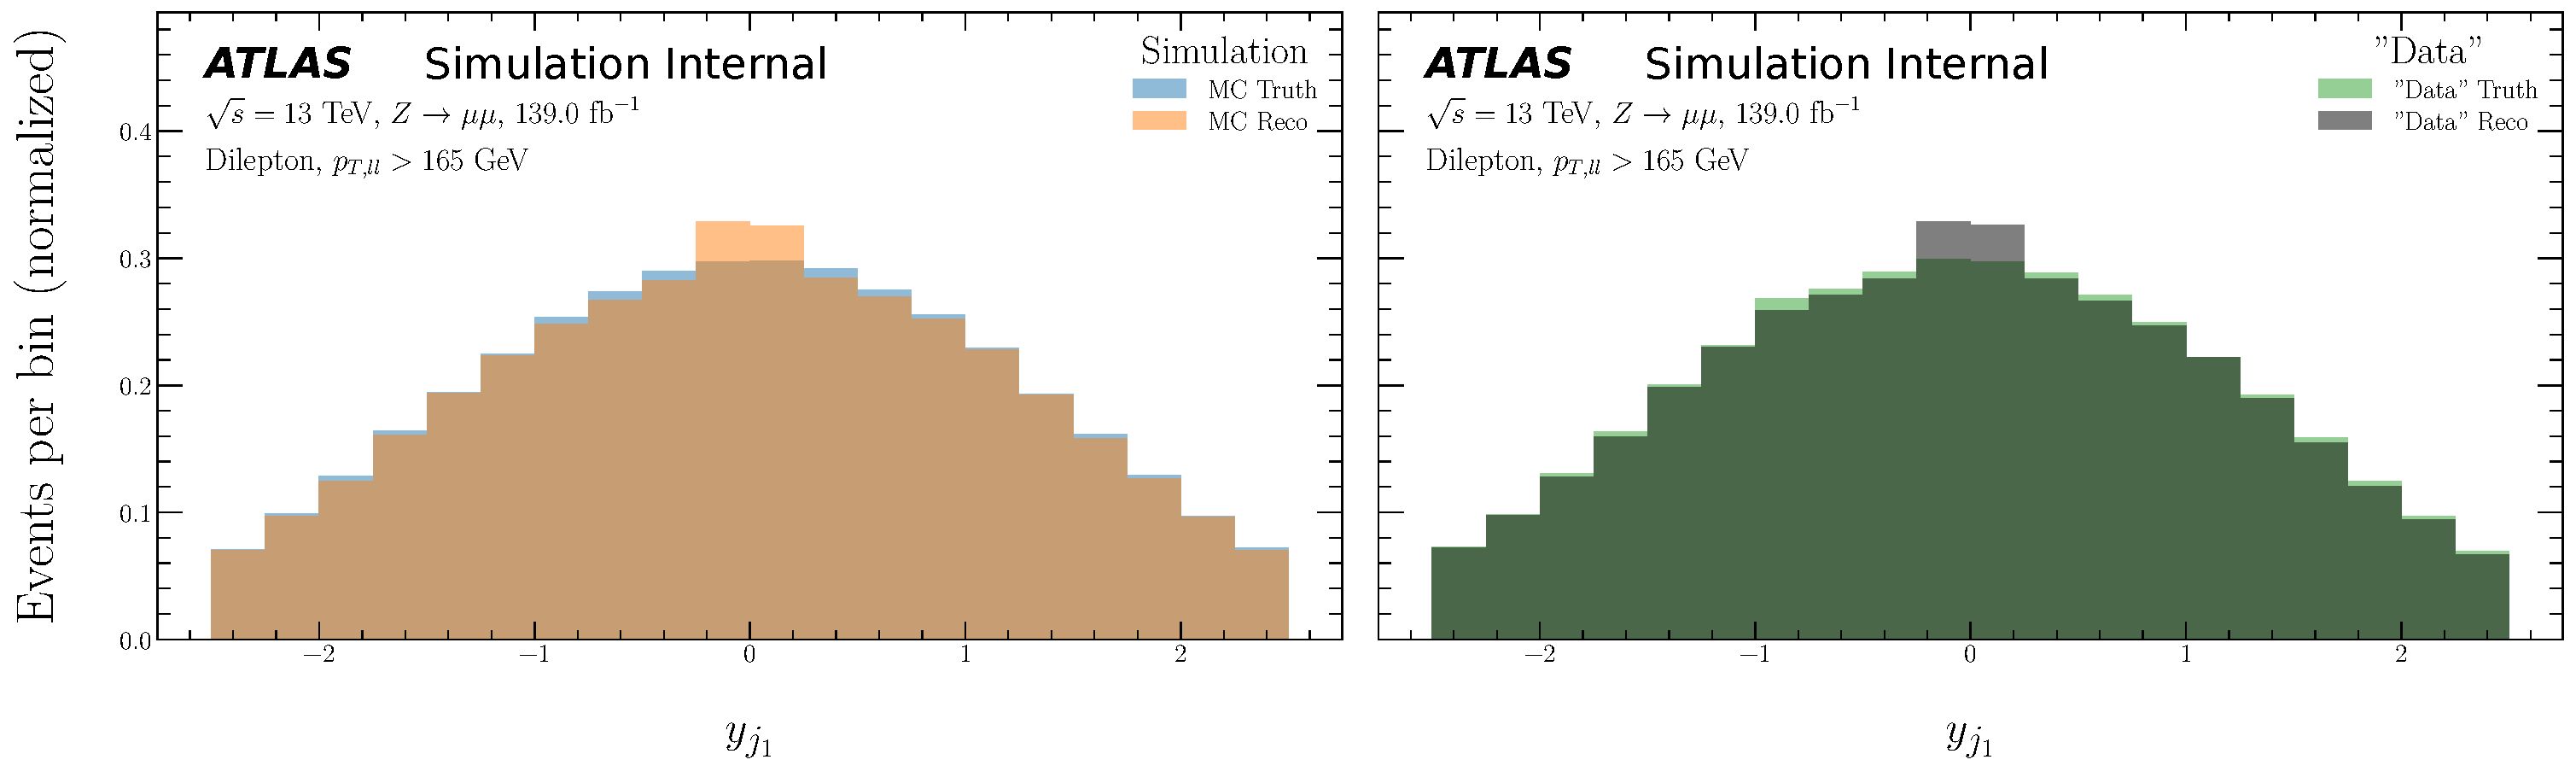
\includegraphics[width=0.85\textwidth]{figures/ATLASOmniFold-StressTest/ATLASOmniFold-StressTestC/UniFold/y_trackj1/ATLASOmniFold-StressTestC-UniFold-y_trackj1-Distributions}}\\
\subfloat[After 1 iteration]{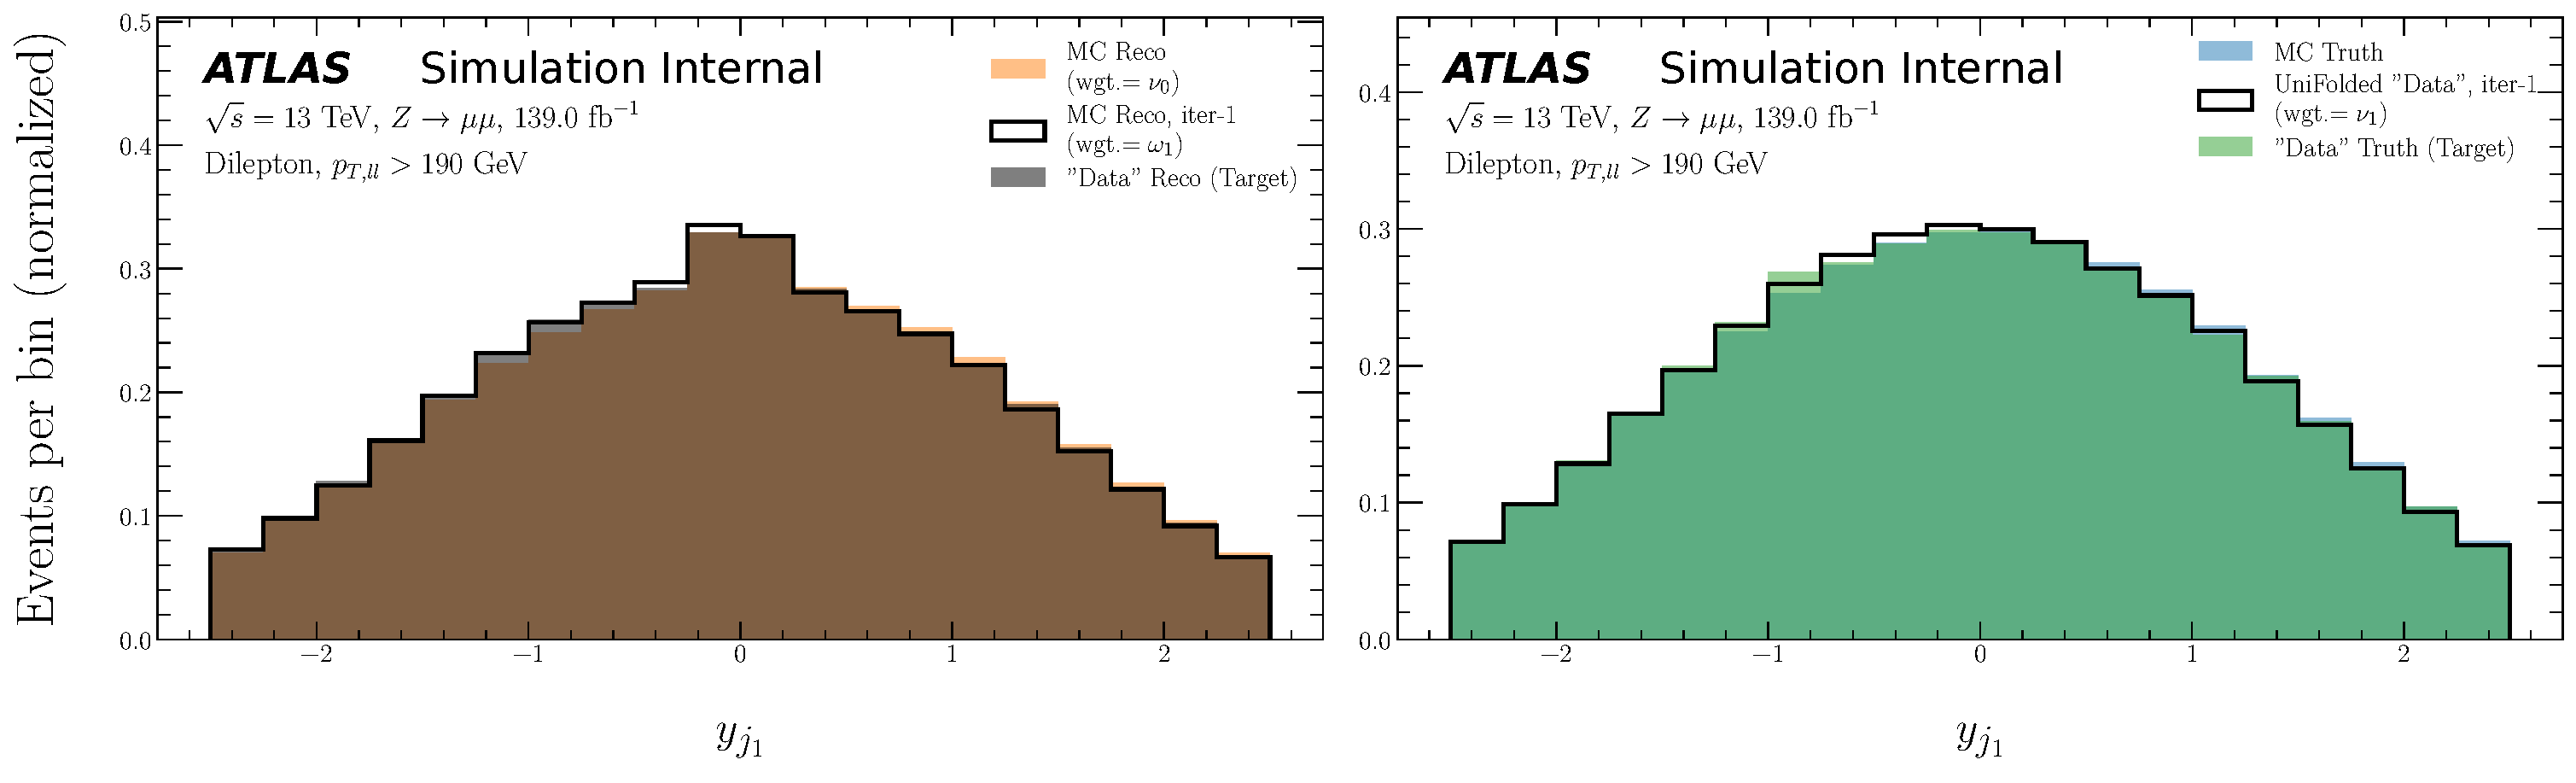
\includegraphics[width=0.85\textwidth]{figures/ATLASOmniFold-StressTest/ATLASOmniFold-StressTestC/UniFold/y_trackj1/ATLASOmniFold-StressTestC-UniFold-y_trackj1-Iteration01}}\\
\subfloat[After 2 iterations]{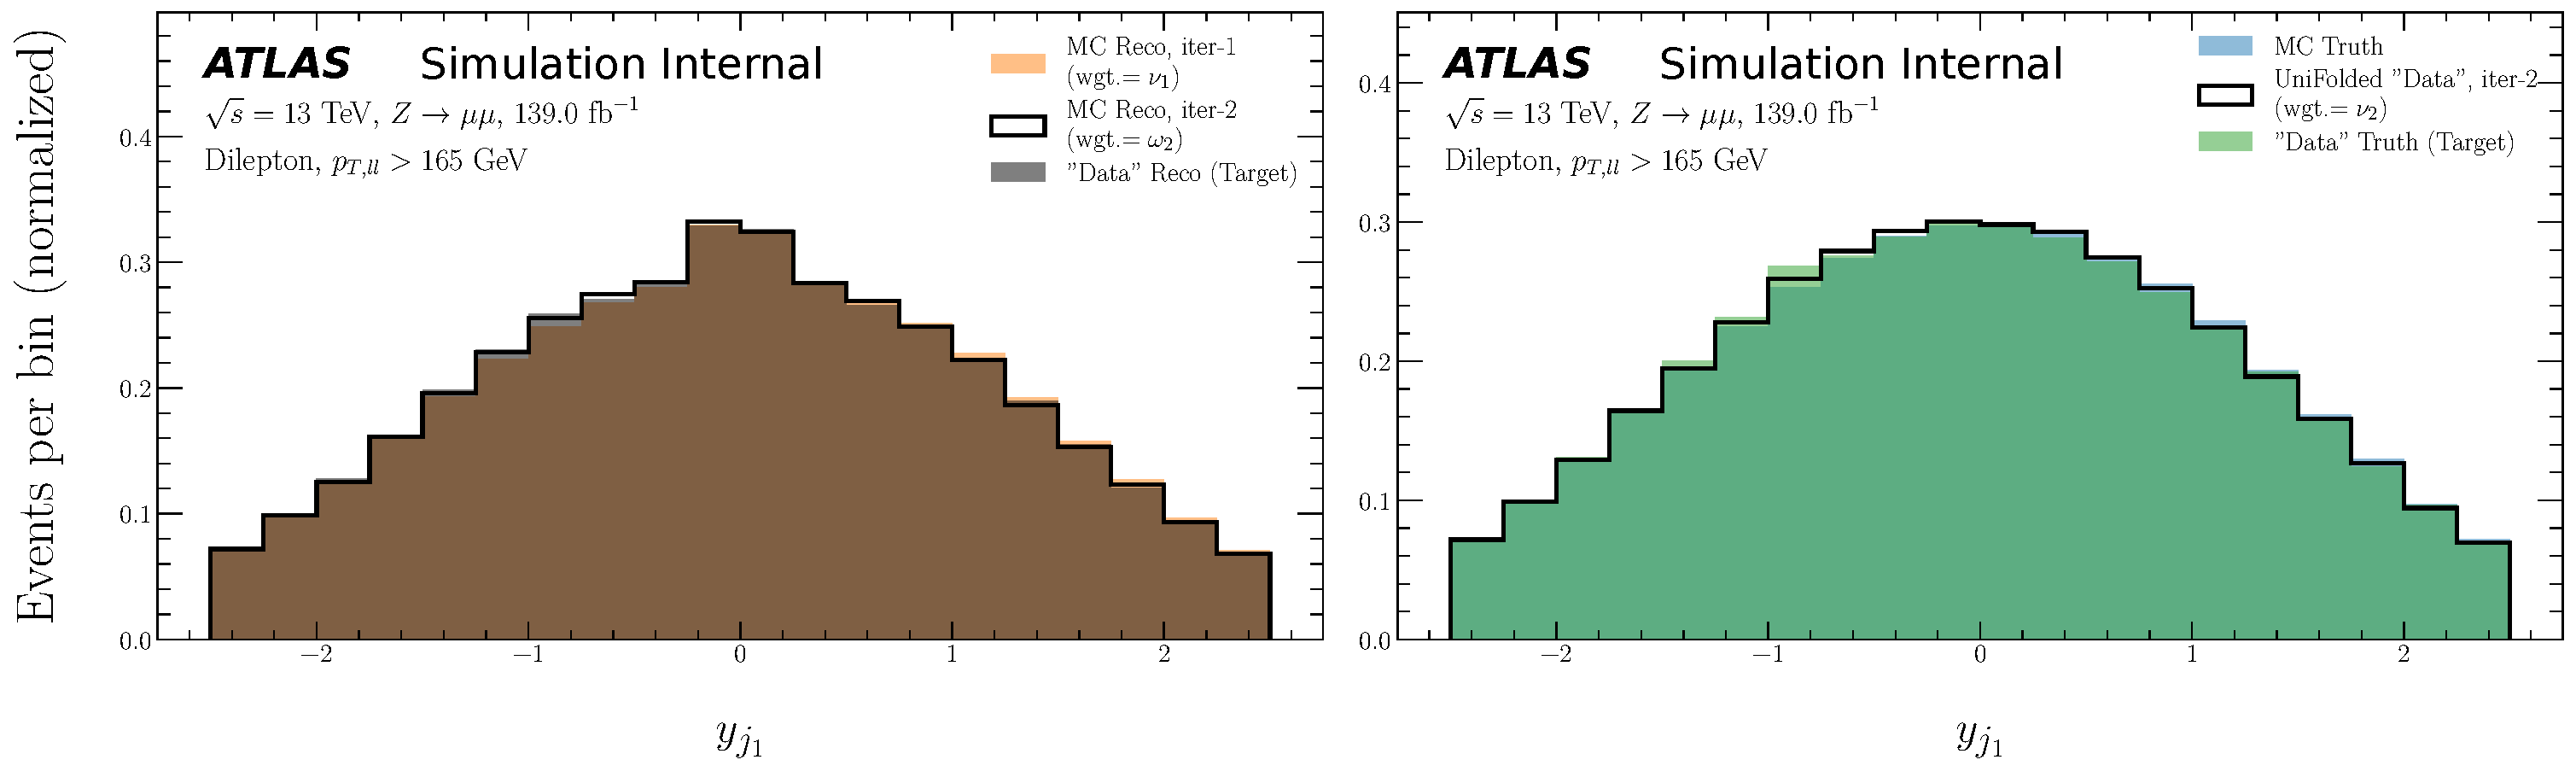
\includegraphics[width=0.85\textwidth]{figures/ATLASOmniFold-StressTest/ATLASOmniFold-StressTestC/UniFold/y_trackj1/ATLASOmniFold-StressTestC-UniFold-y_trackj1-Iteration02}}
\phantomcaption 
\end{figure}

\begin{figure}[h!]
\centering
\ContinuedFloat
\subfloat[After 3 iterations]{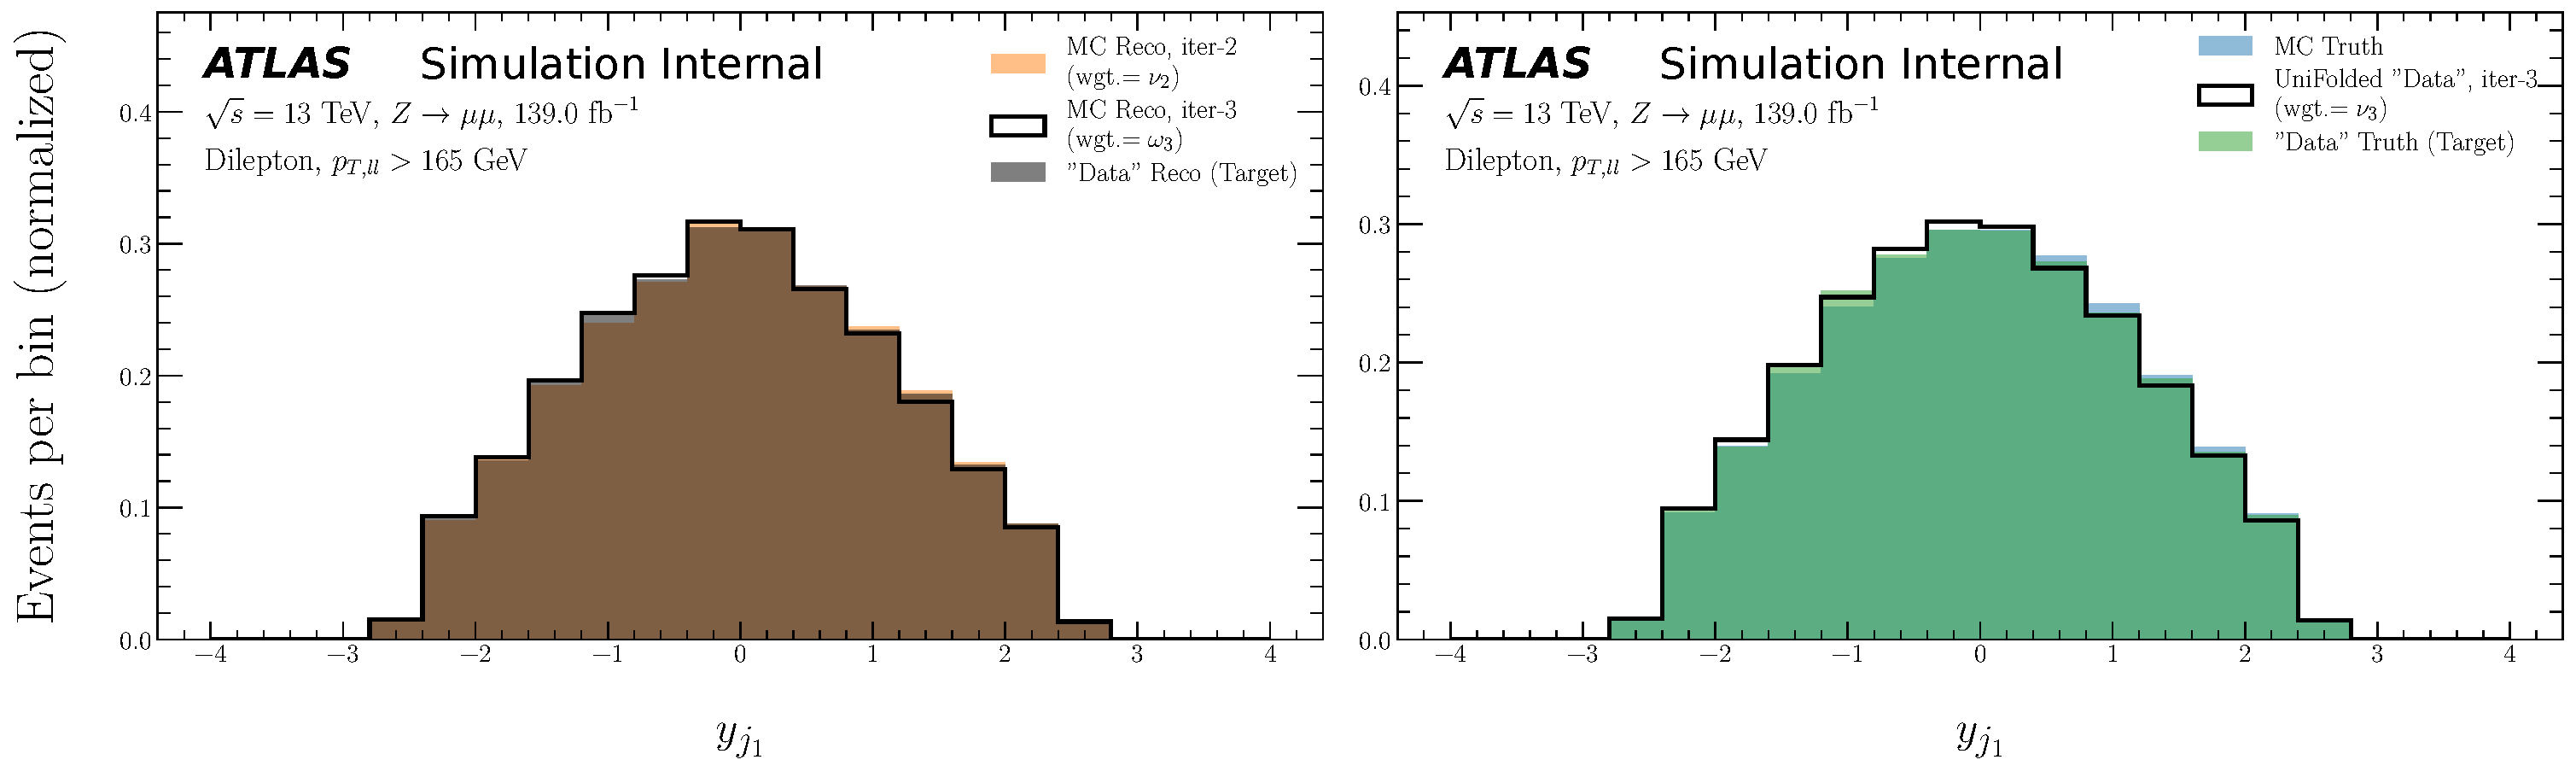
\includegraphics[width=0.85\textwidth]{figures/ATLASOmniFold-StressTest/ATLASOmniFold-StressTestC/UniFold/y_trackj1/ATLASOmniFold-StressTestC-UniFold-y_trackj1-Iteration03}}\\
\subfloat[After 4 iterations]{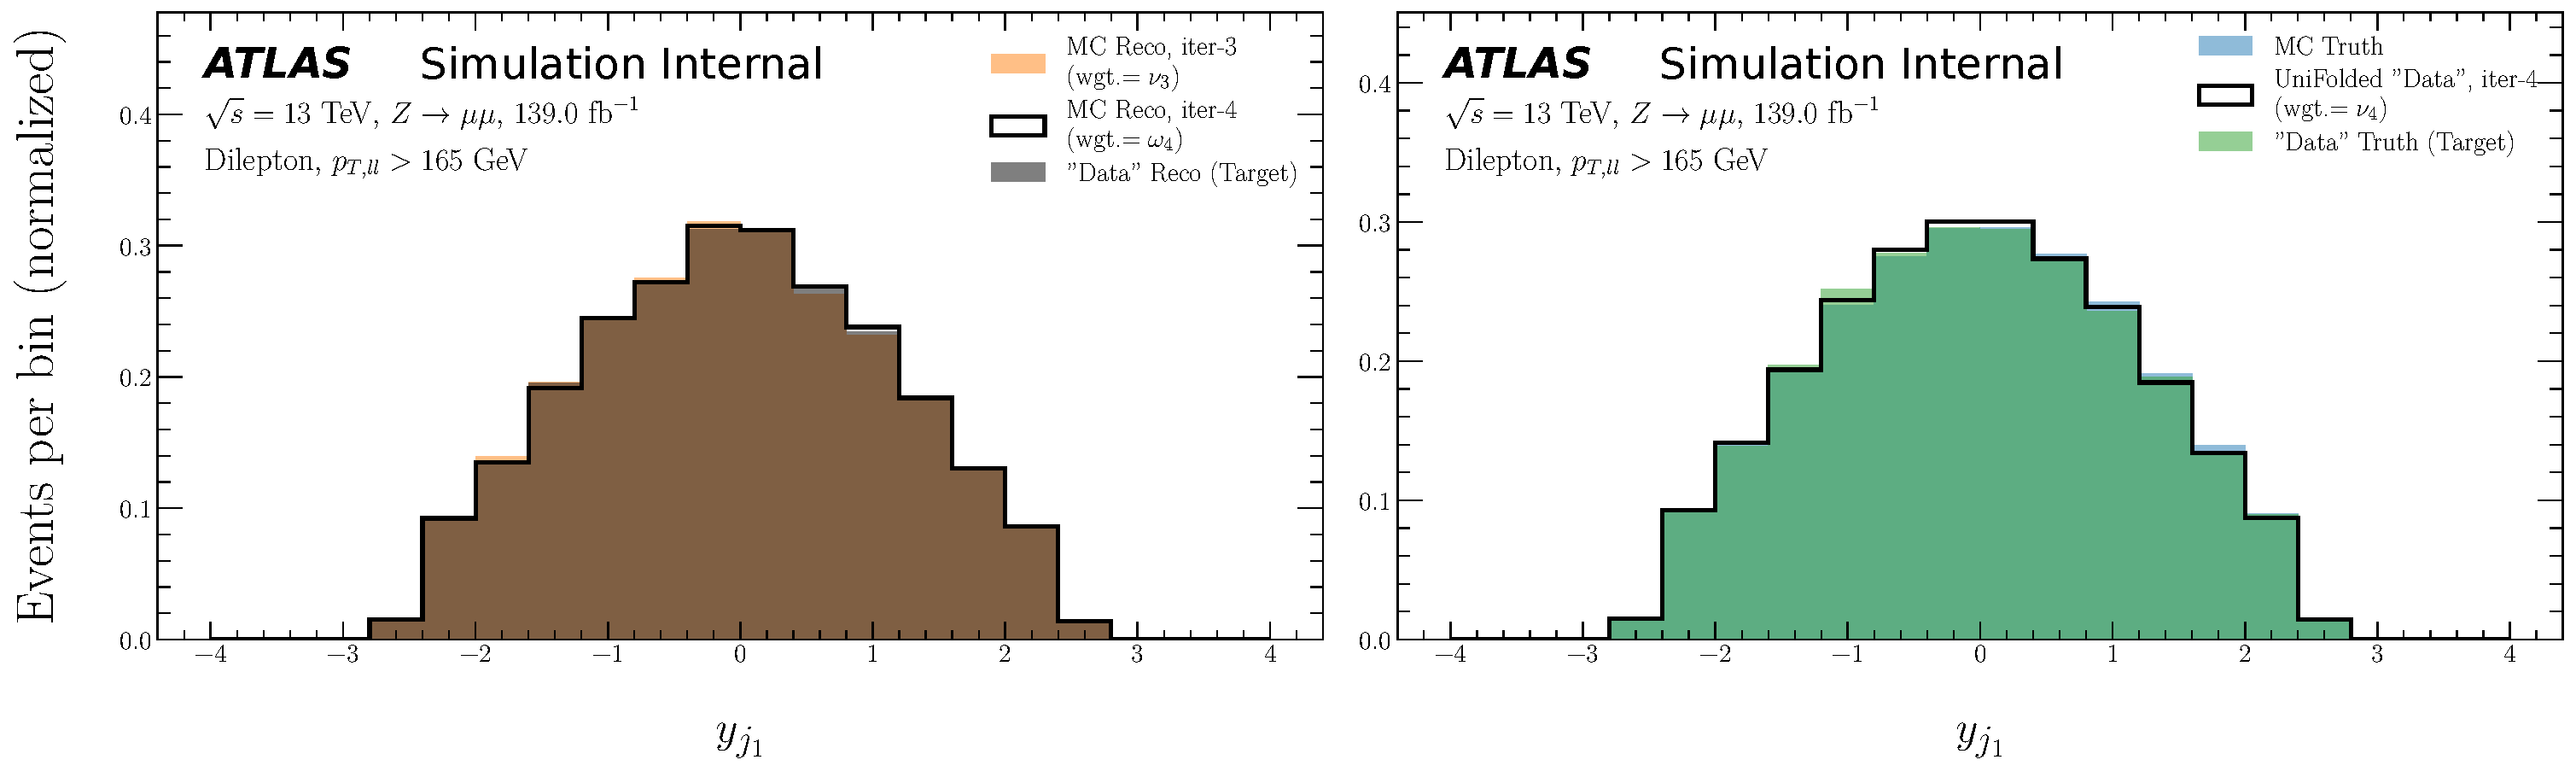
\includegraphics[width=0.85\textwidth]{figures/ATLASOmniFold-StressTest/ATLASOmniFold-StressTestC/UniFold/y_trackj1/ATLASOmniFold-StressTestC-UniFold-y_trackj1-Iteration04}}\\
\subfloat[After 5 iterations]{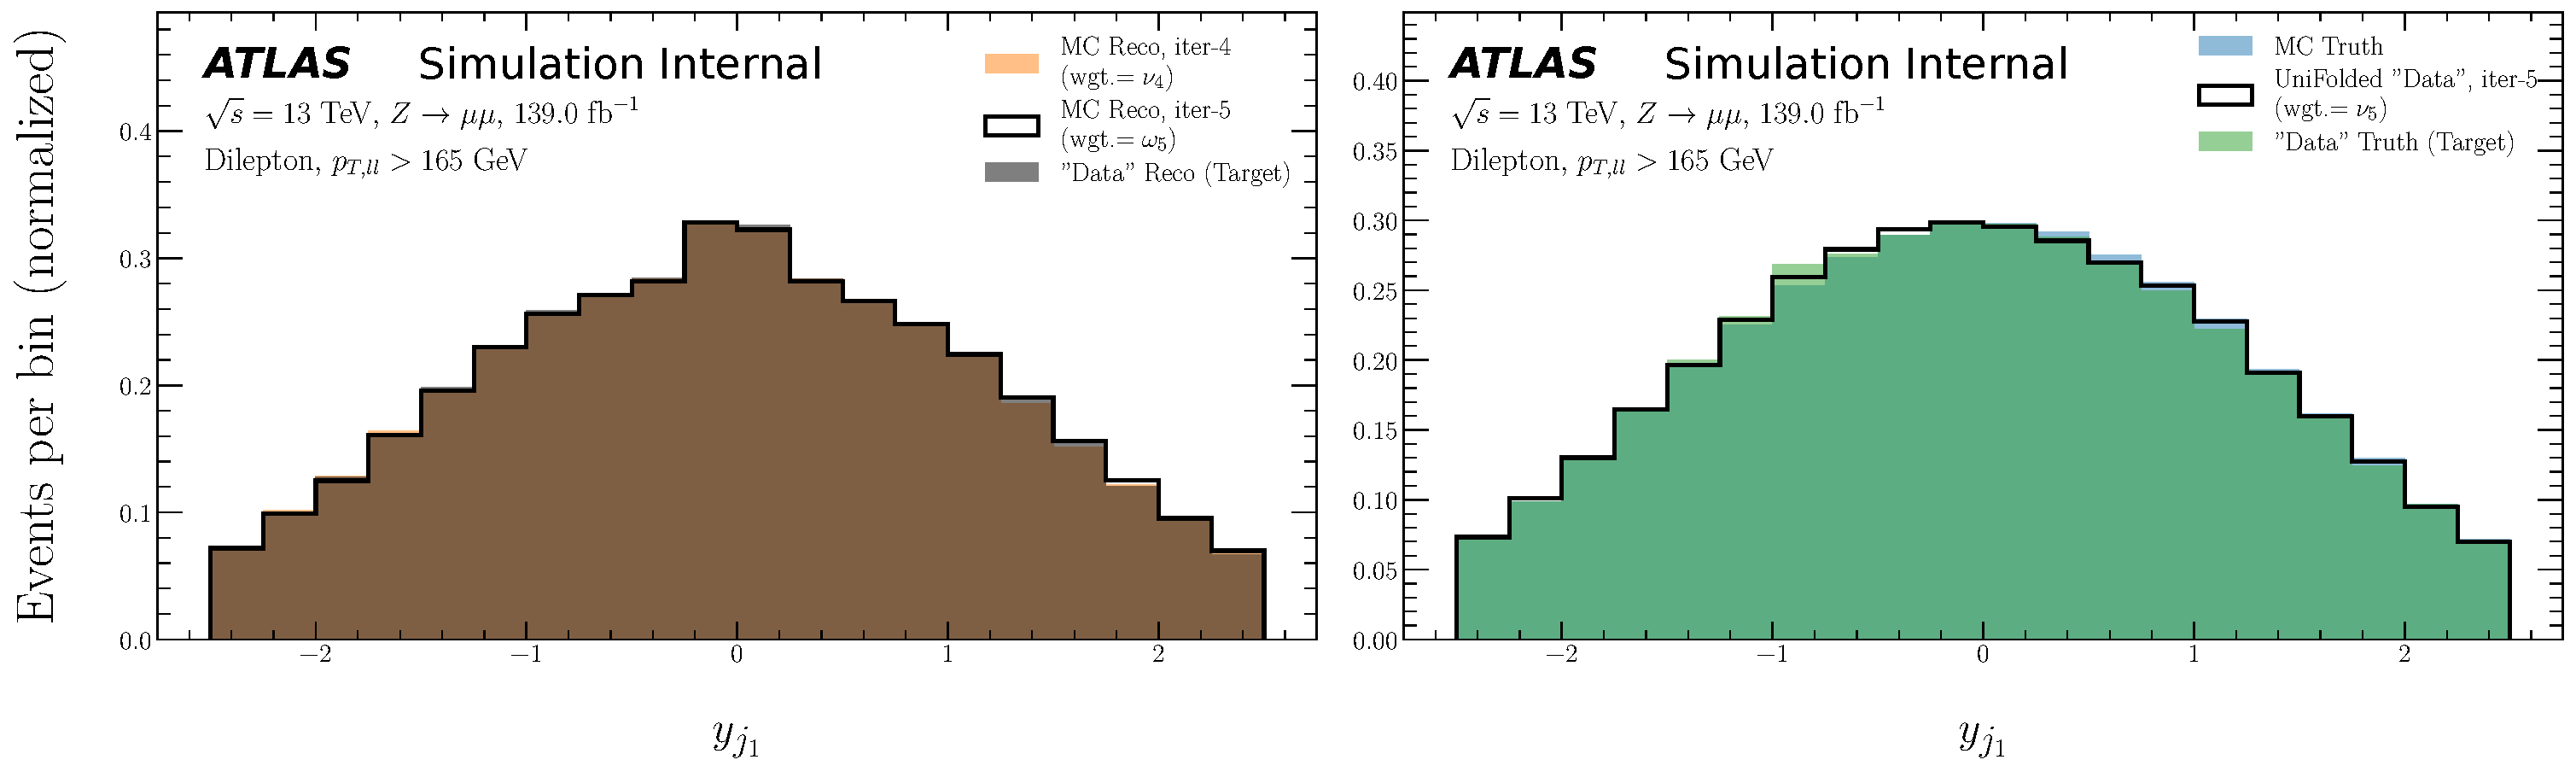
\includegraphics[width=0.85\textwidth]{figures/ATLASOmniFold-StressTest/ATLASOmniFold-StressTestC/UniFold/y_trackj1/ATLASOmniFold-StressTestC-UniFold-y_trackj1-Iteration05}}\\
\subfloat[After 6 iterations]{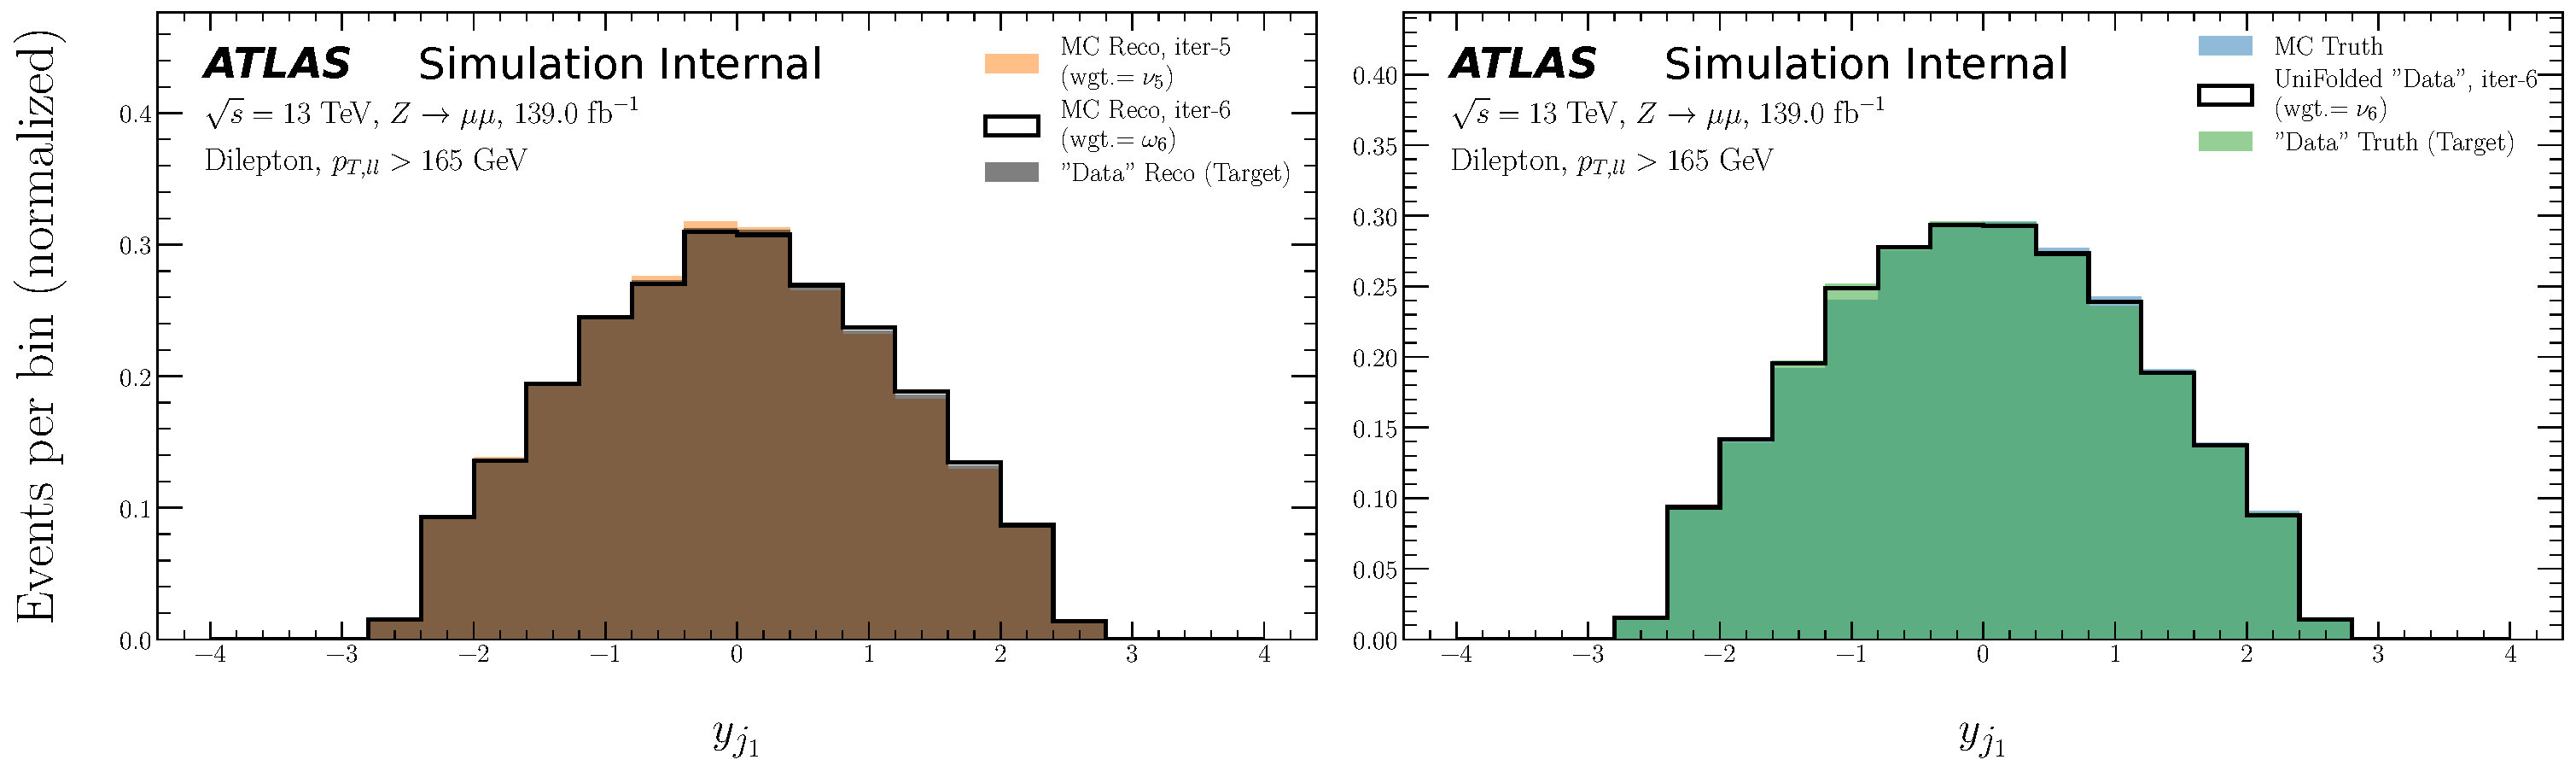
\includegraphics[width=0.85\textwidth]{figures/ATLASOmniFold-StressTest/ATLASOmniFold-StressTestC/UniFold/y_trackj1/ATLASOmniFold-StressTestC-UniFold-y_trackj1-Iteration06}}
\caption{UniFolding Sherpa with Pythia for the leading track jet rapidity.}
\label{fig:stressc_y_trackj1}
\end{figure}

\section{Model dependence for MultiFold}
\label{sec:stresscmultifolddet} 

Following from Sec.~\ref{sec:modeldep}, Figures~\ref{fig:stressc_pT_trackj1Multi},~\ref{fig:stressc_y_trackj1Multi},~\ref{fig:stressc_tau1_trackj1Multi},~\ref{fig:stressc_tau2_trackj1Multi},~\ref{fig:stressc_tau3_trackj1Multi}, show the MultiFold results for the properties of the leading track jet, Figs.~\ref{fig:stressc_massMulti},~\ref{fig:stressc_Ntracks_trackj2Multi},~\ref{fig:stressc_pT_trackj2Multi},~\ref{fig:stressc_y_trackj2Multi},~\ref{fig:stressc_tau1_trackj2Multi},~\ref{fig:stressc_tau2_trackj2Multi},~\ref{fig:stressc_tau3_trackj2Multi} show the unfolded properties of the subleading track jet and Fig.~\ref{fig:stressc_pT_llMulti} and Fig.~\ref{fig:stressc_y_llMulti} for the dilepton properties.

\begin{figure}[h!]
\centering
\subfloat[Input histograms]{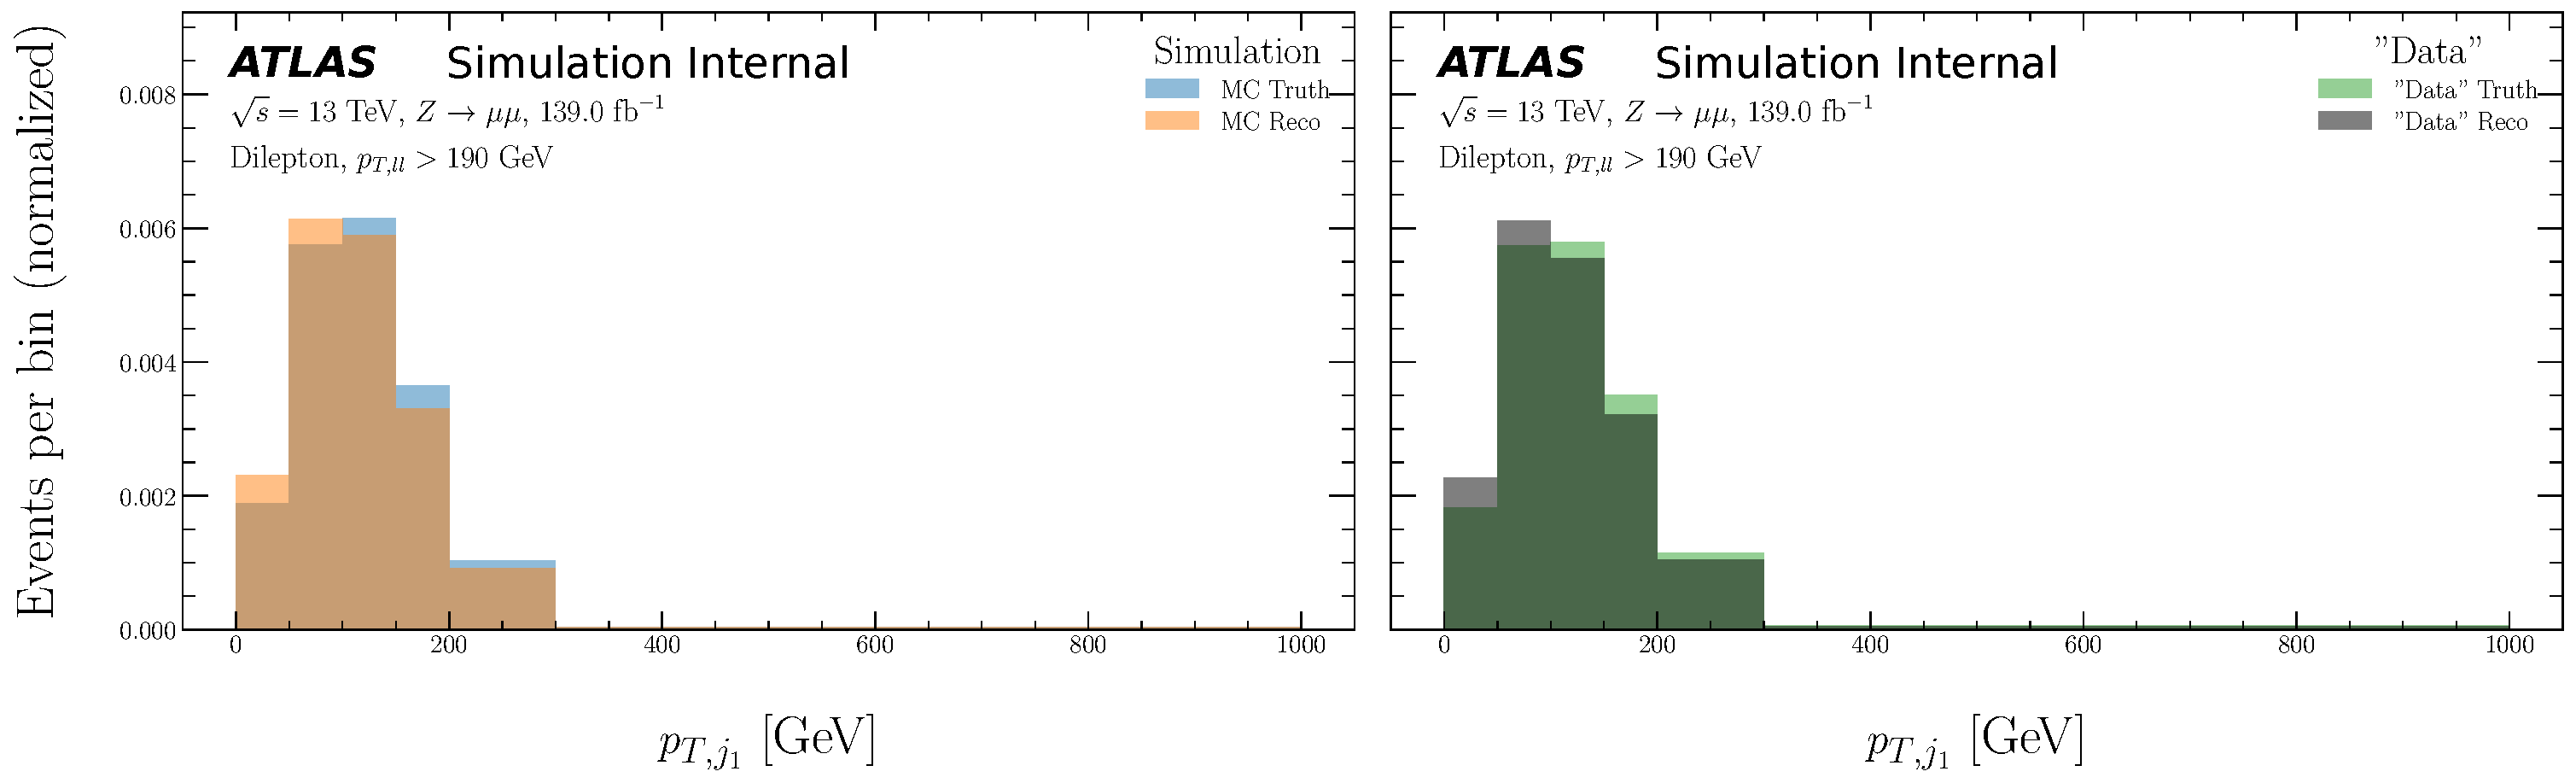
\includegraphics[width=0.85\textwidth]{figures/ATLASOmniFold-StressTest/ATLASOmniFold-StressTestC/MultiFold/pT_trackj1/ATLASOmniFold-StressTestC-MultiFold-pT_trackj1-Distributions}}\\
\subfloat[After 1 iteration]{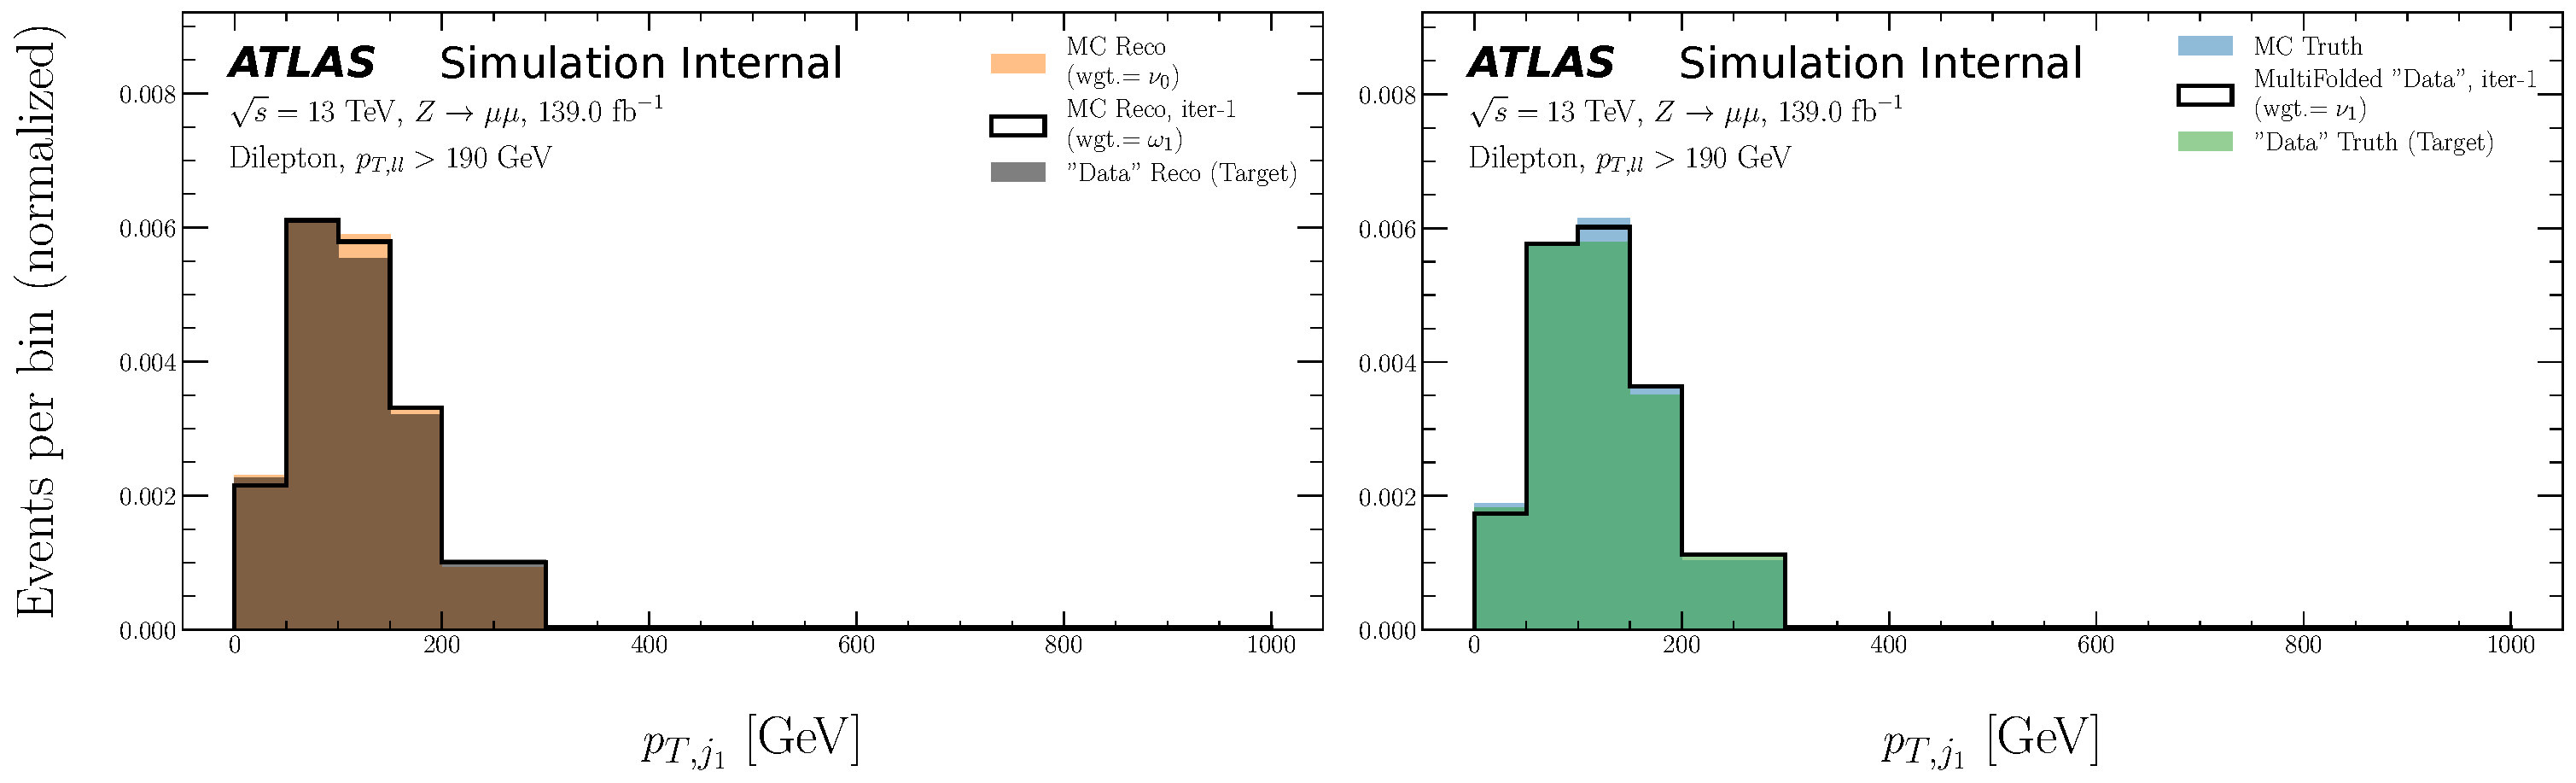
\includegraphics[width=0.85\textwidth]{figures/ATLASOmniFold-StressTest/ATLASOmniFold-StressTestC/MultiFold/pT_trackj1/ATLASOmniFold-StressTestC-MultiFold-pT_trackj1-Iteration01}}\\
\subfloat[After 2 iterations]{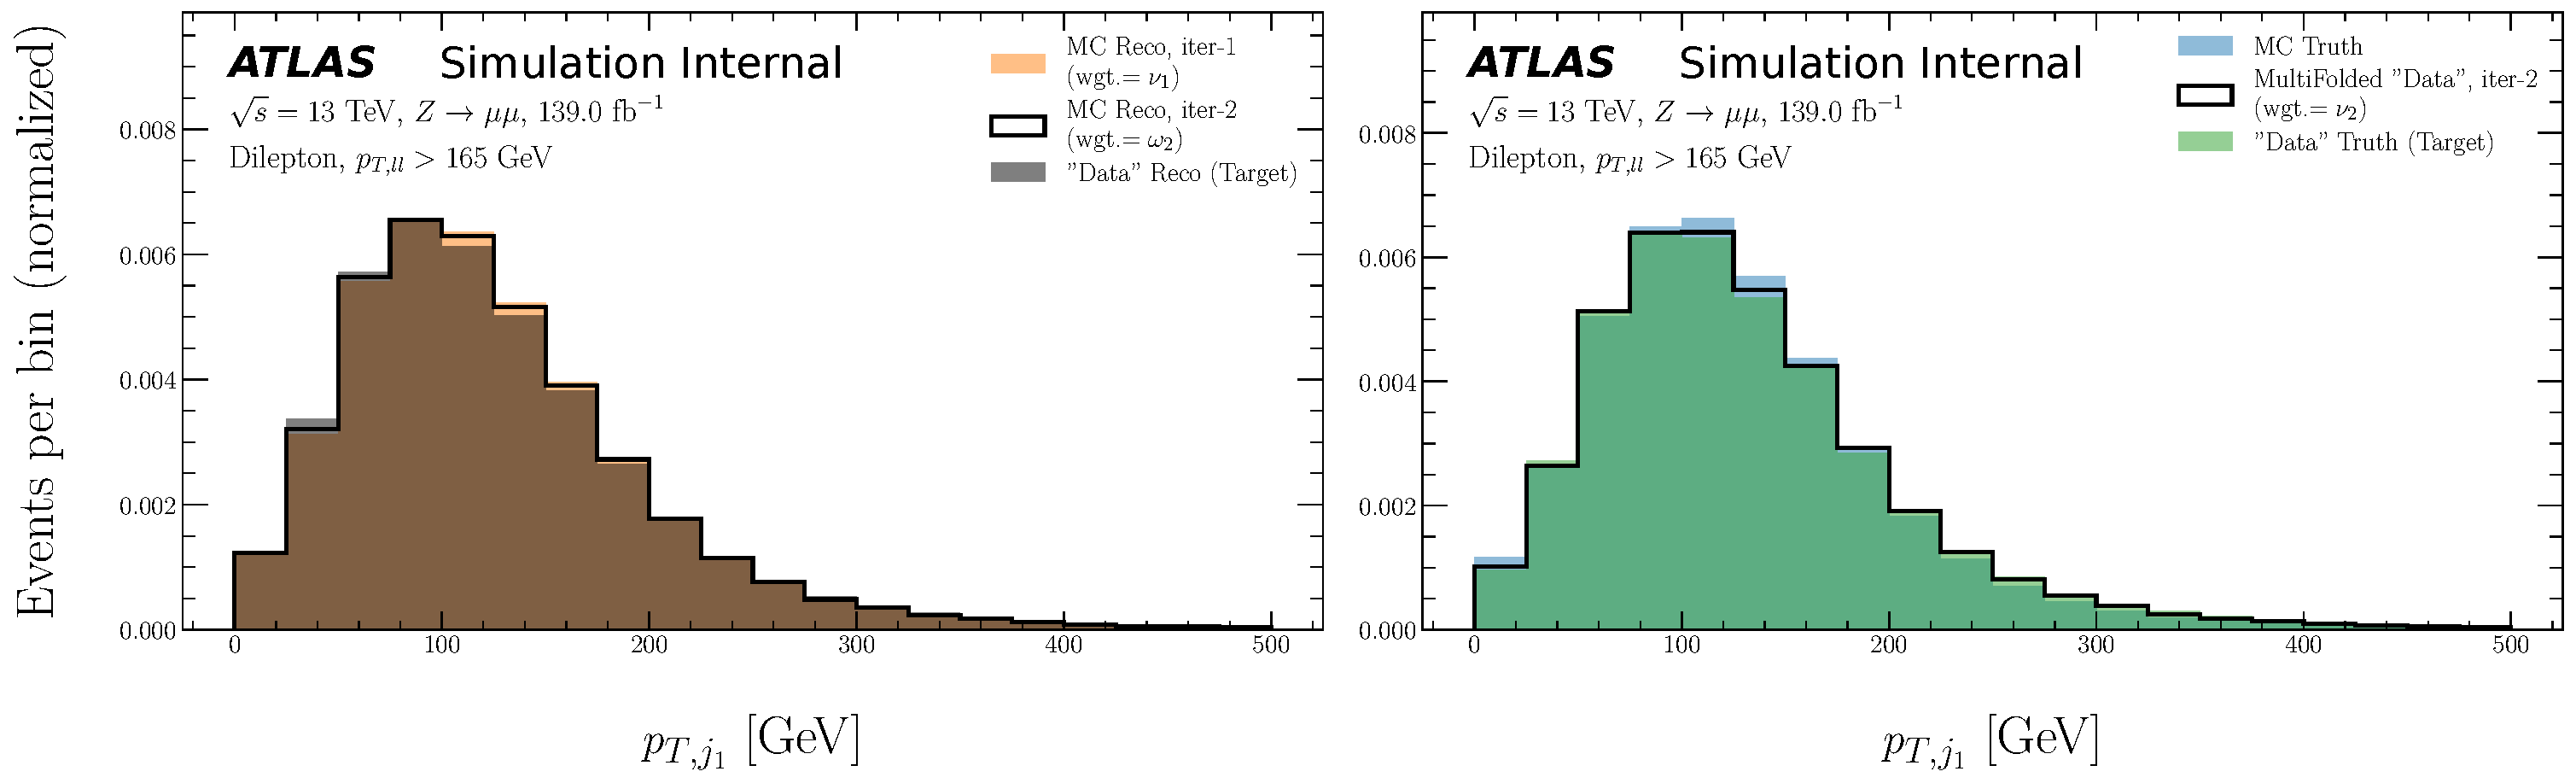
\includegraphics[width=0.85\textwidth]{figures/ATLASOmniFold-StressTest/ATLASOmniFold-StressTestC/MultiFold/pT_trackj1/ATLASOmniFold-StressTestC-MultiFold-pT_trackj1-Iteration02}}
\phantomcaption 
\end{figure}

\begin{figure}[h!]
\centering
\ContinuedFloat
\subfloat[After 3 iterations]{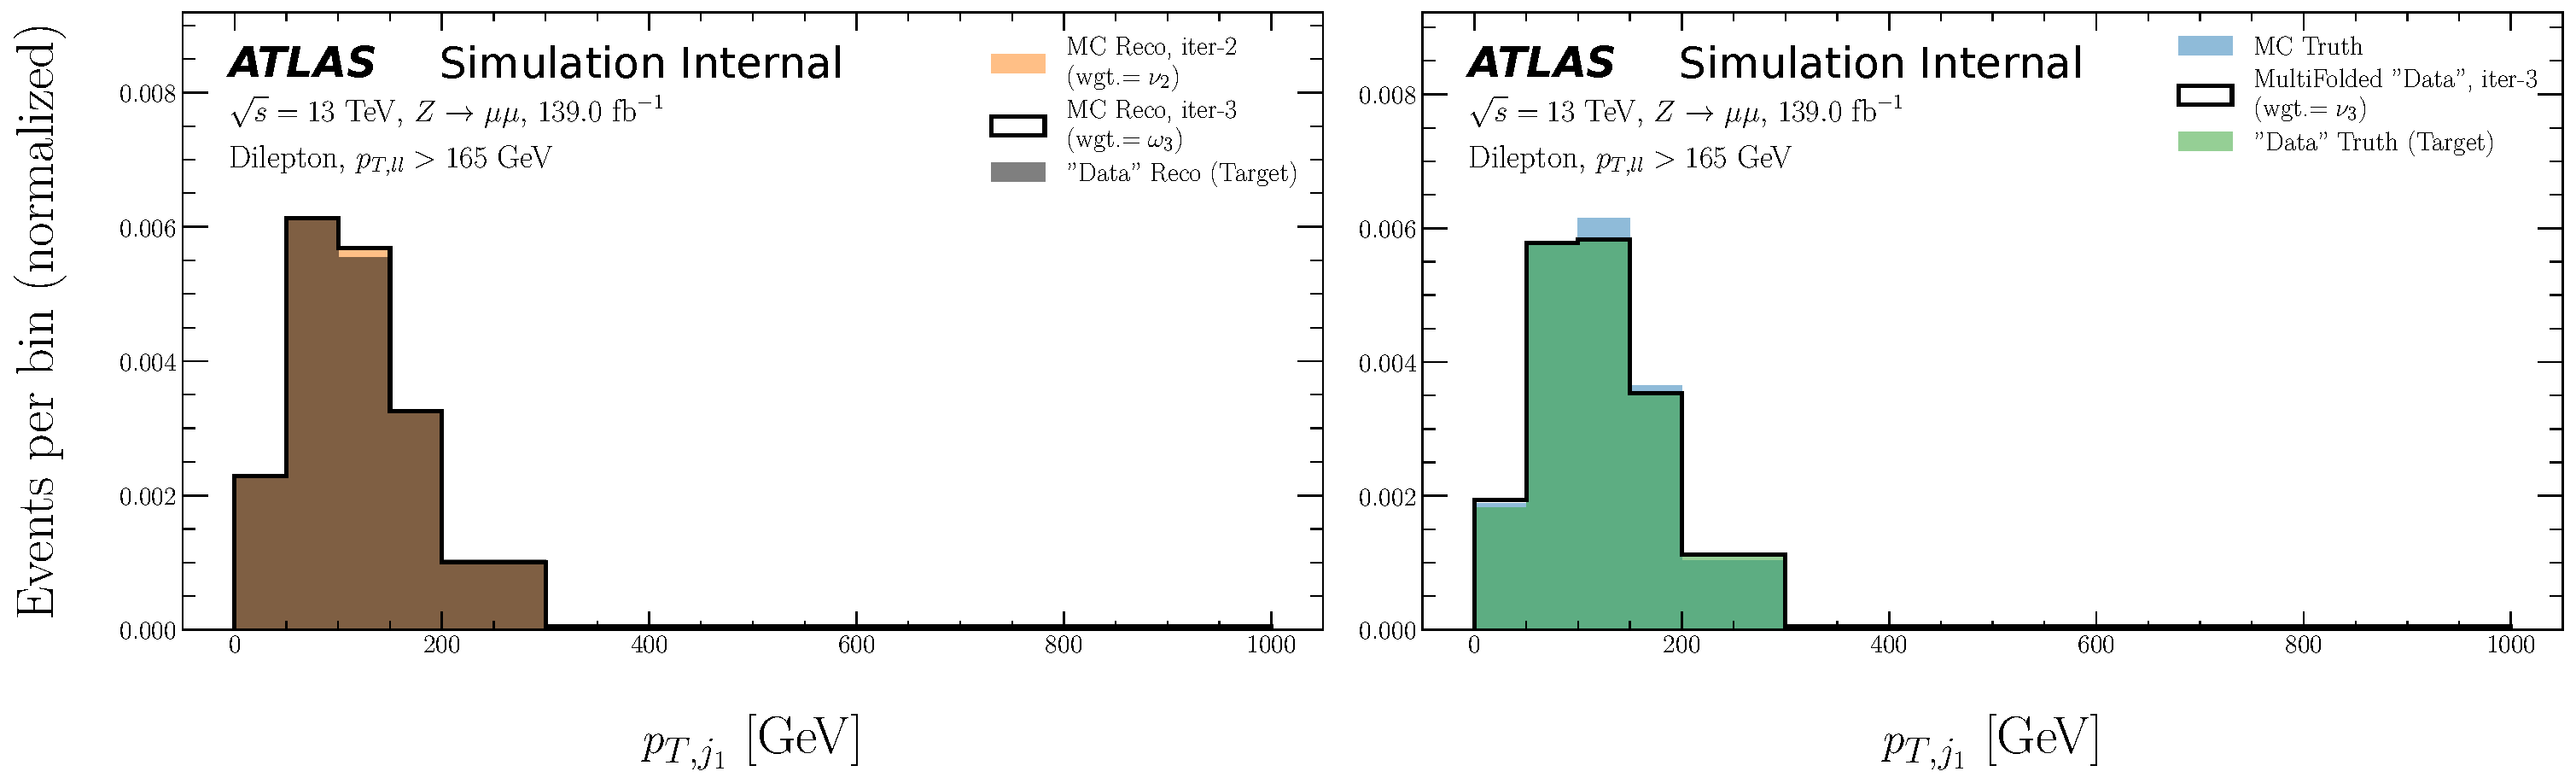
\includegraphics[width=0.85\textwidth]{figures/ATLASOmniFold-StressTest/ATLASOmniFold-StressTestC/MultiFold/pT_trackj1/ATLASOmniFold-StressTestC-MultiFold-pT_trackj1-Iteration03}}\\
\subfloat[After 4 iterations]{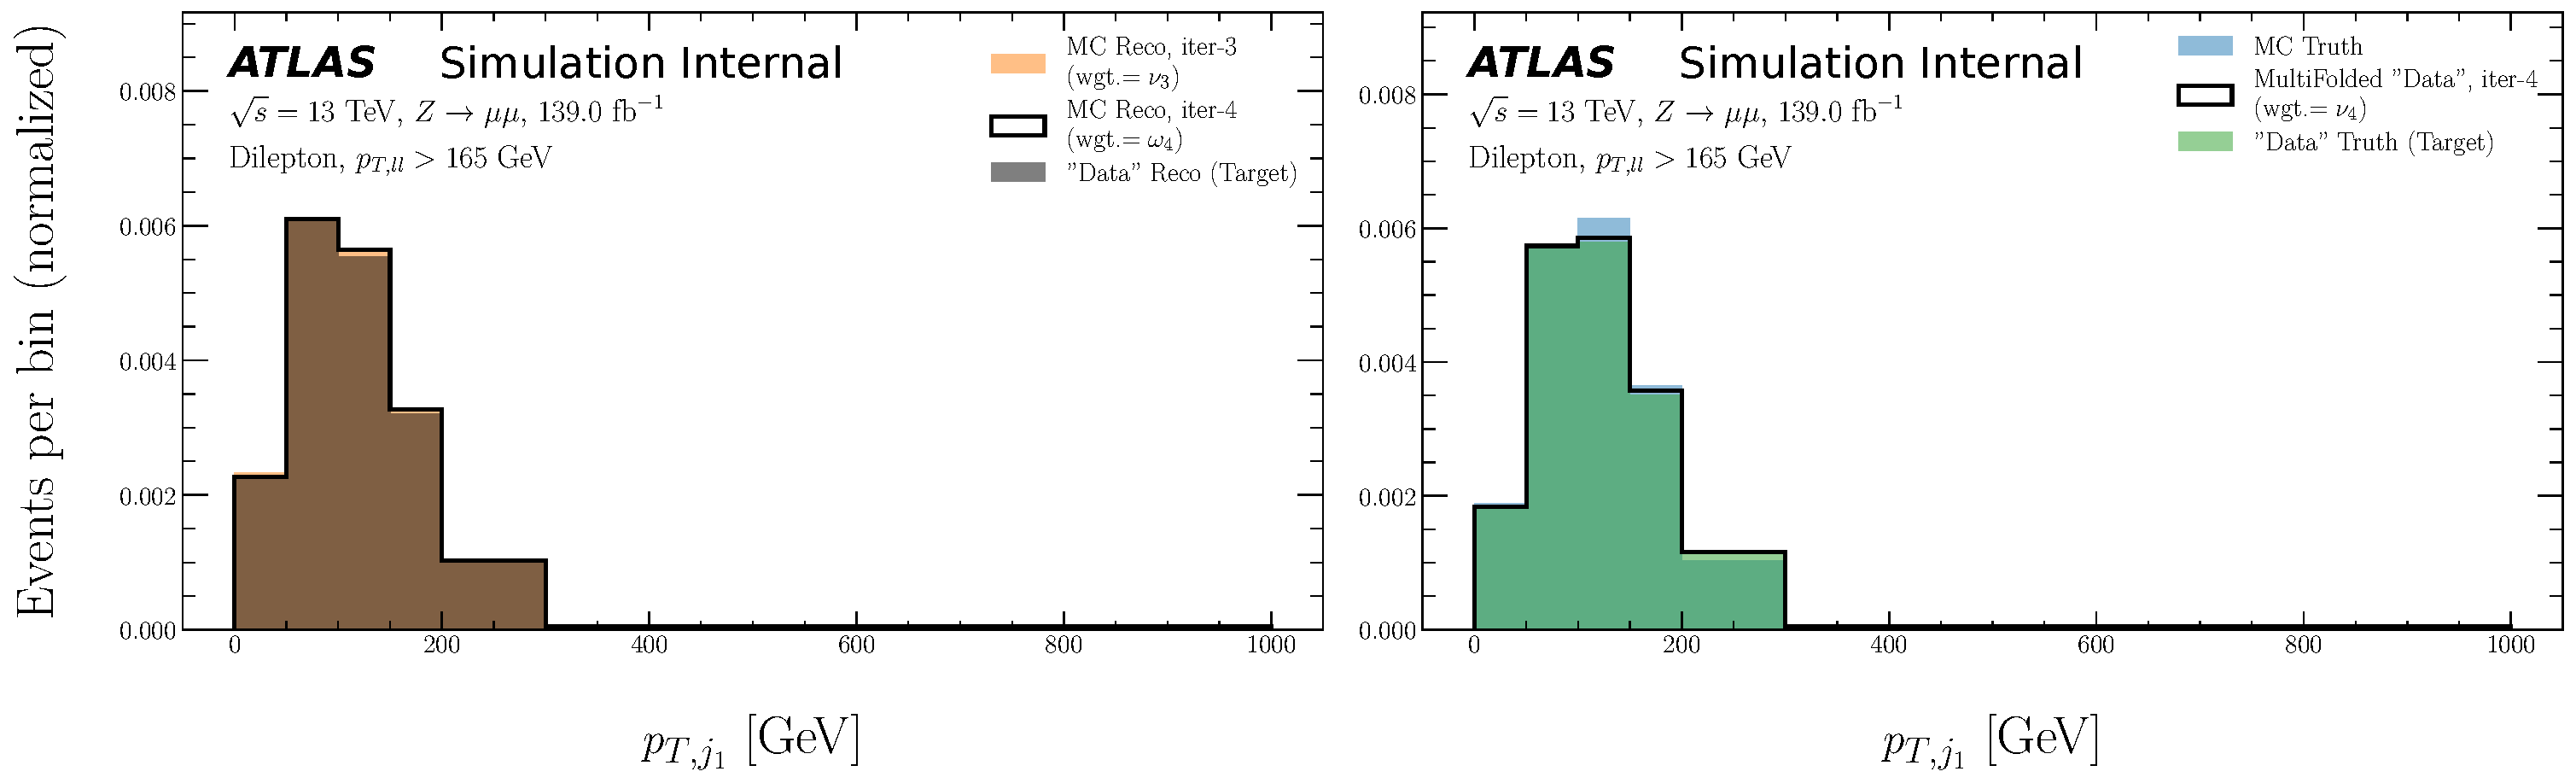
\includegraphics[width=0.85\textwidth]{figures/ATLASOmniFold-StressTest/ATLASOmniFold-StressTestC/MultiFold/pT_trackj1/ATLASOmniFold-StressTestC-MultiFold-pT_trackj1-Iteration04}}\\
\subfloat[After 5 iterations]{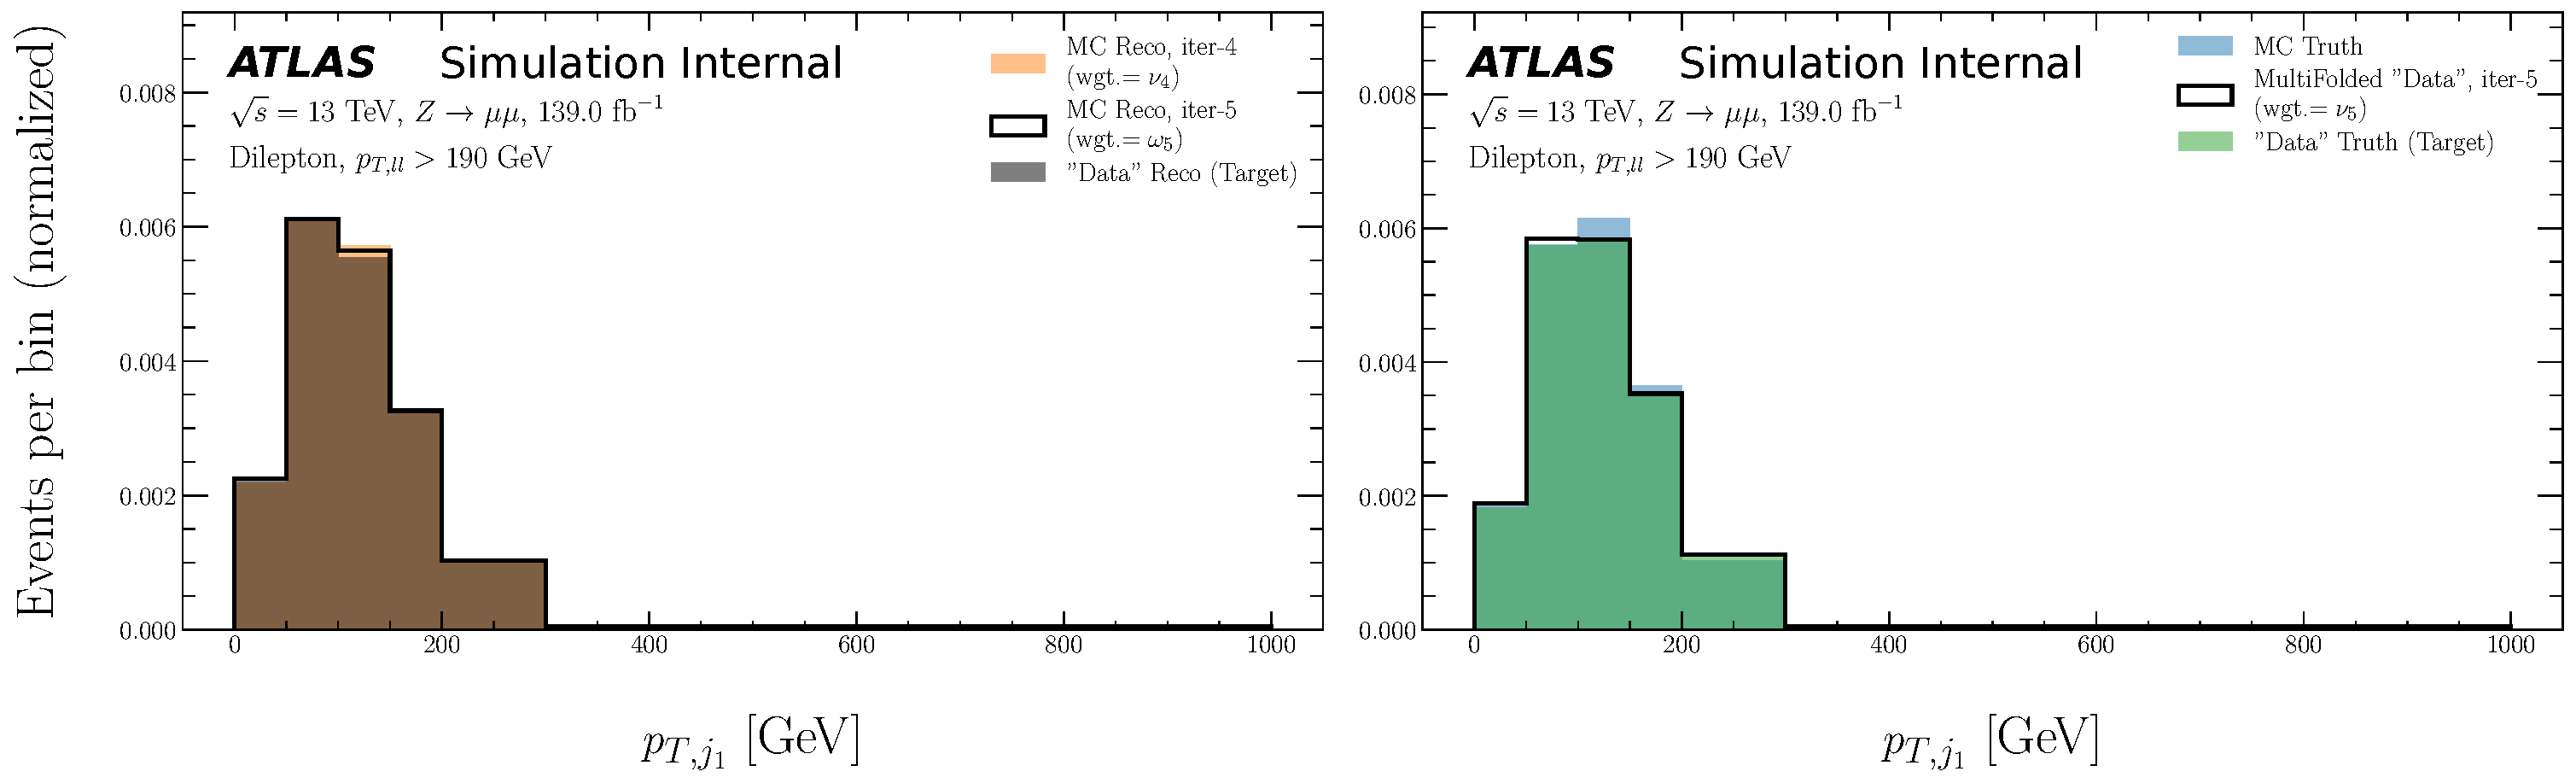
\includegraphics[width=0.85\textwidth]{figures/ATLASOmniFold-StressTest/ATLASOmniFold-StressTestC/MultiFold/pT_trackj1/ATLASOmniFold-StressTestC-MultiFold-pT_trackj1-Iteration05}}\\
\subfloat[After 6 iterations]{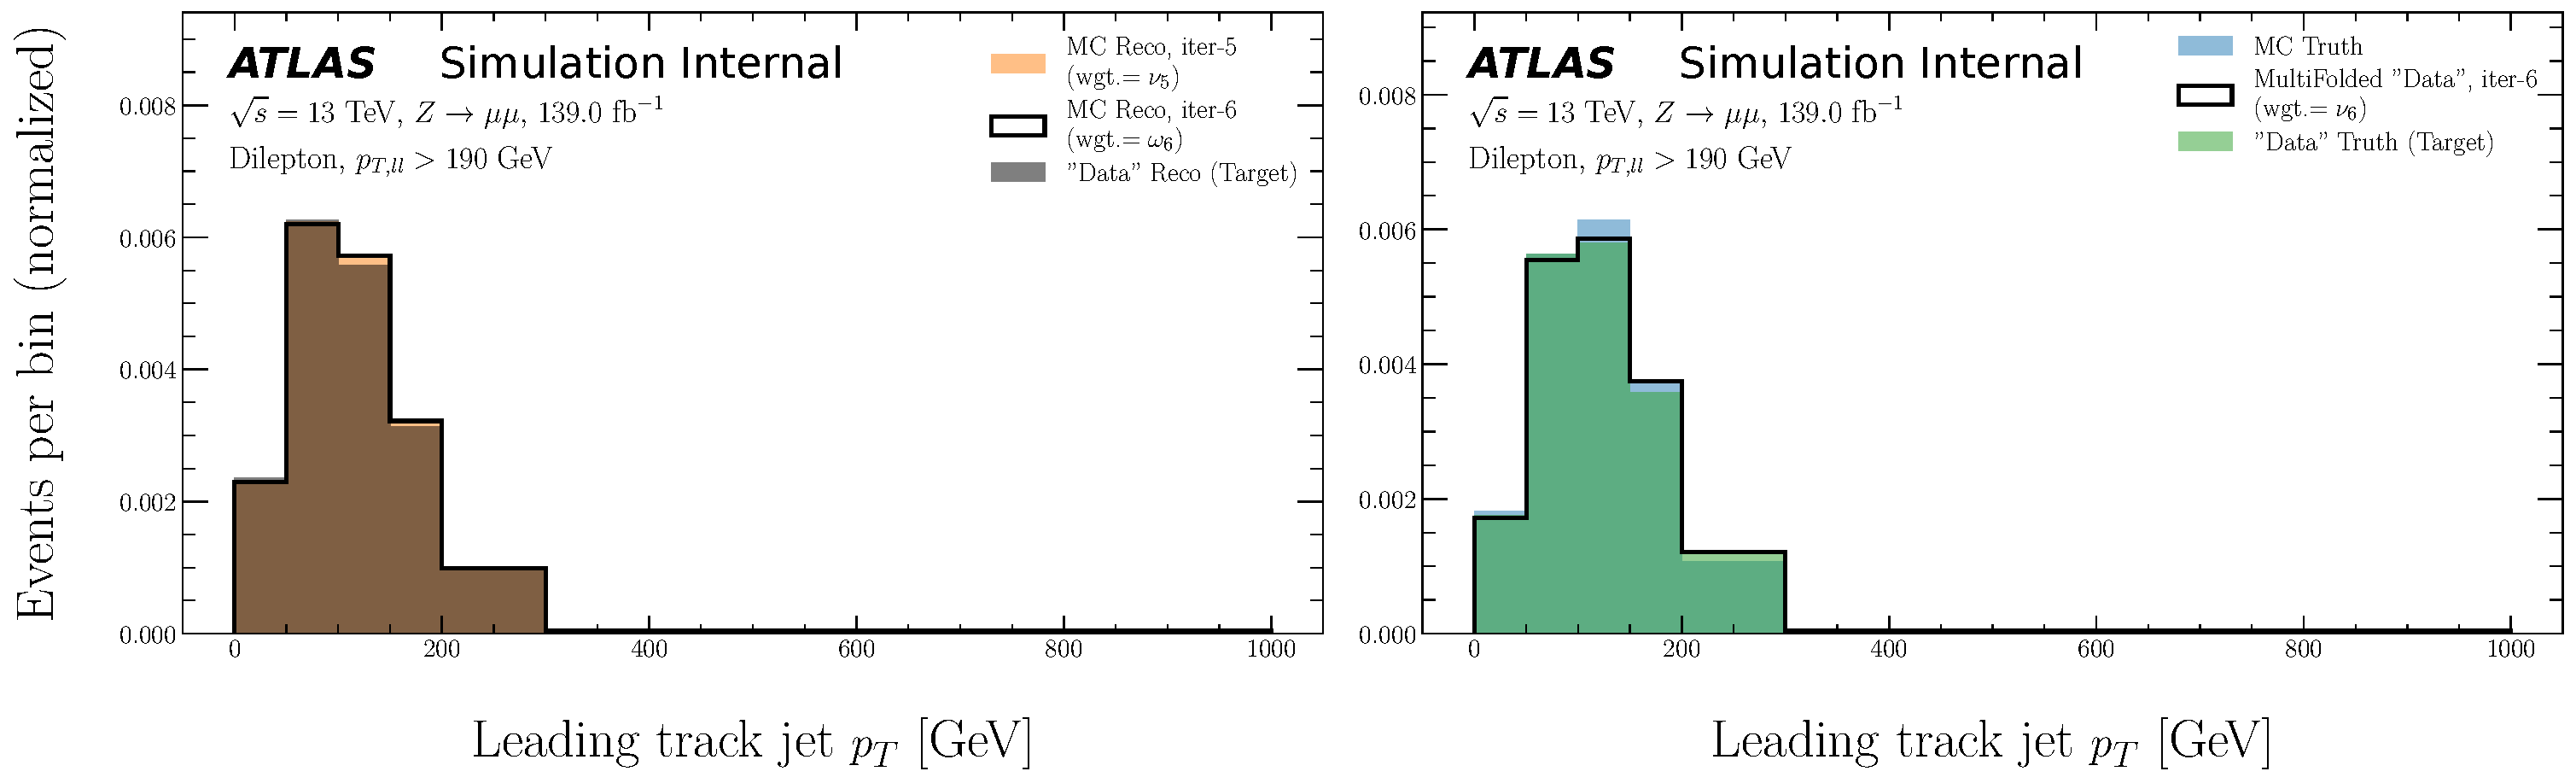
\includegraphics[width=0.85\textwidth]{figures/ATLASOmniFold-StressTest/ATLASOmniFold-StressTestC/MultiFold/pT_trackj1/ATLASOmniFold-StressTestC-MultiFold-pT_trackj1-Iteration06}}
\caption{MultiFolding Sherpa with Pythia for the leading track jet $p_T$.}
\label{fig:stressc_pT_trackj1Multi}
\end{figure}

\begin{figure}[h!]
\centering
\subfloat[Input histograms]{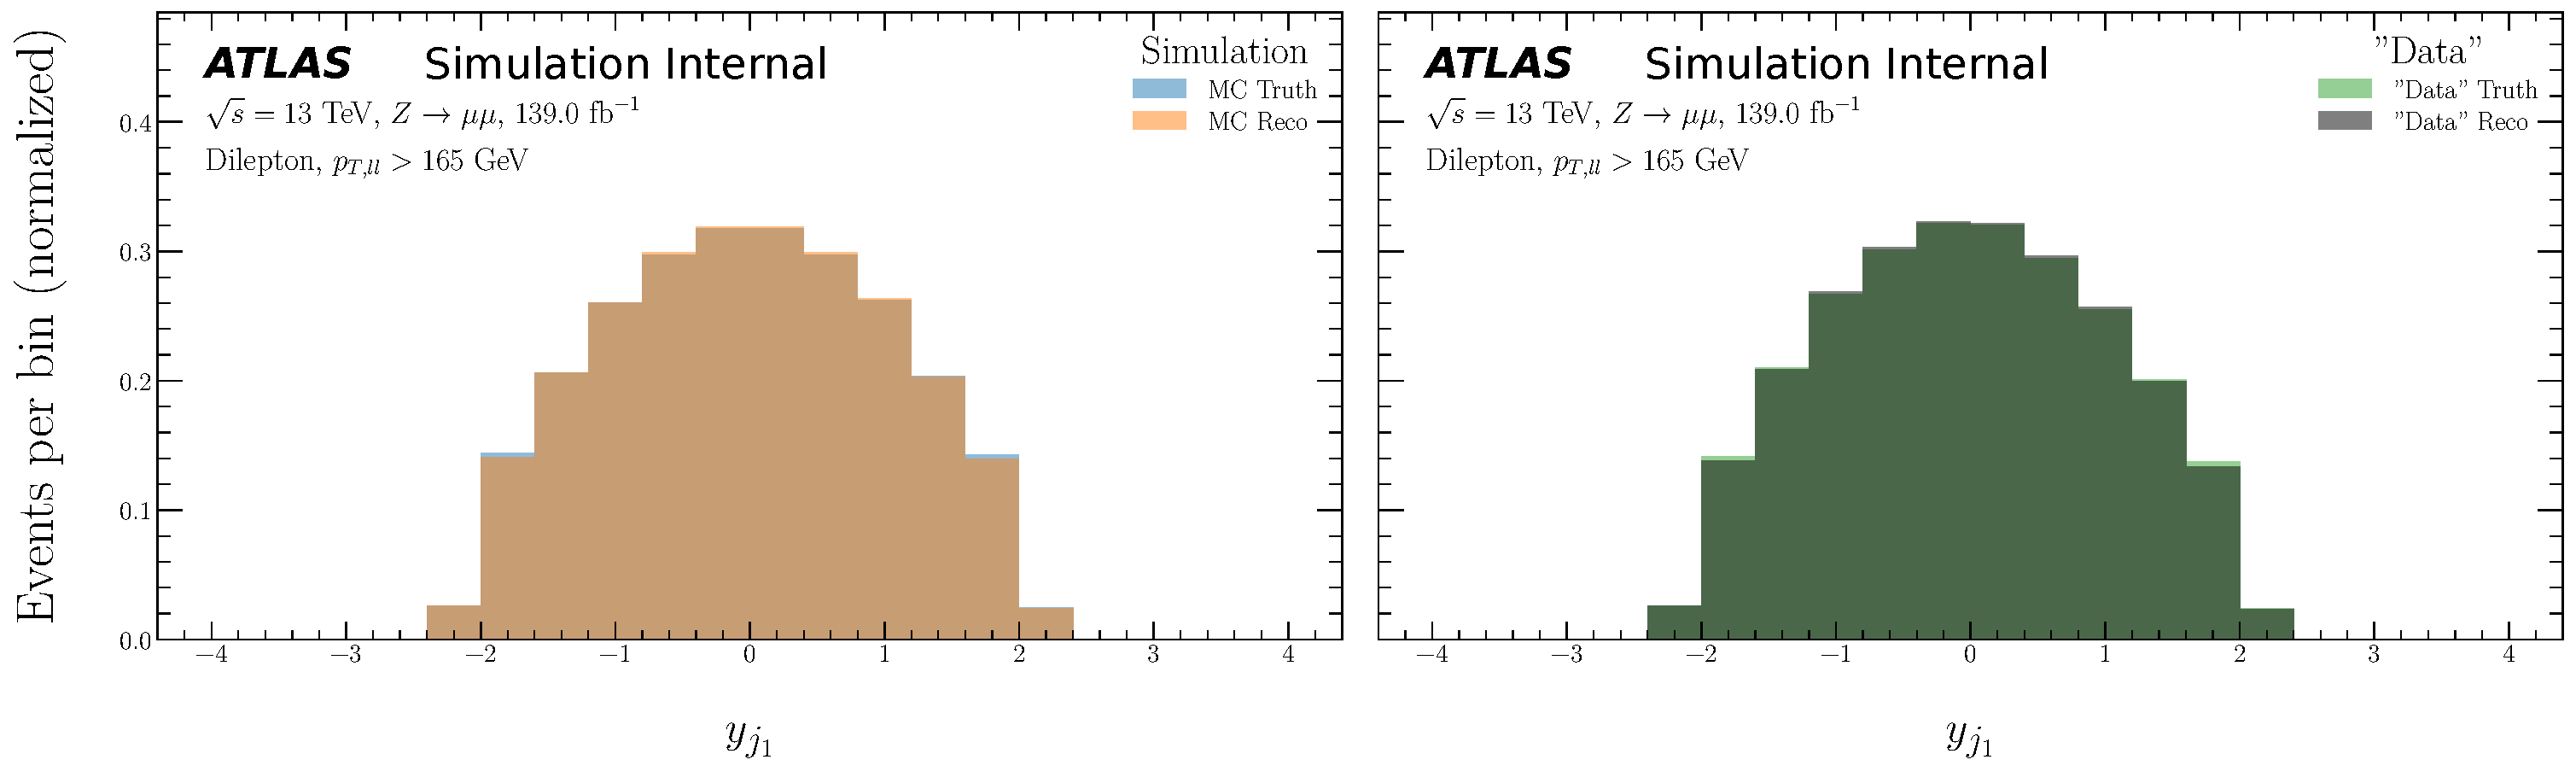
\includegraphics[width=0.85\textwidth]{figures/ATLASOmniFold-StressTest/ATLASOmniFold-StressTestC/MultiFold/y_trackj1/ATLASOmniFold-StressTestC-MultiFold-y_trackj1-Distributions}}\\
\subfloat[After 1 iteration]{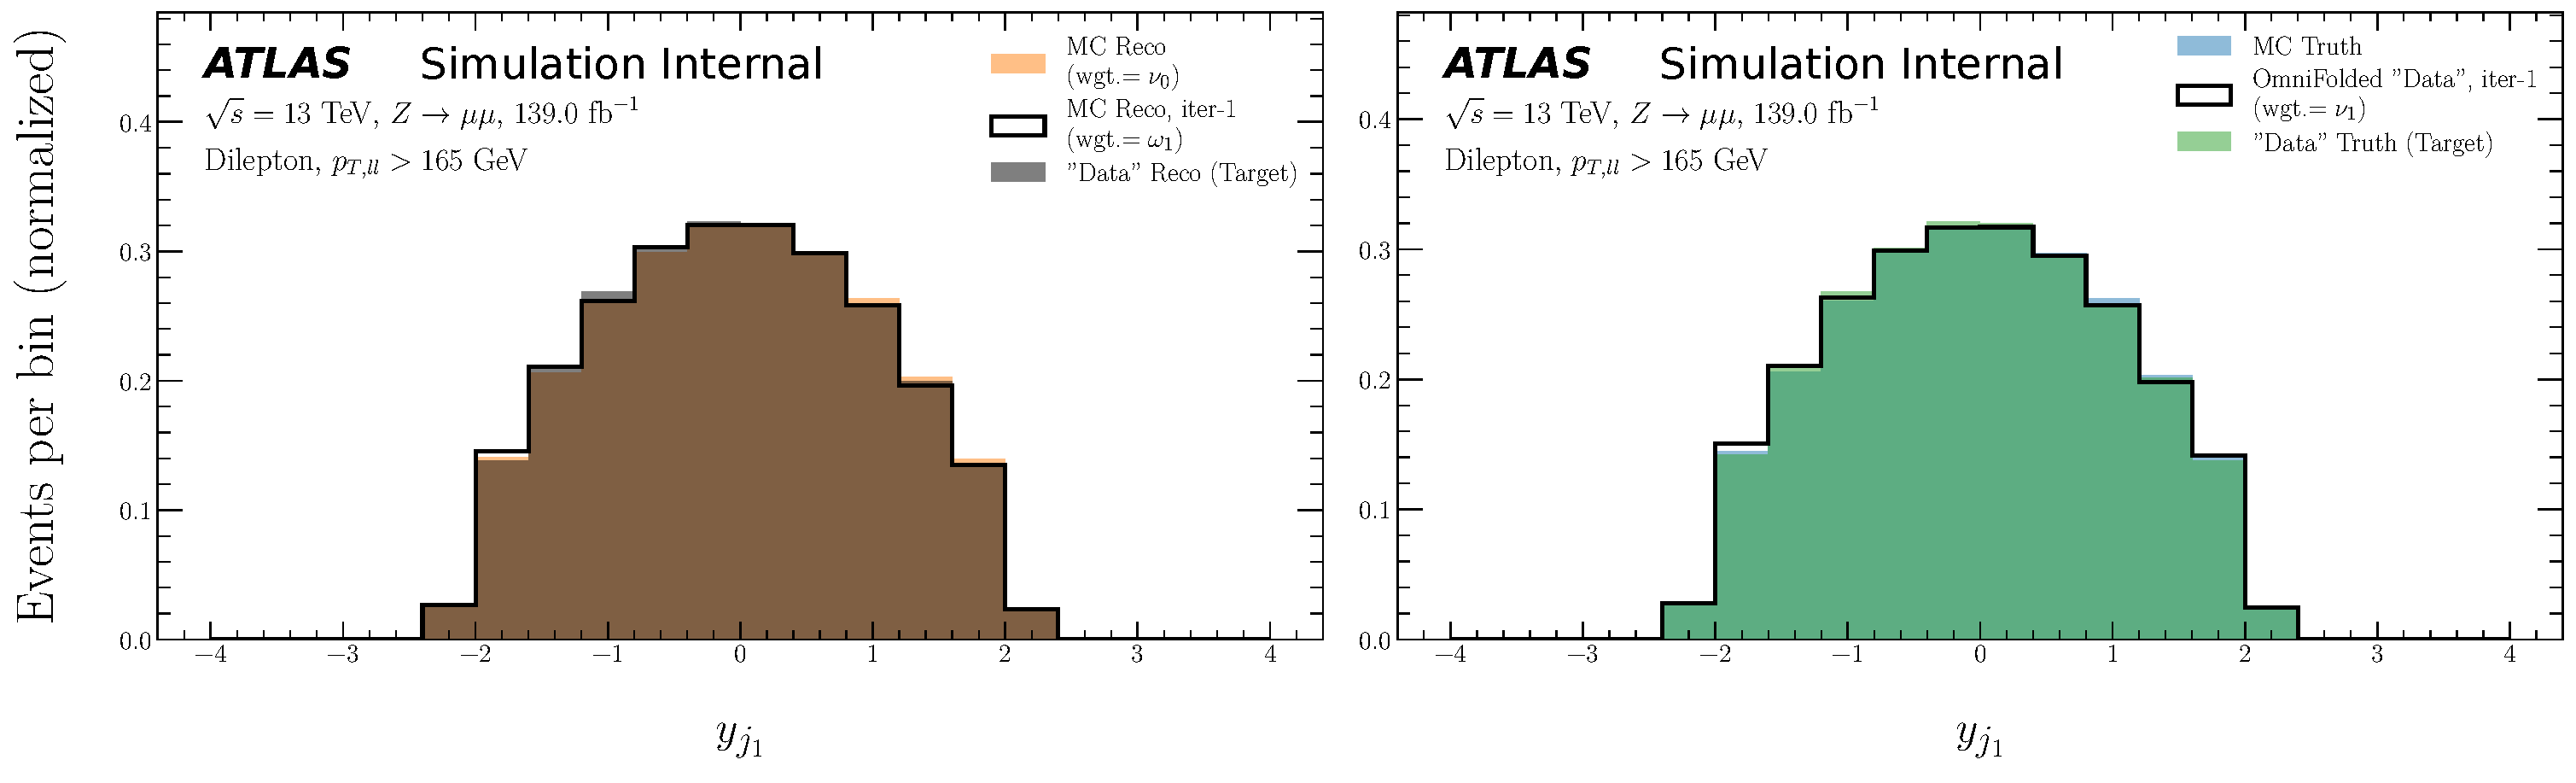
\includegraphics[width=0.85\textwidth]{figures/ATLASOmniFold-StressTest/ATLASOmniFold-StressTestC/MultiFold/y_trackj1/ATLASOmniFold-StressTestC-MultiFold-y_trackj1-Iteration01}}\\
\subfloat[After 2 iterations]{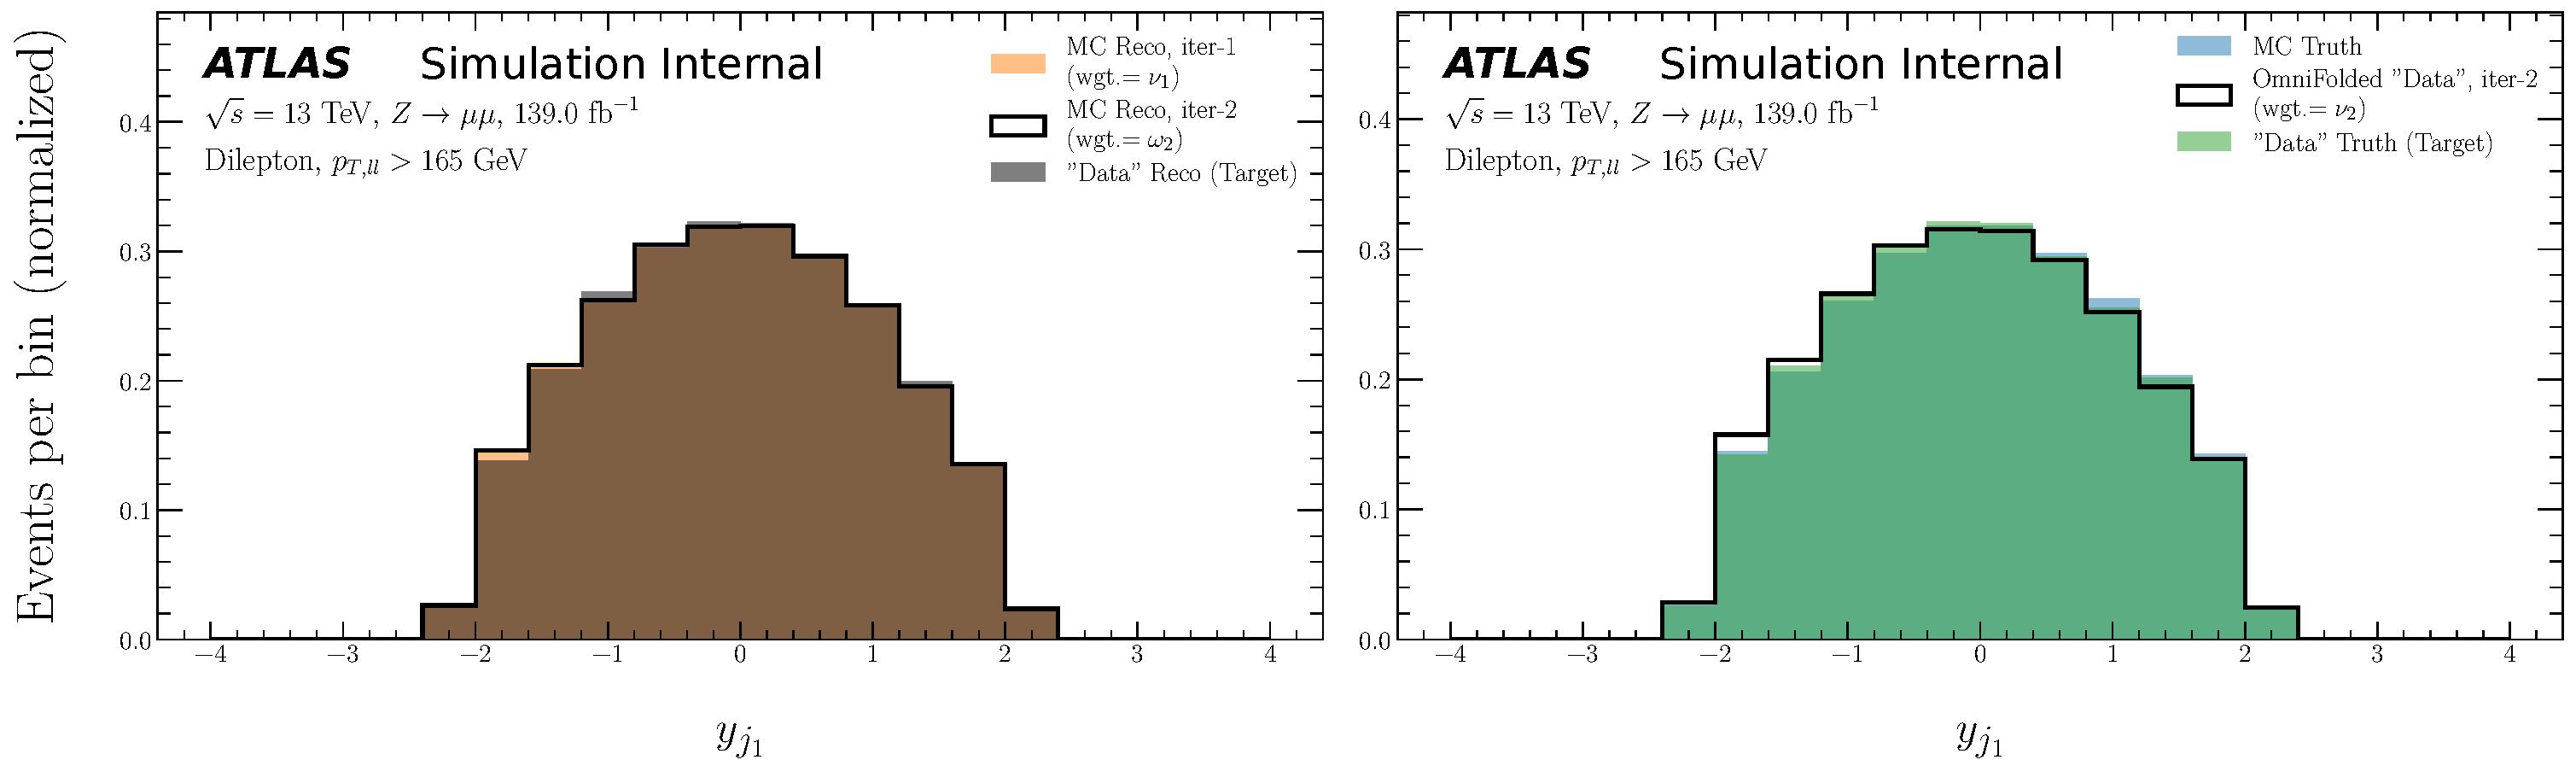
\includegraphics[width=0.85\textwidth]{figures/ATLASOmniFold-StressTest/ATLASOmniFold-StressTestC/MultiFold/y_trackj1/ATLASOmniFold-StressTestC-MultiFold-y_trackj1-Iteration02}}
\phantomcaption 
\end{figure}

\begin{figure}[h!]
\centering
\ContinuedFloat
\subfloat[After 3 iterations]{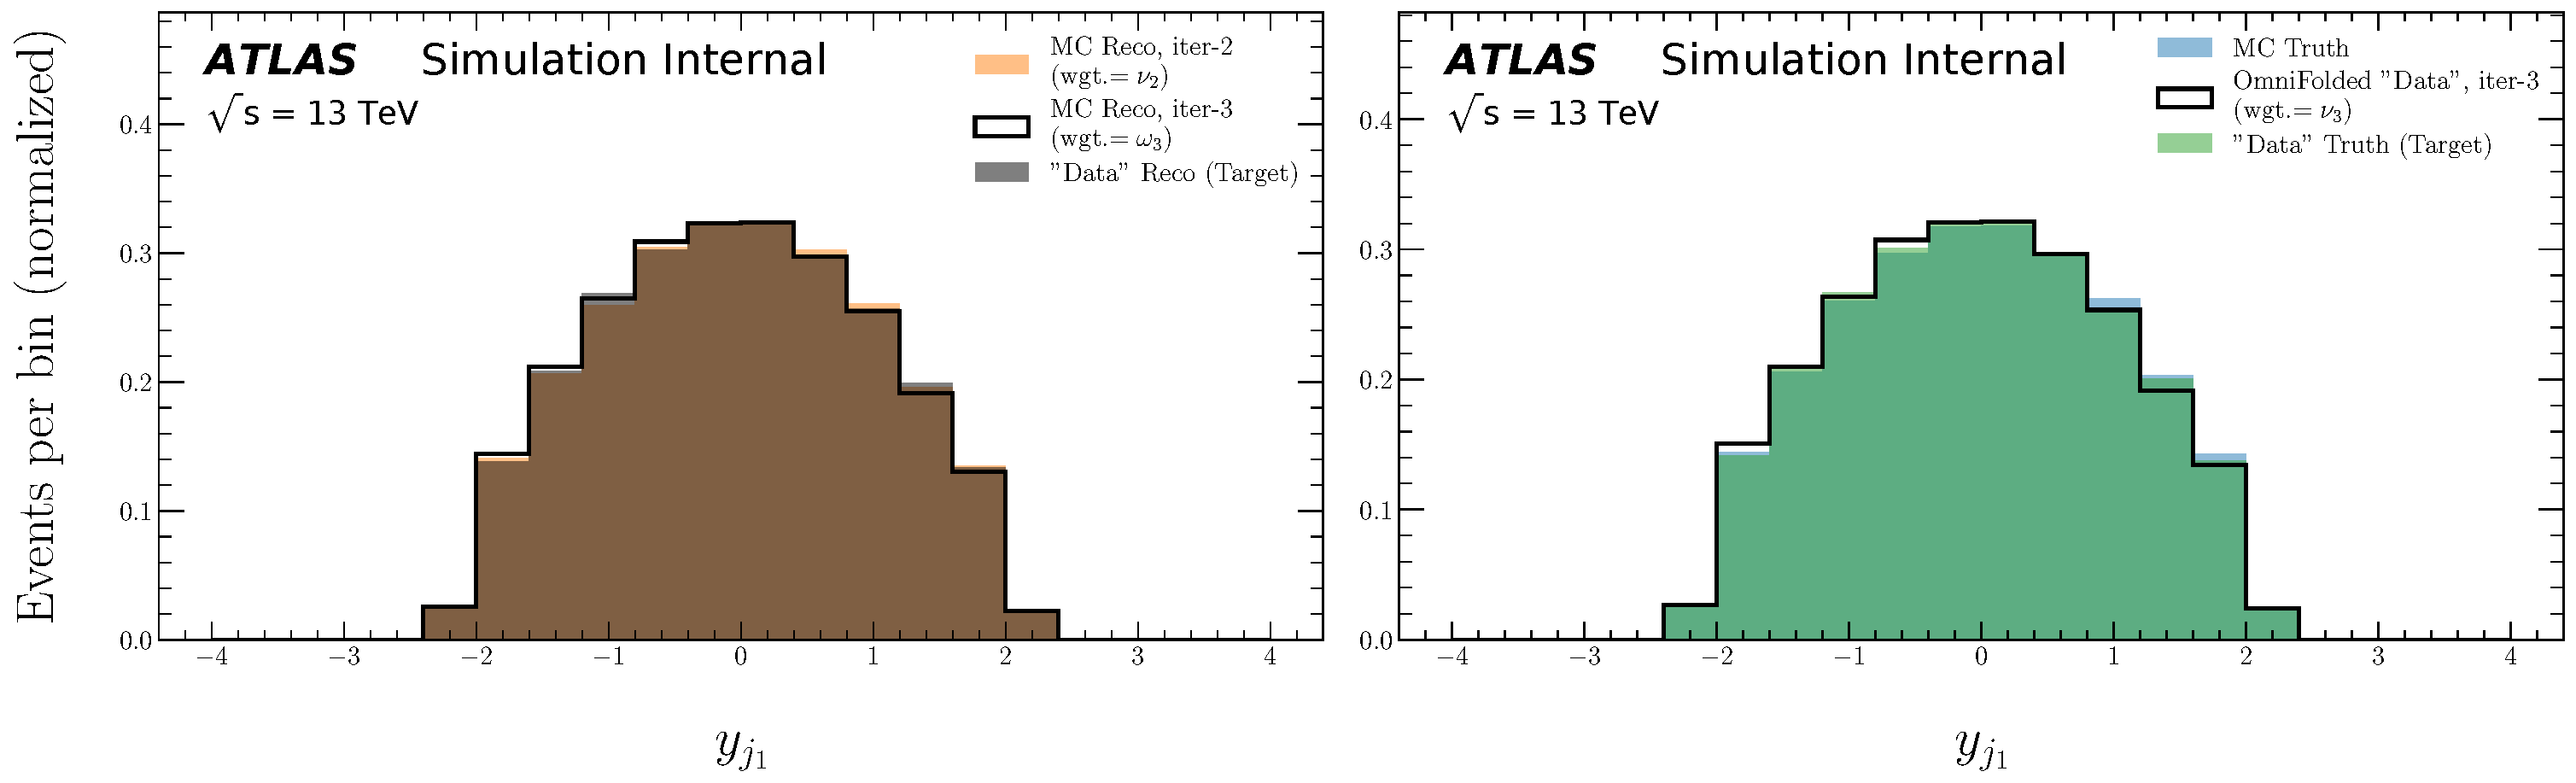
\includegraphics[width=0.85\textwidth]{figures/ATLASOmniFold-StressTest/ATLASOmniFold-StressTestC/MultiFold/y_trackj1/ATLASOmniFold-StressTestC-MultiFold-y_trackj1-Iteration03}}\\
\subfloat[After 4 iterations]{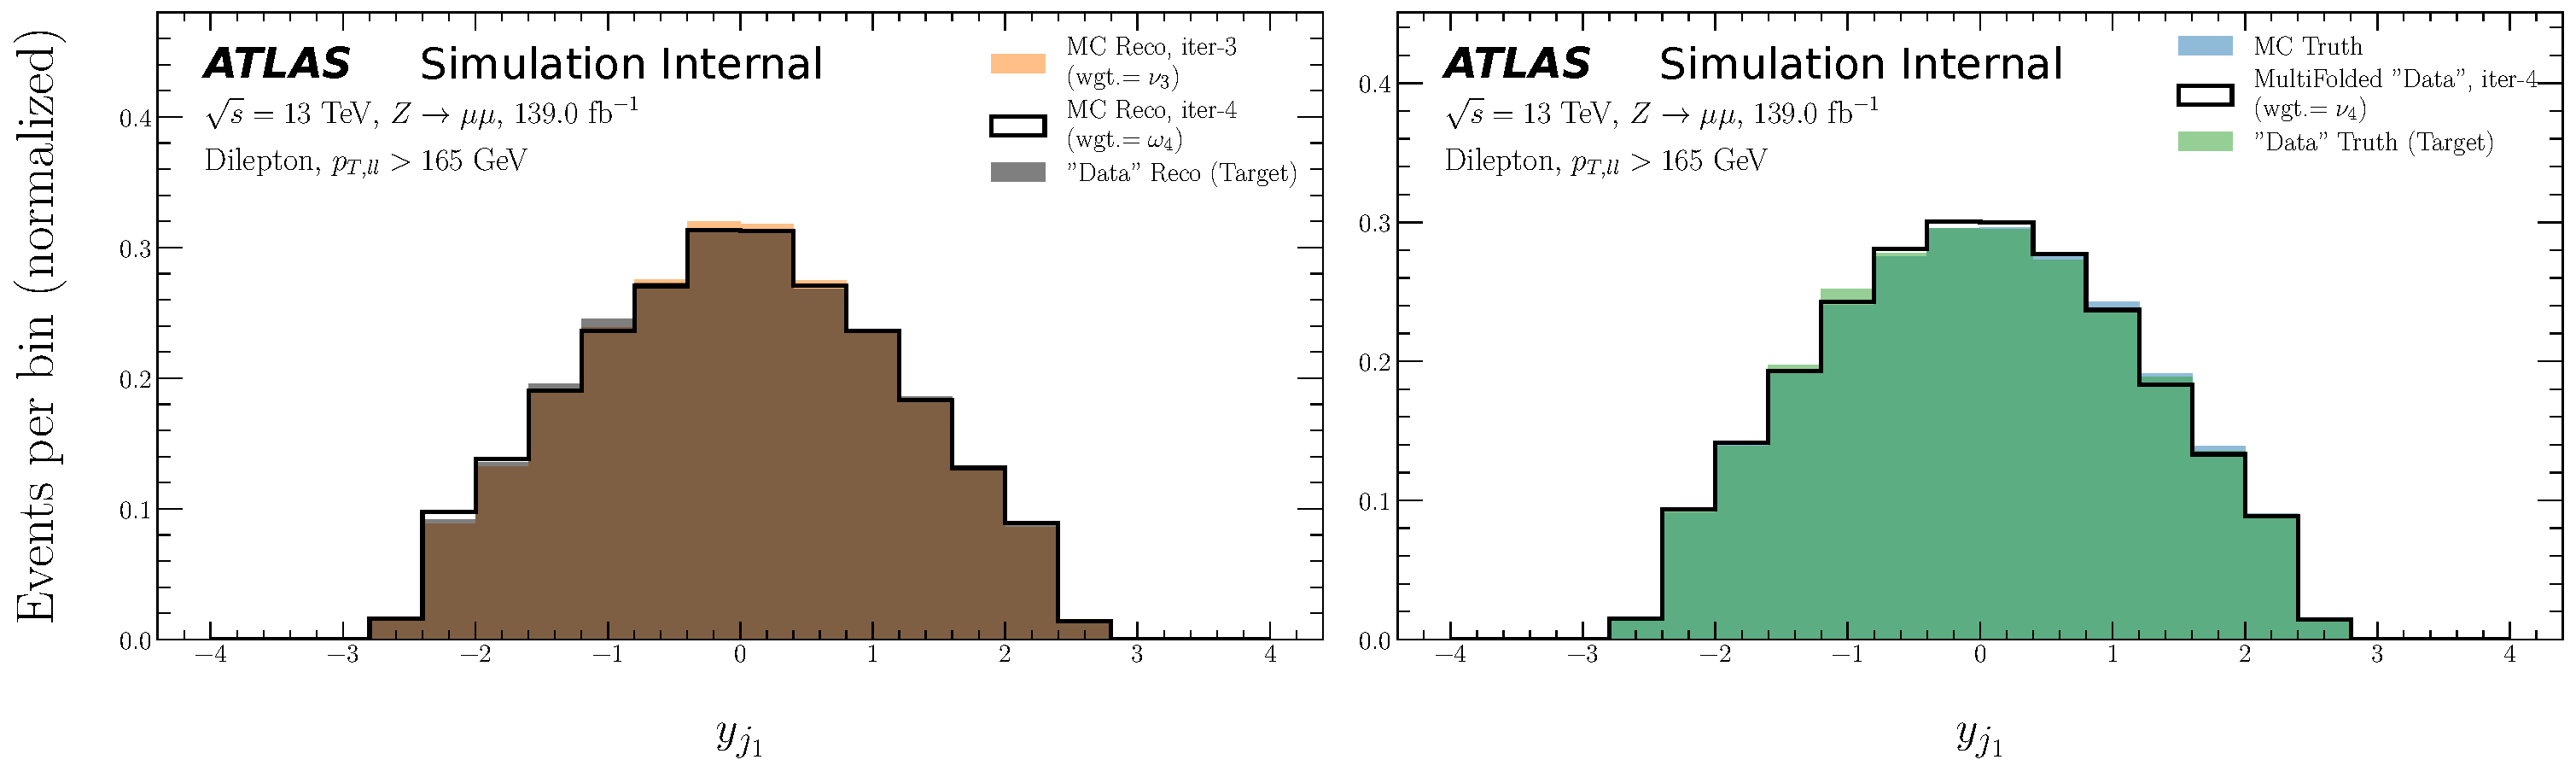
\includegraphics[width=0.85\textwidth]{figures/ATLASOmniFold-StressTest/ATLASOmniFold-StressTestC/MultiFold/y_trackj1/ATLASOmniFold-StressTestC-MultiFold-y_trackj1-Iteration04}}\\
\subfloat[After 5 iterations]{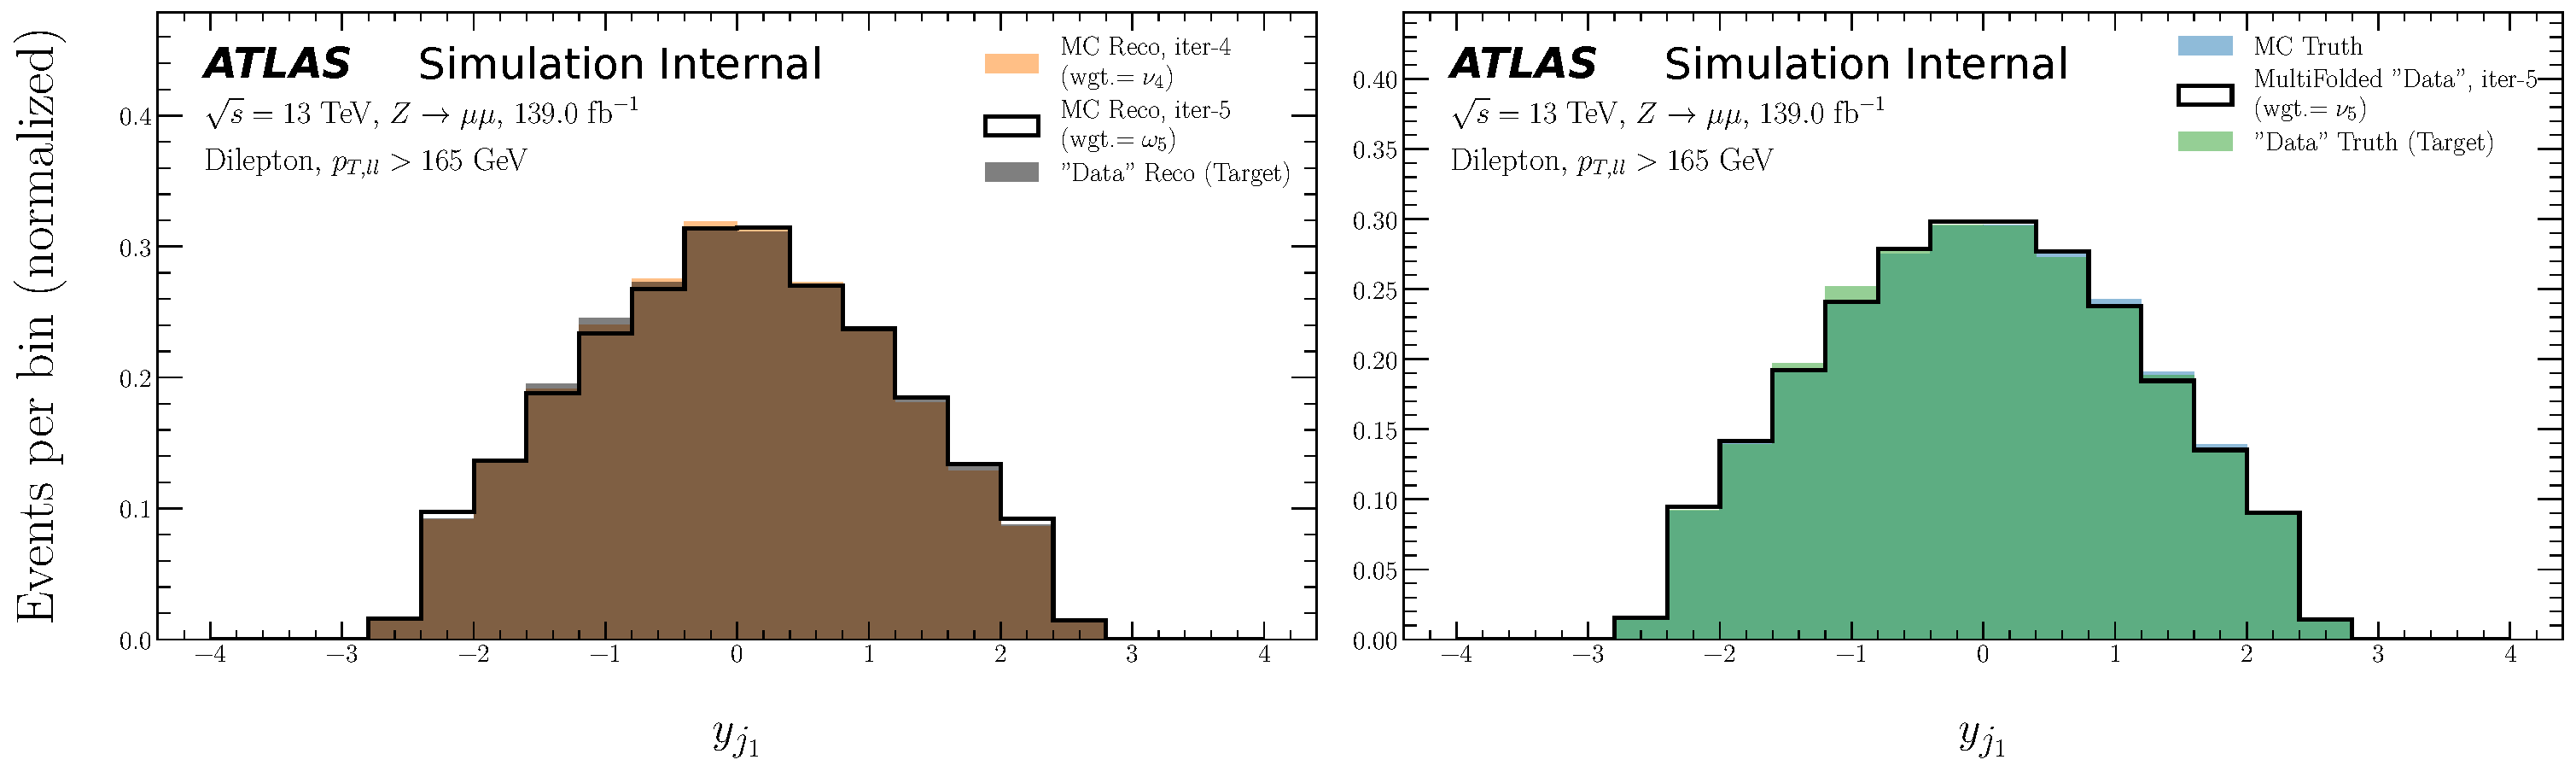
\includegraphics[width=0.85\textwidth]{figures/ATLASOmniFold-StressTest/ATLASOmniFold-StressTestC/MultiFold/y_trackj1/ATLASOmniFold-StressTestC-MultiFold-y_trackj1-Iteration05}}\\
\subfloat[After 6 iterations]{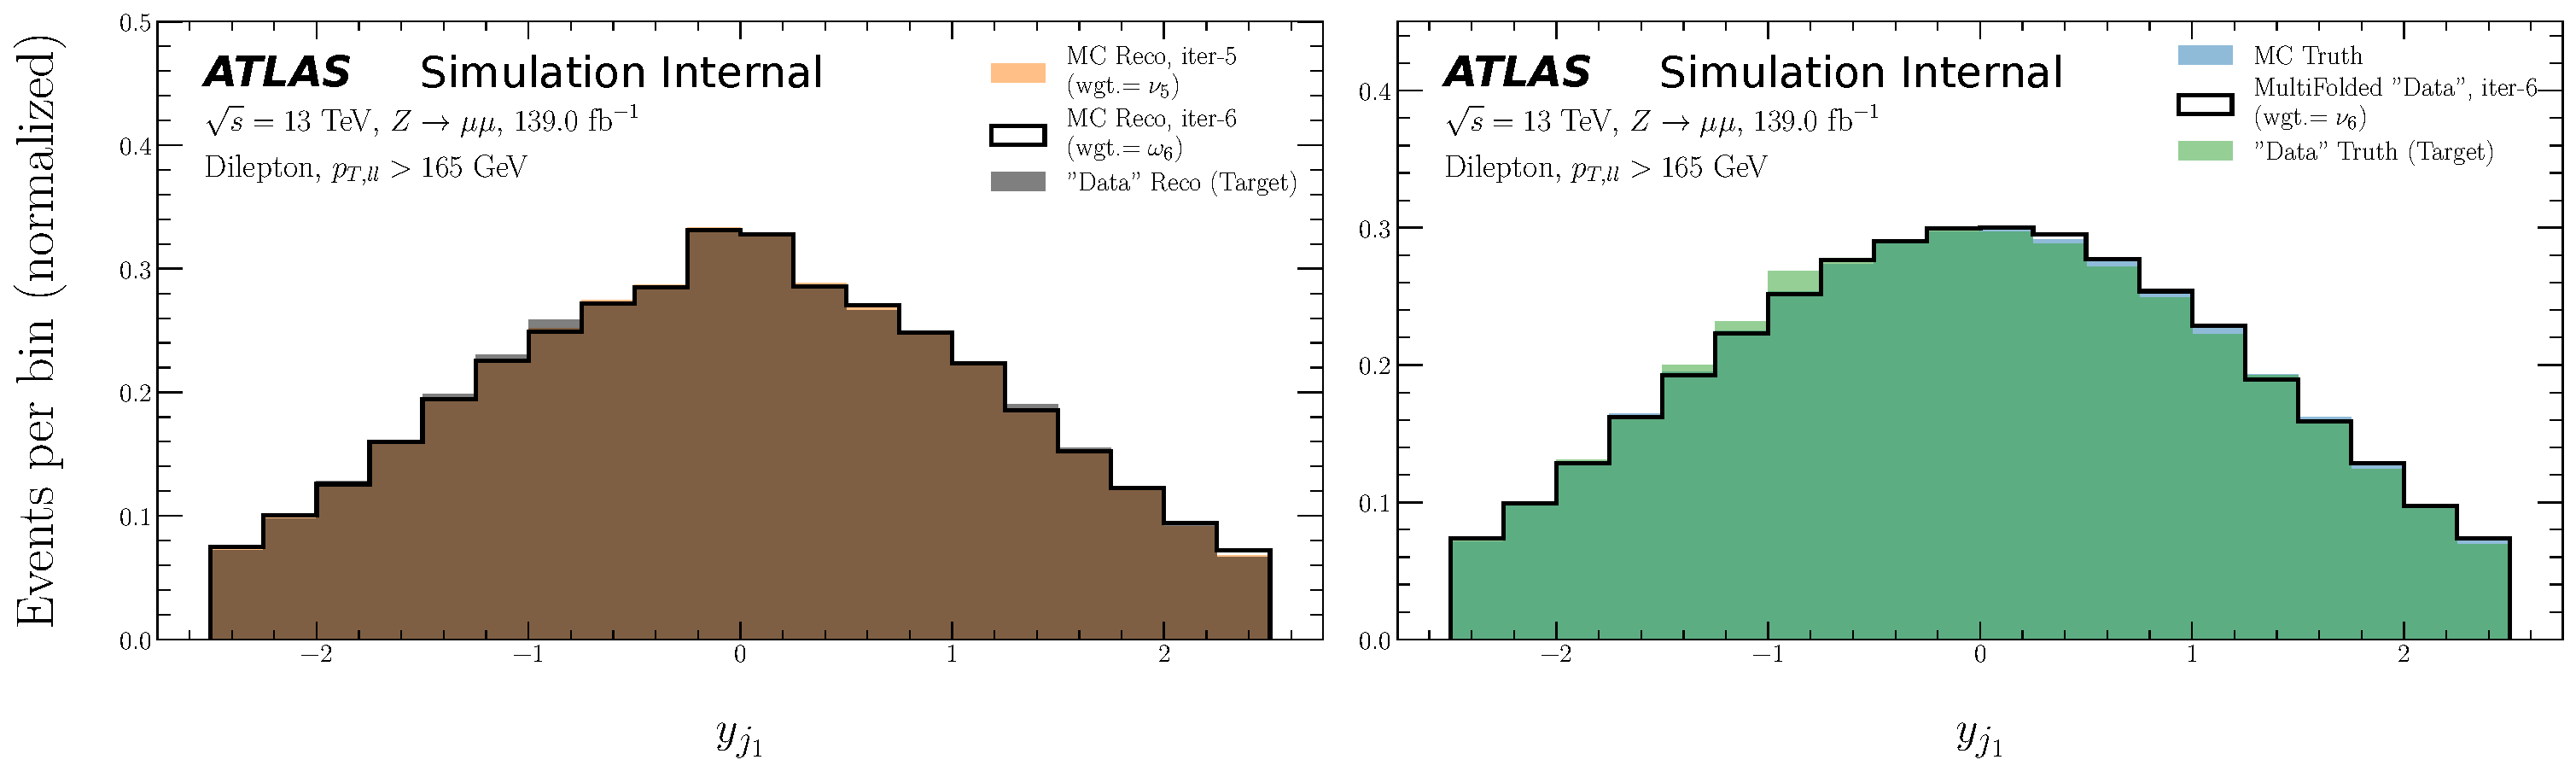
\includegraphics[width=0.85\textwidth]{figures/ATLASOmniFold-StressTest/ATLASOmniFold-StressTestC/MultiFold/y_trackj1/ATLASOmniFold-StressTestC-MultiFold-y_trackj1-Iteration06}}
\caption{MultiFolding Sherpa with Pythia for the leading track jet rapidity.}
\label{fig:stressc_y_trackj1Multi}
\end{figure}

\begin{figure}[h!]
\centering
\subfloat[Input histograms]{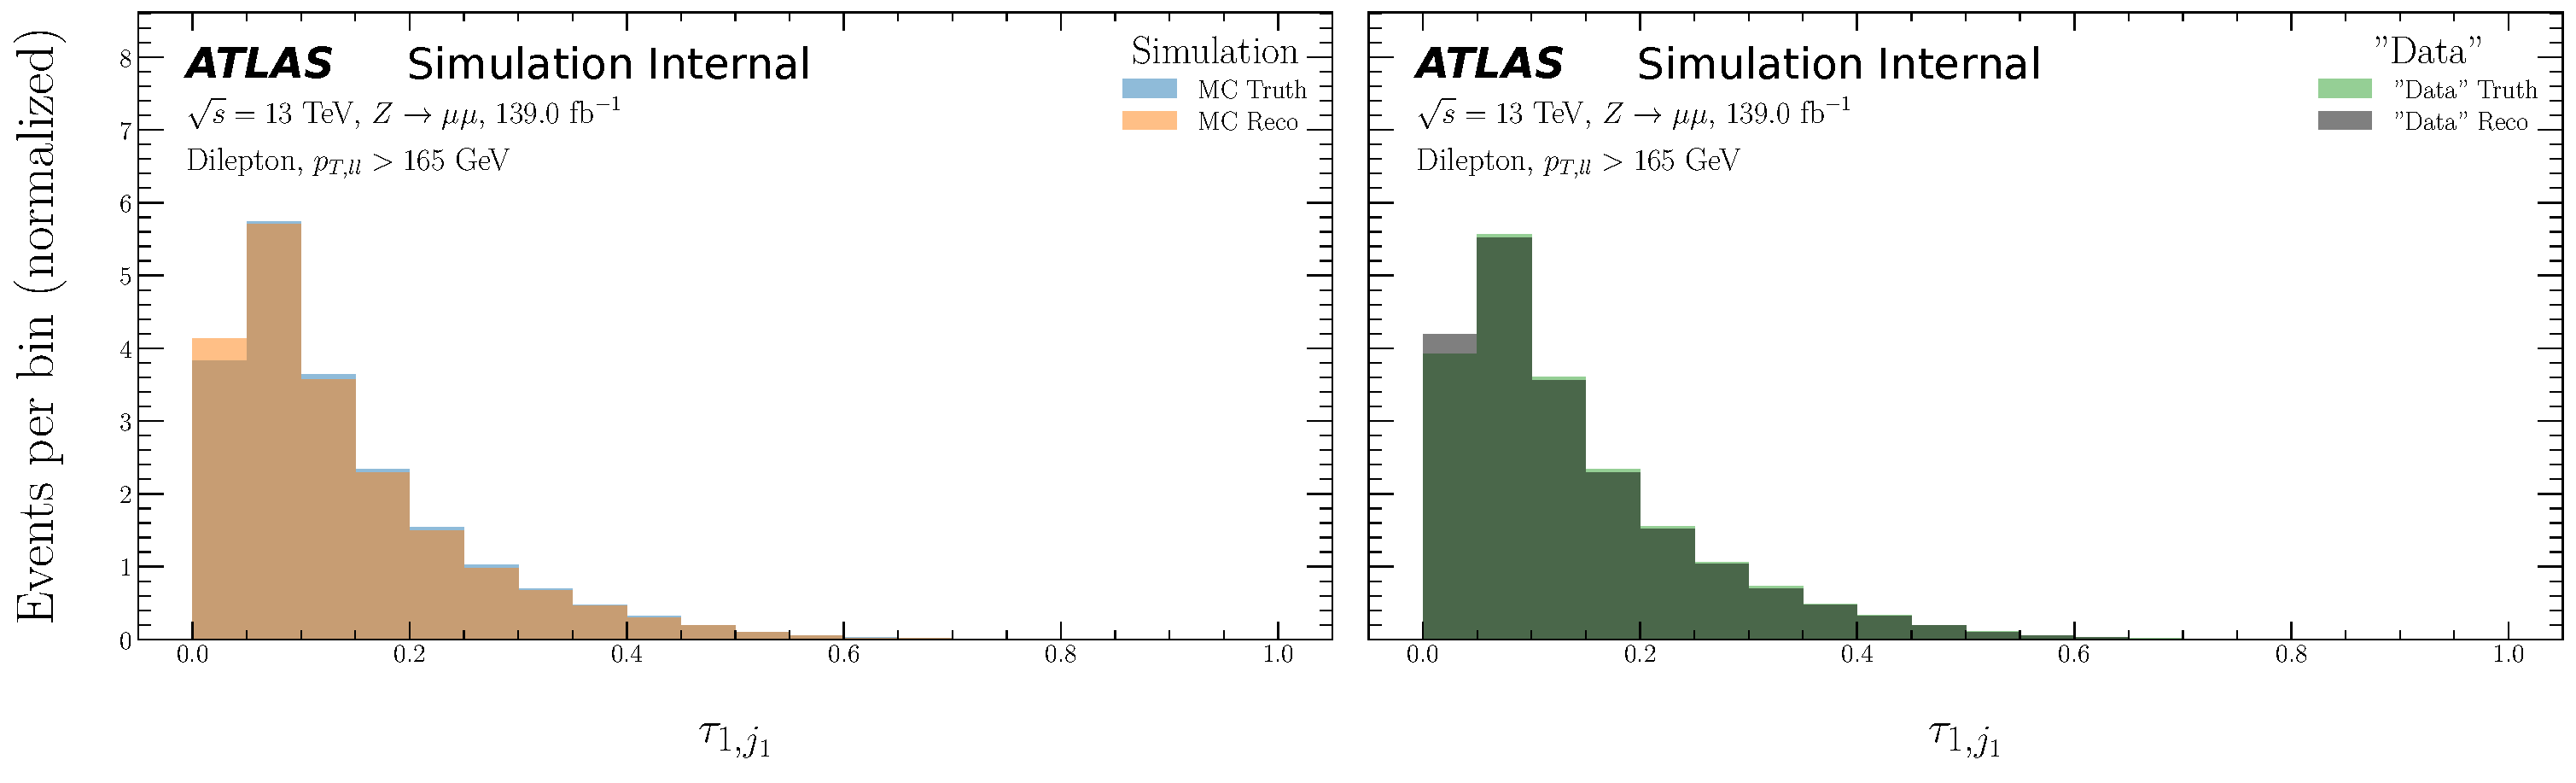
\includegraphics[width=0.85\textwidth]{figures/ATLASOmniFold-StressTest/ATLASOmniFold-StressTestC/MultiFold/tau1_trackj1/ATLASOmniFold-StressTestC-MultiFold-tau1_trackj1-Distributions}}\\
\subfloat[After 1 iteration]{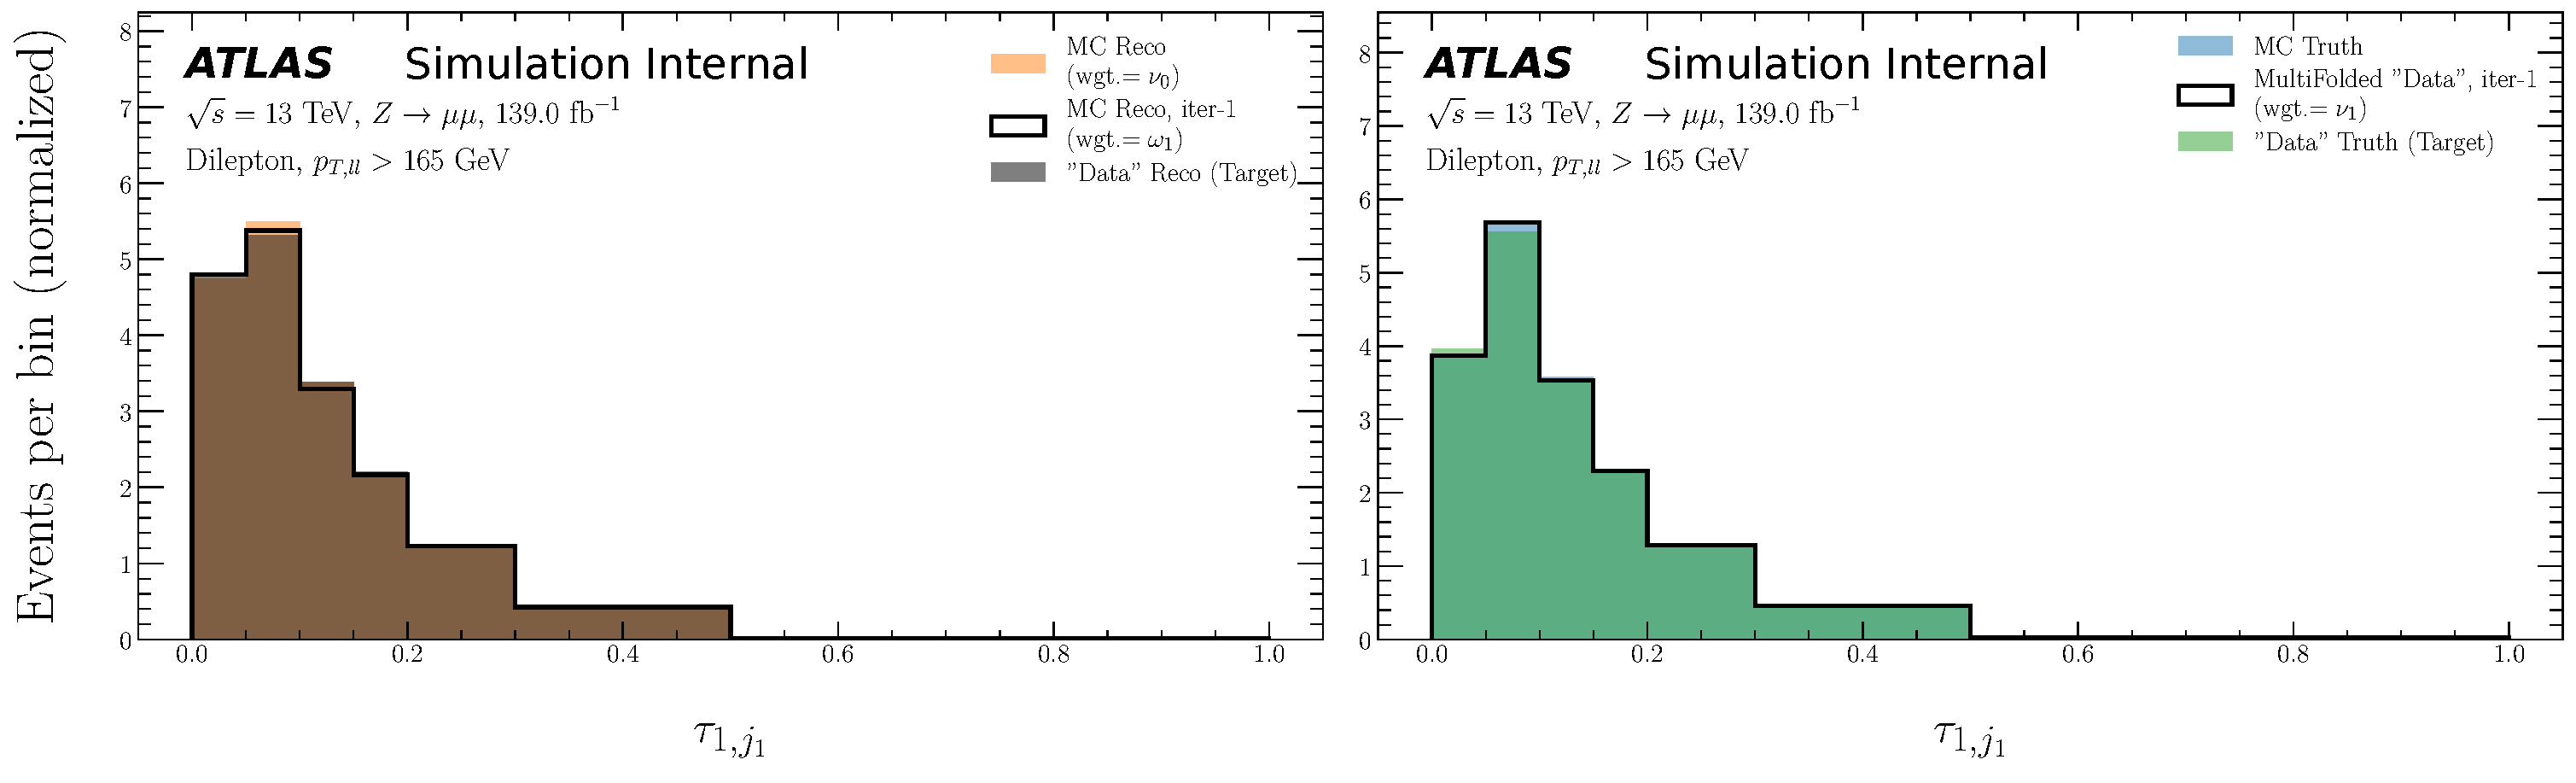
\includegraphics[width=0.85\textwidth]{figures/ATLASOmniFold-StressTest/ATLASOmniFold-StressTestC/MultiFold/tau1_trackj1/ATLASOmniFold-StressTestC-MultiFold-tau1_trackj1-Iteration01}}\\
\subfloat[After 2 iterations]{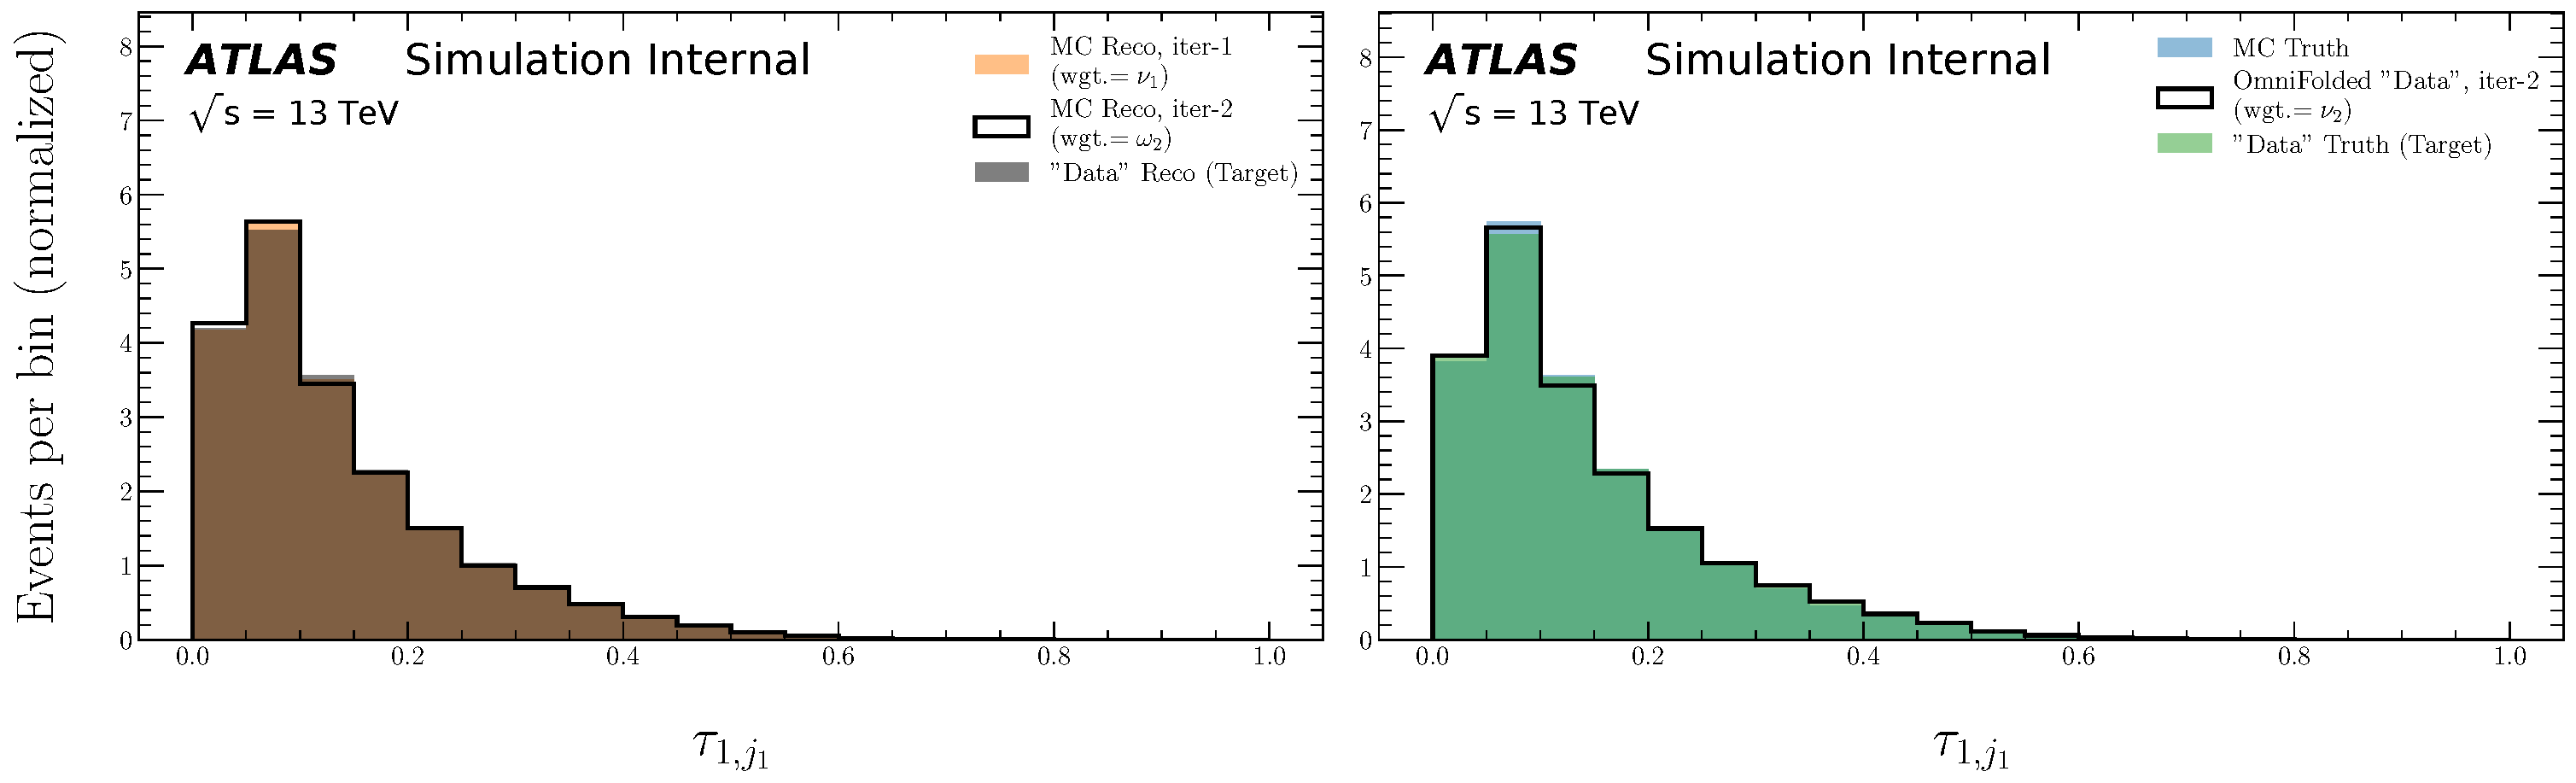
\includegraphics[width=0.85\textwidth]{figures/ATLASOmniFold-StressTest/ATLASOmniFold-StressTestC/MultiFold/tau1_trackj1/ATLASOmniFold-StressTestC-MultiFold-tau1_trackj1-Iteration02}}
\phantomcaption 
\end{figure}

\begin{figure}[h!]
\centering
\ContinuedFloat
\subfloat[After 3 iterations]{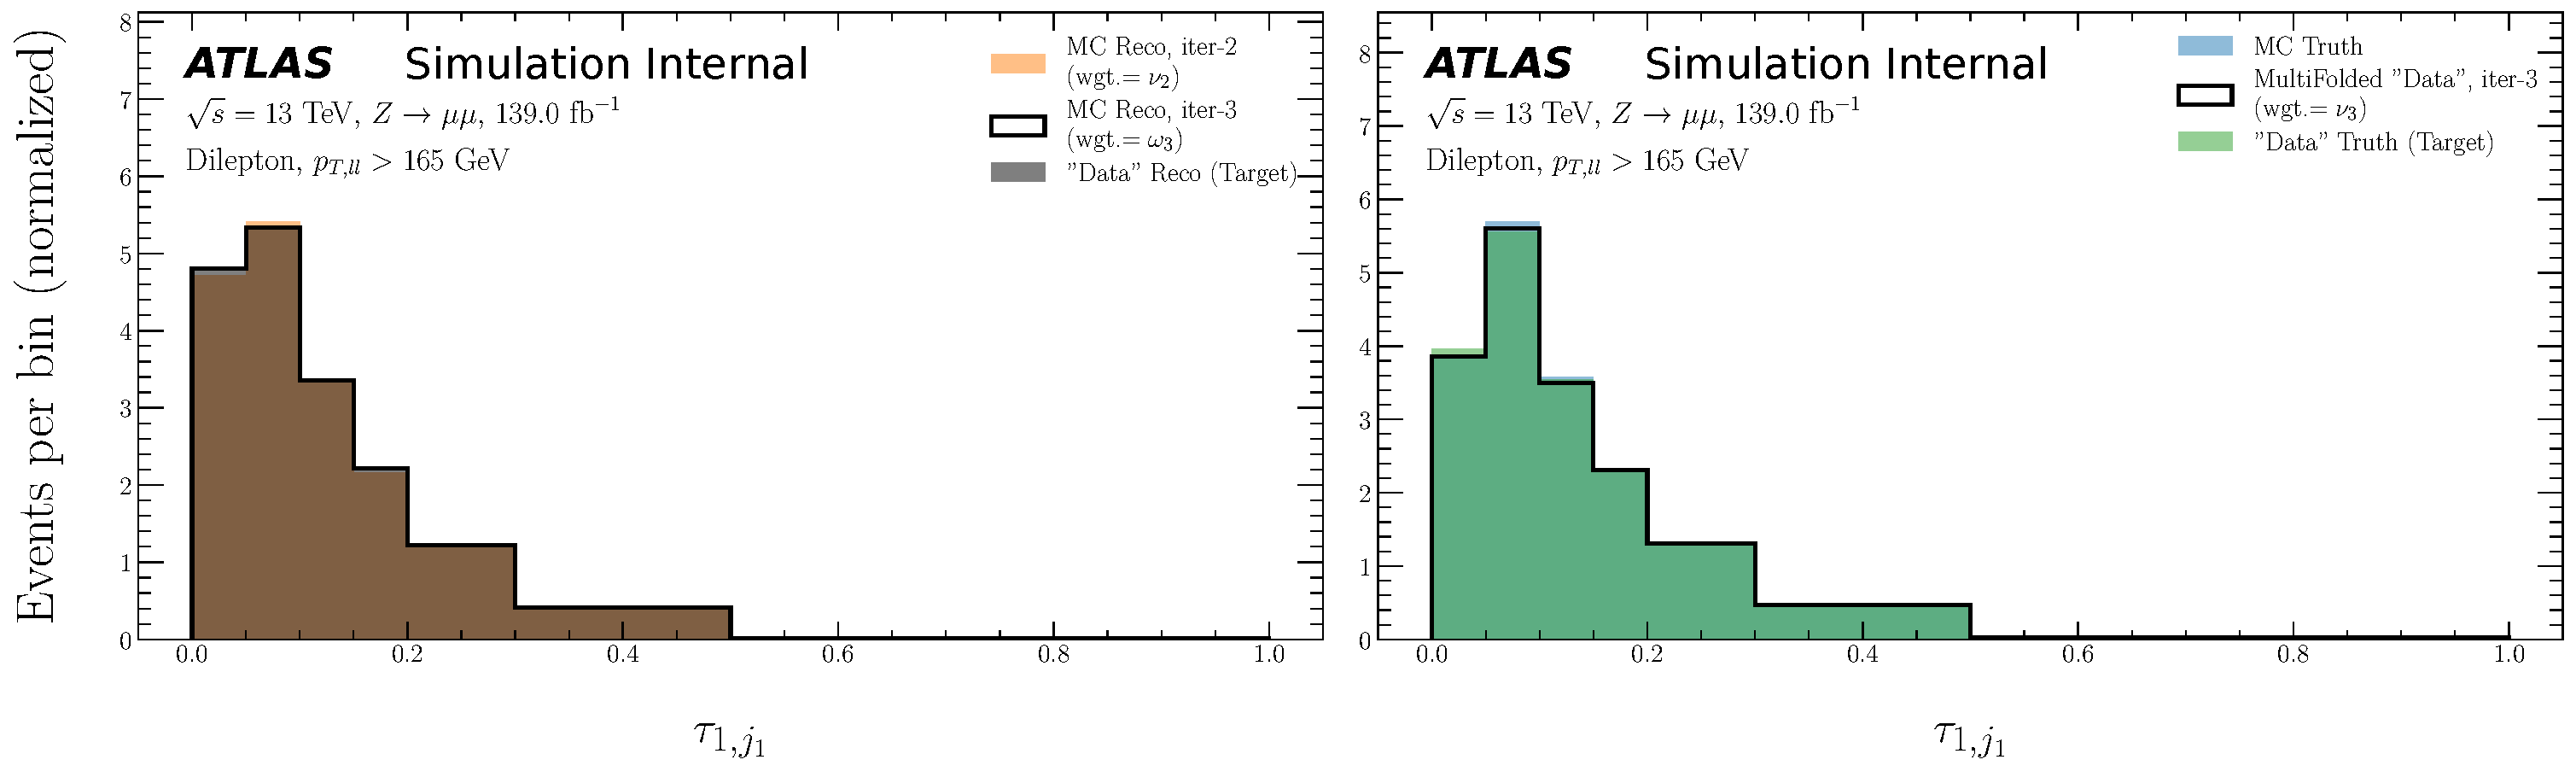
\includegraphics[width=0.85\textwidth]{figures/ATLASOmniFold-StressTest/ATLASOmniFold-StressTestC/MultiFold/tau1_trackj1/ATLASOmniFold-StressTestC-MultiFold-tau1_trackj1-Iteration03}}\\
\subfloat[After 4 iterations]{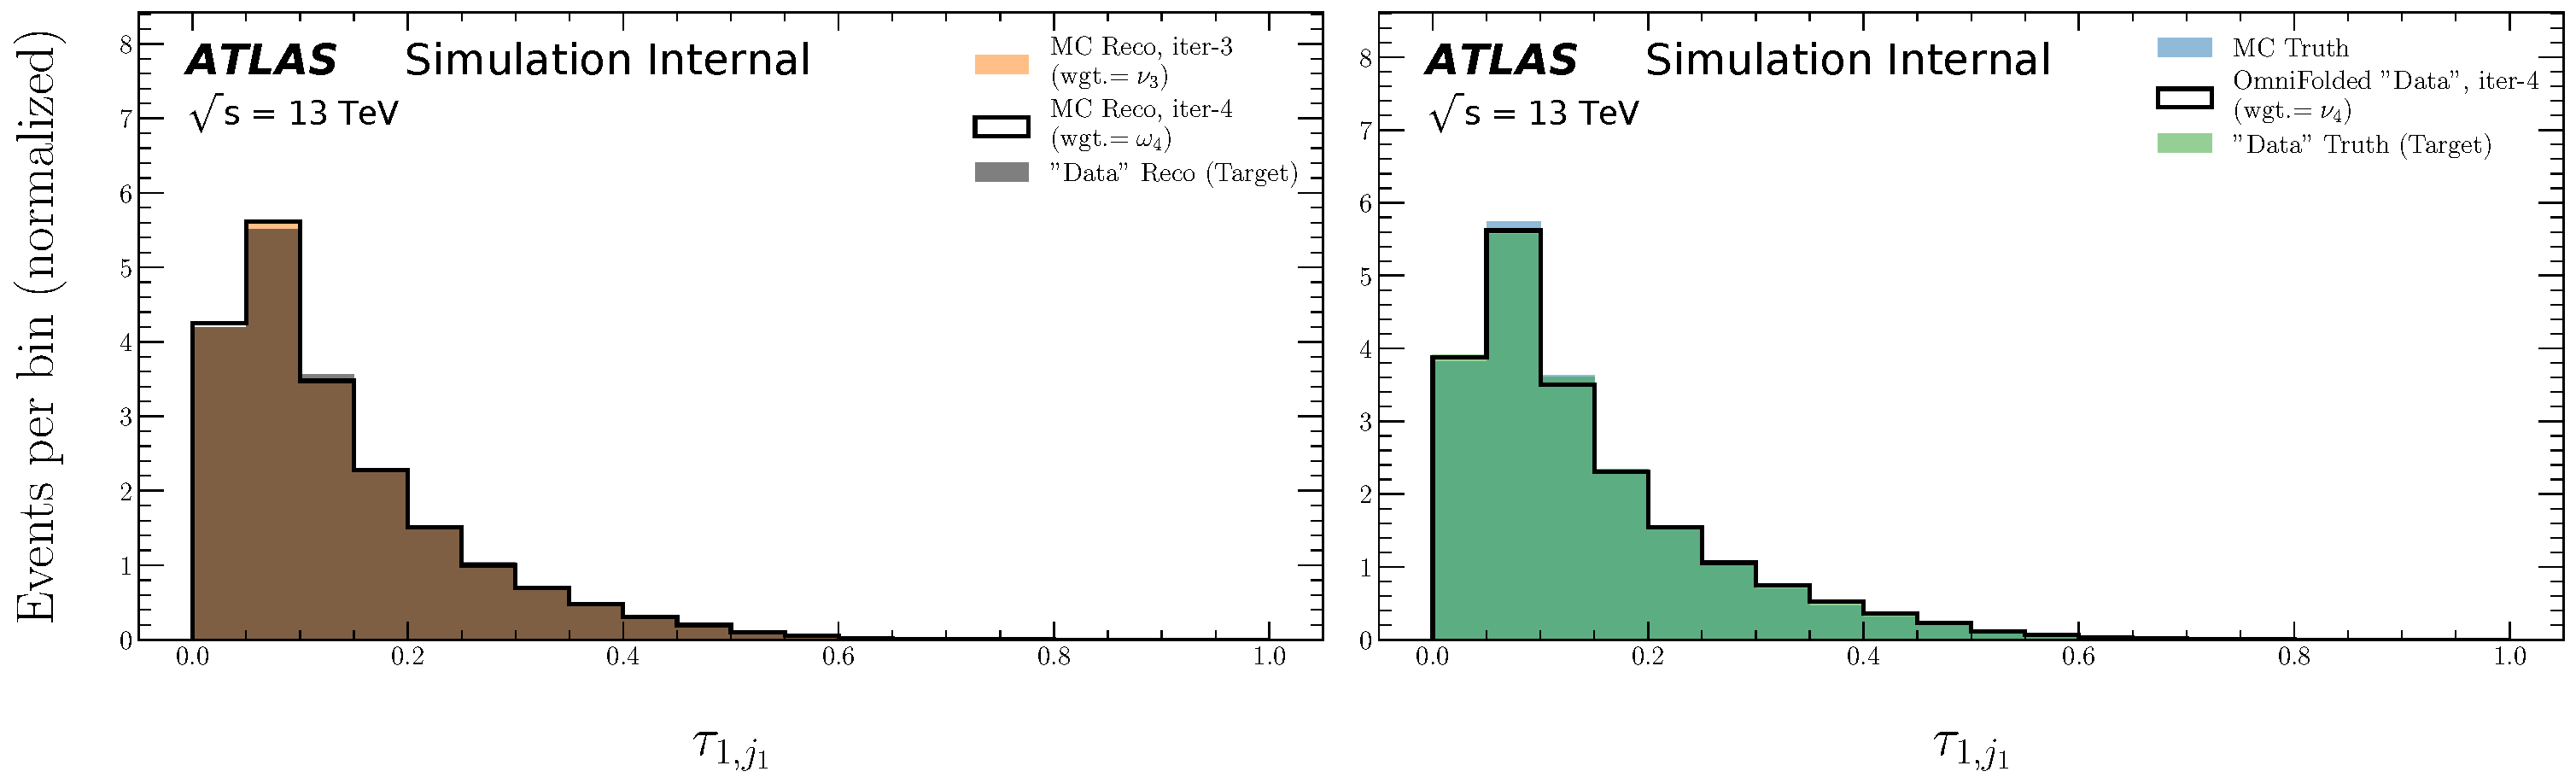
\includegraphics[width=0.85\textwidth]{figures/ATLASOmniFold-StressTest/ATLASOmniFold-StressTestC/MultiFold/tau1_trackj1/ATLASOmniFold-StressTestC-MultiFold-tau1_trackj1-Iteration04}}\\
\subfloat[After 5 iterations]{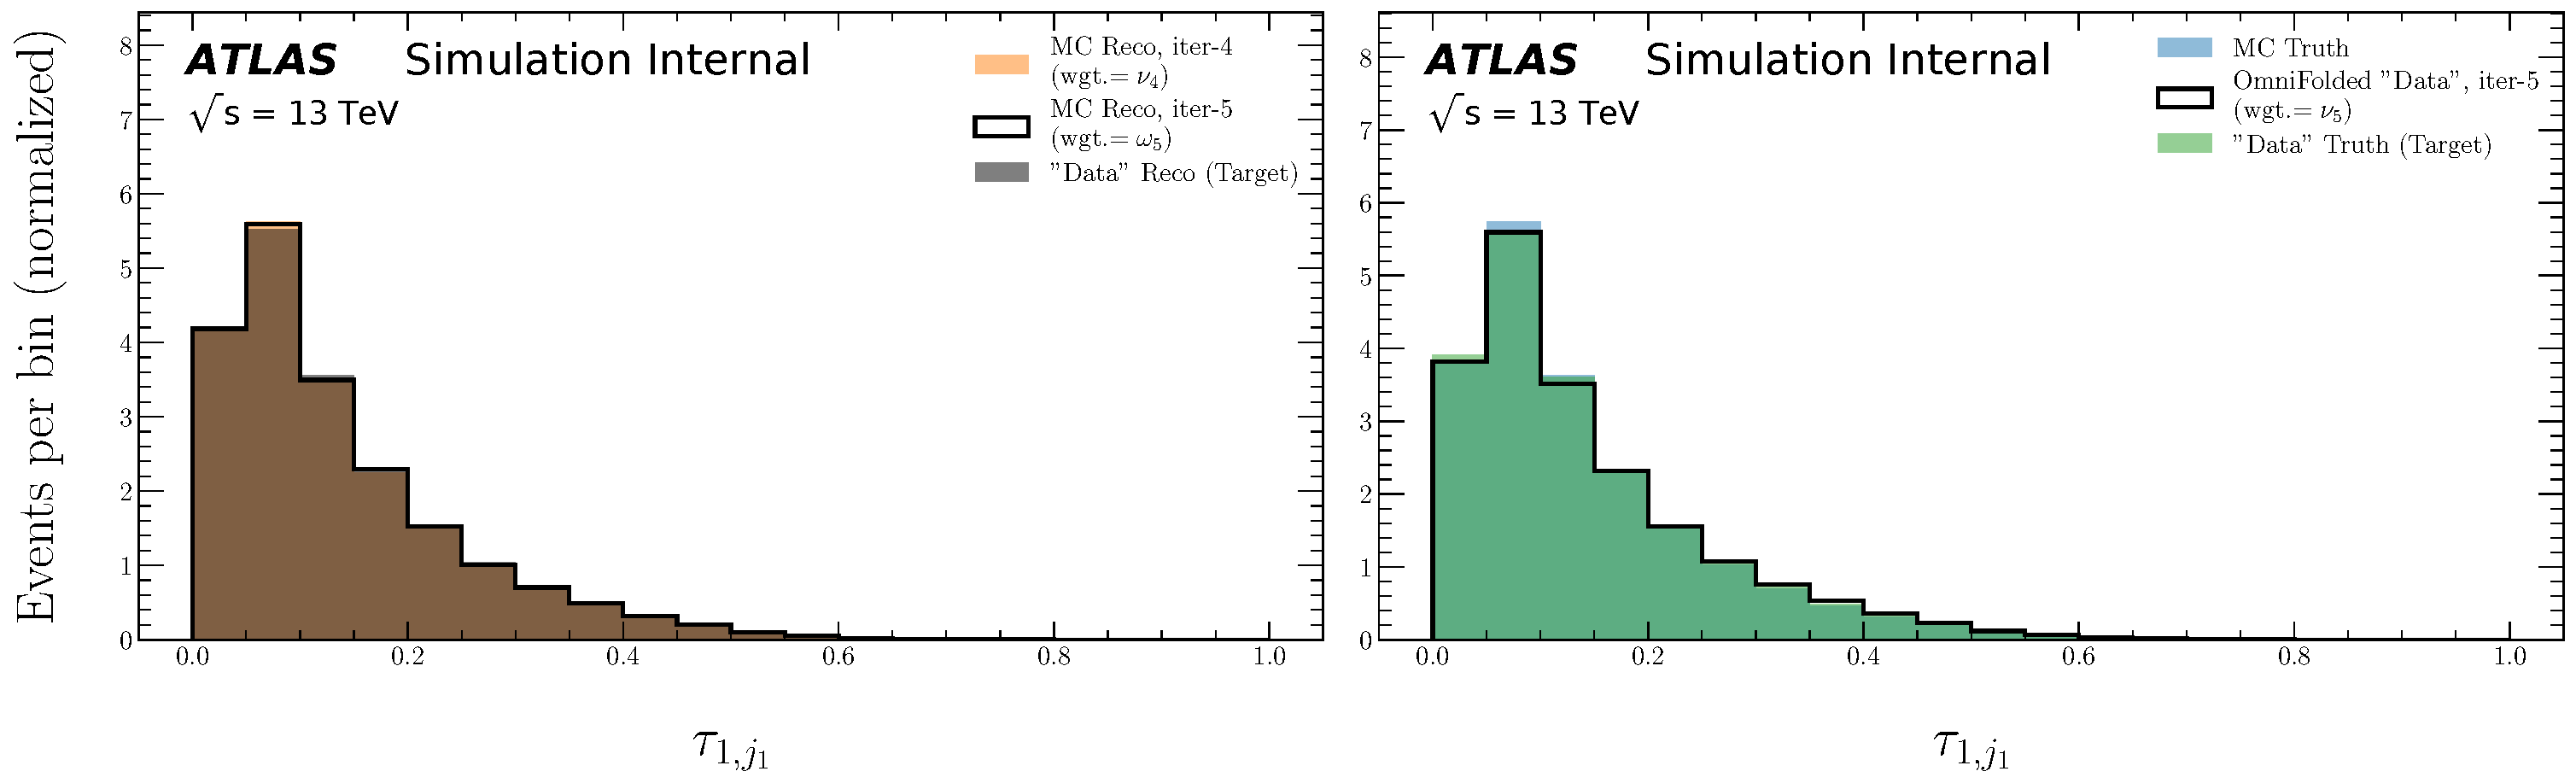
\includegraphics[width=0.85\textwidth]{figures/ATLASOmniFold-StressTest/ATLASOmniFold-StressTestC/MultiFold/tau1_trackj1/ATLASOmniFold-StressTestC-MultiFold-tau1_trackj1-Iteration05}}\\
\subfloat[After 6 iterations]{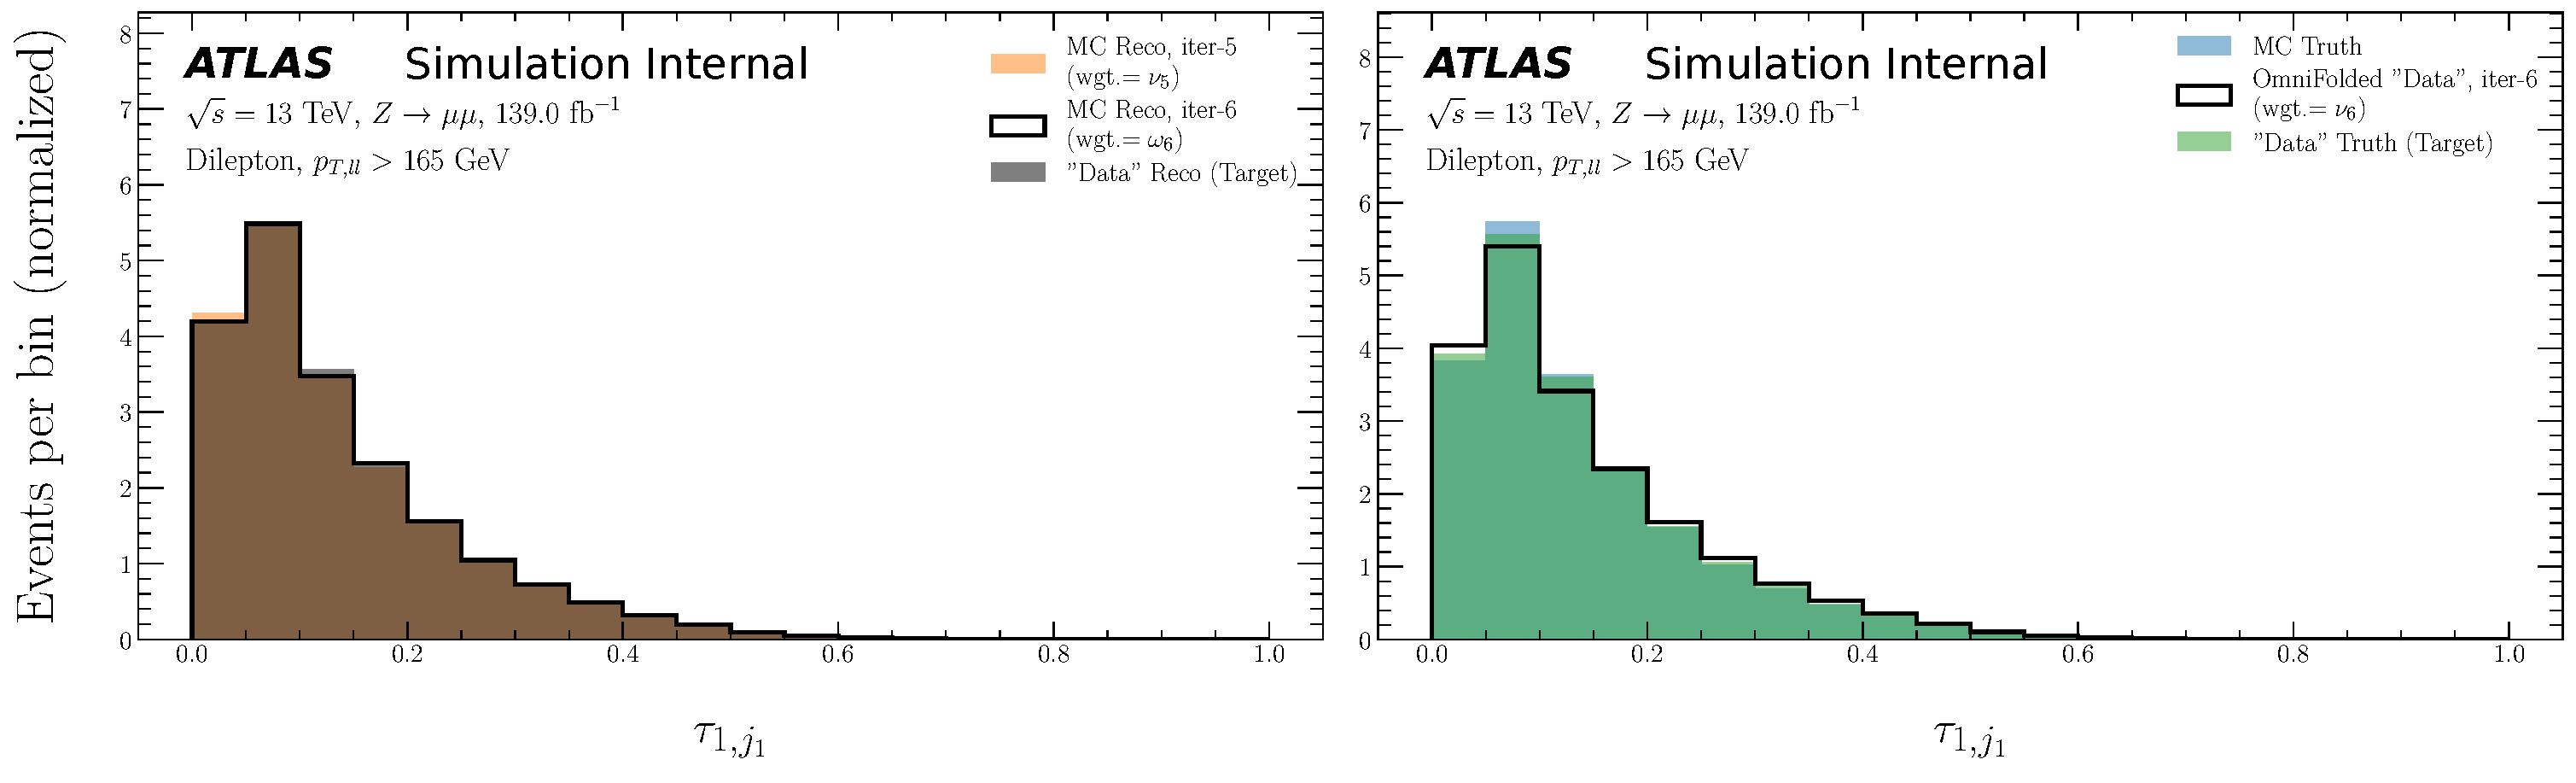
\includegraphics[width=0.85\textwidth]{figures/ATLASOmniFold-StressTest/ATLASOmniFold-StressTestC/MultiFold/tau1_trackj1/ATLASOmniFold-StressTestC-MultiFold-tau1_trackj1-Iteration06}}
\caption{MultiFolding Sherpa with Pythia for the leading track jet $\tau_1$.}
\label{fig:stressc_tau1_trackj1Multi}
\end{figure}

\begin{figure}[h!]
\centering
\subfloat[Input histograms]{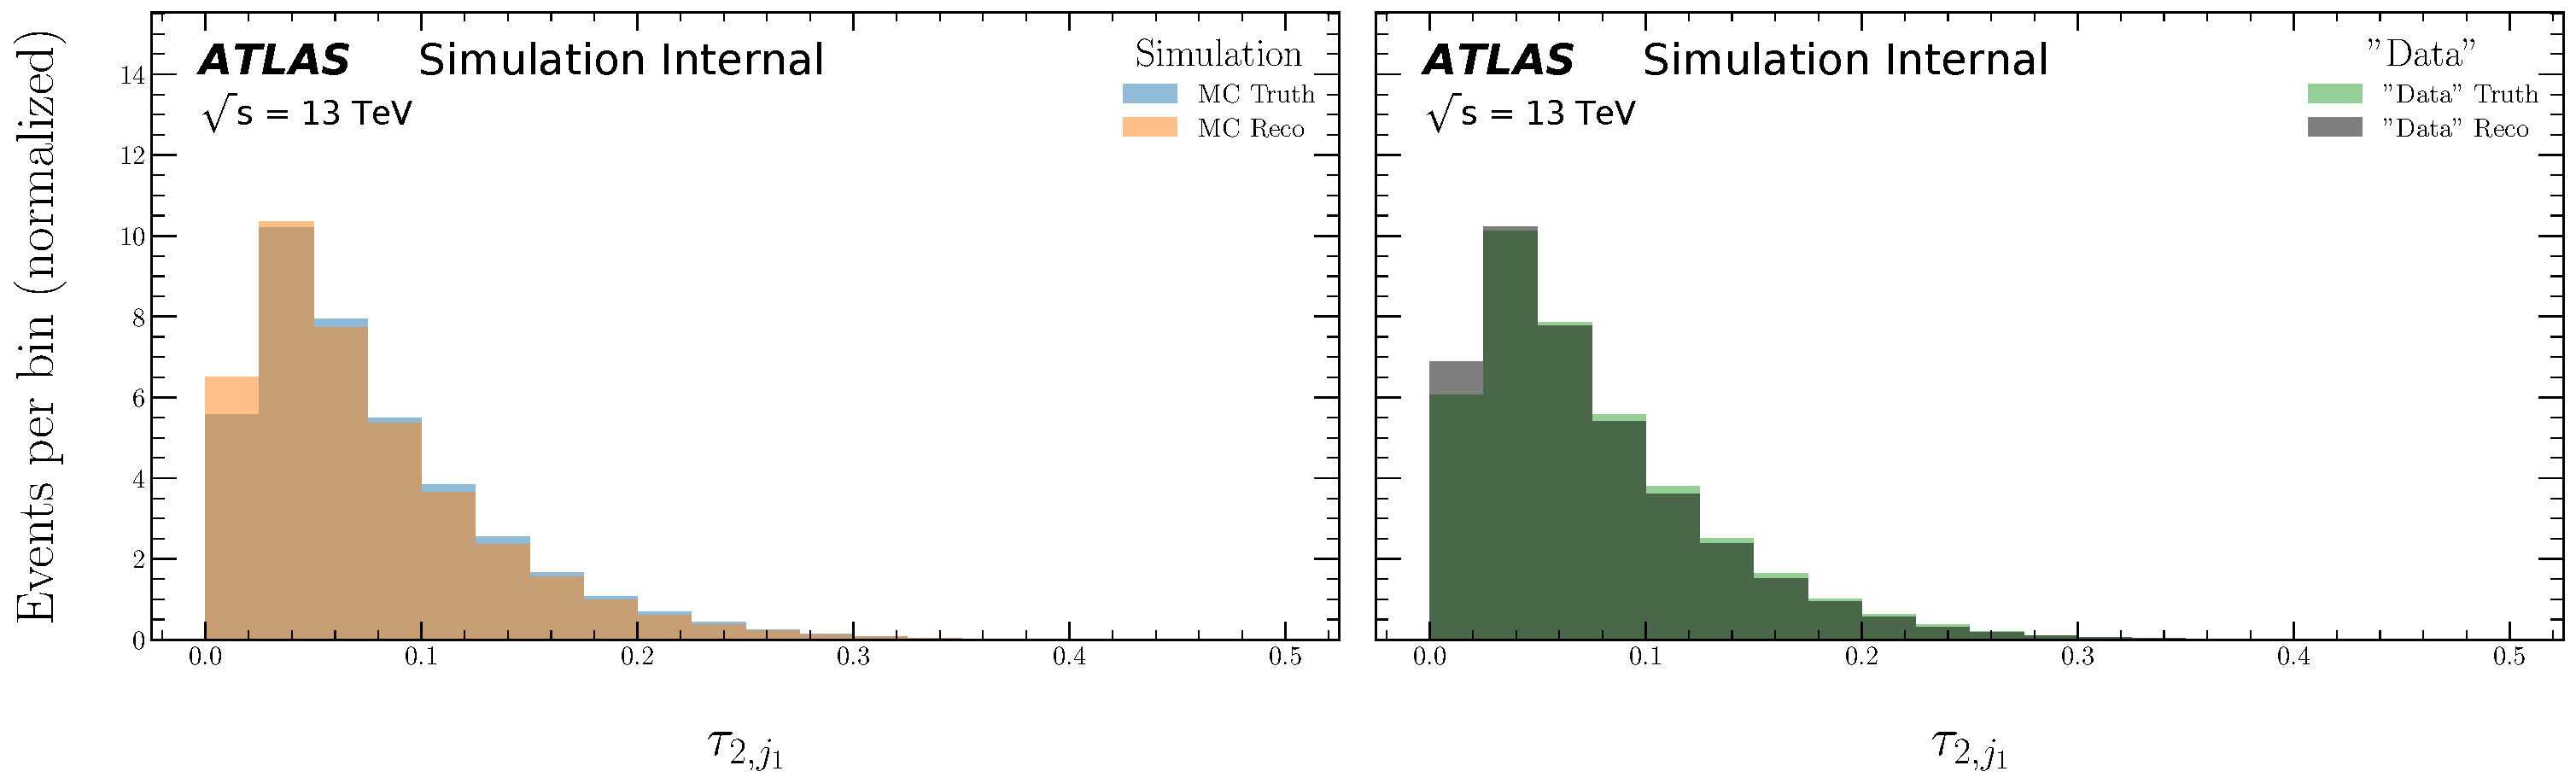
\includegraphics[width=0.85\textwidth]{figures/ATLASOmniFold-StressTest/ATLASOmniFold-StressTestC/MultiFold/tau2_trackj1/ATLASOmniFold-StressTestC-MultiFold-tau2_trackj1-Distributions}}\\
\subfloat[After 1 iteration]{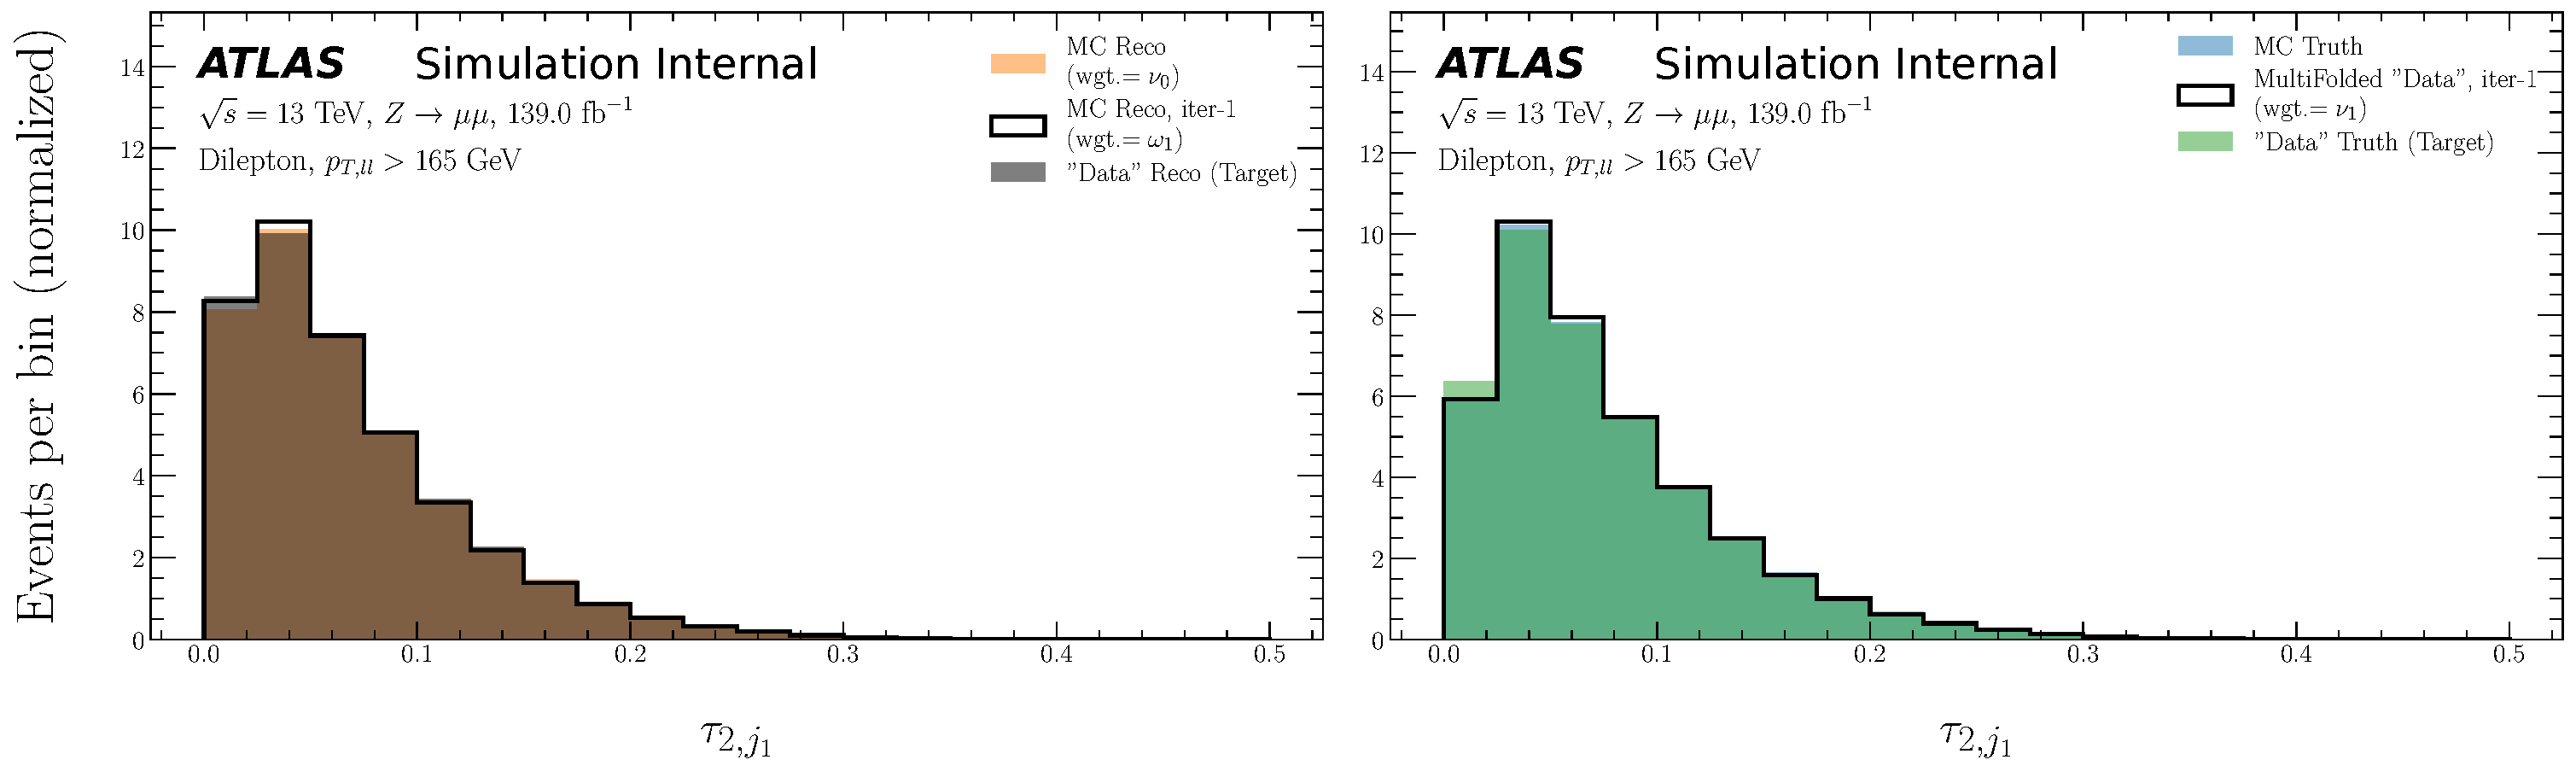
\includegraphics[width=0.85\textwidth]{figures/ATLASOmniFold-StressTest/ATLASOmniFold-StressTestC/MultiFold/tau2_trackj1/ATLASOmniFold-StressTestC-MultiFold-tau2_trackj1-Iteration01}}\\
\subfloat[After 2 iterations]{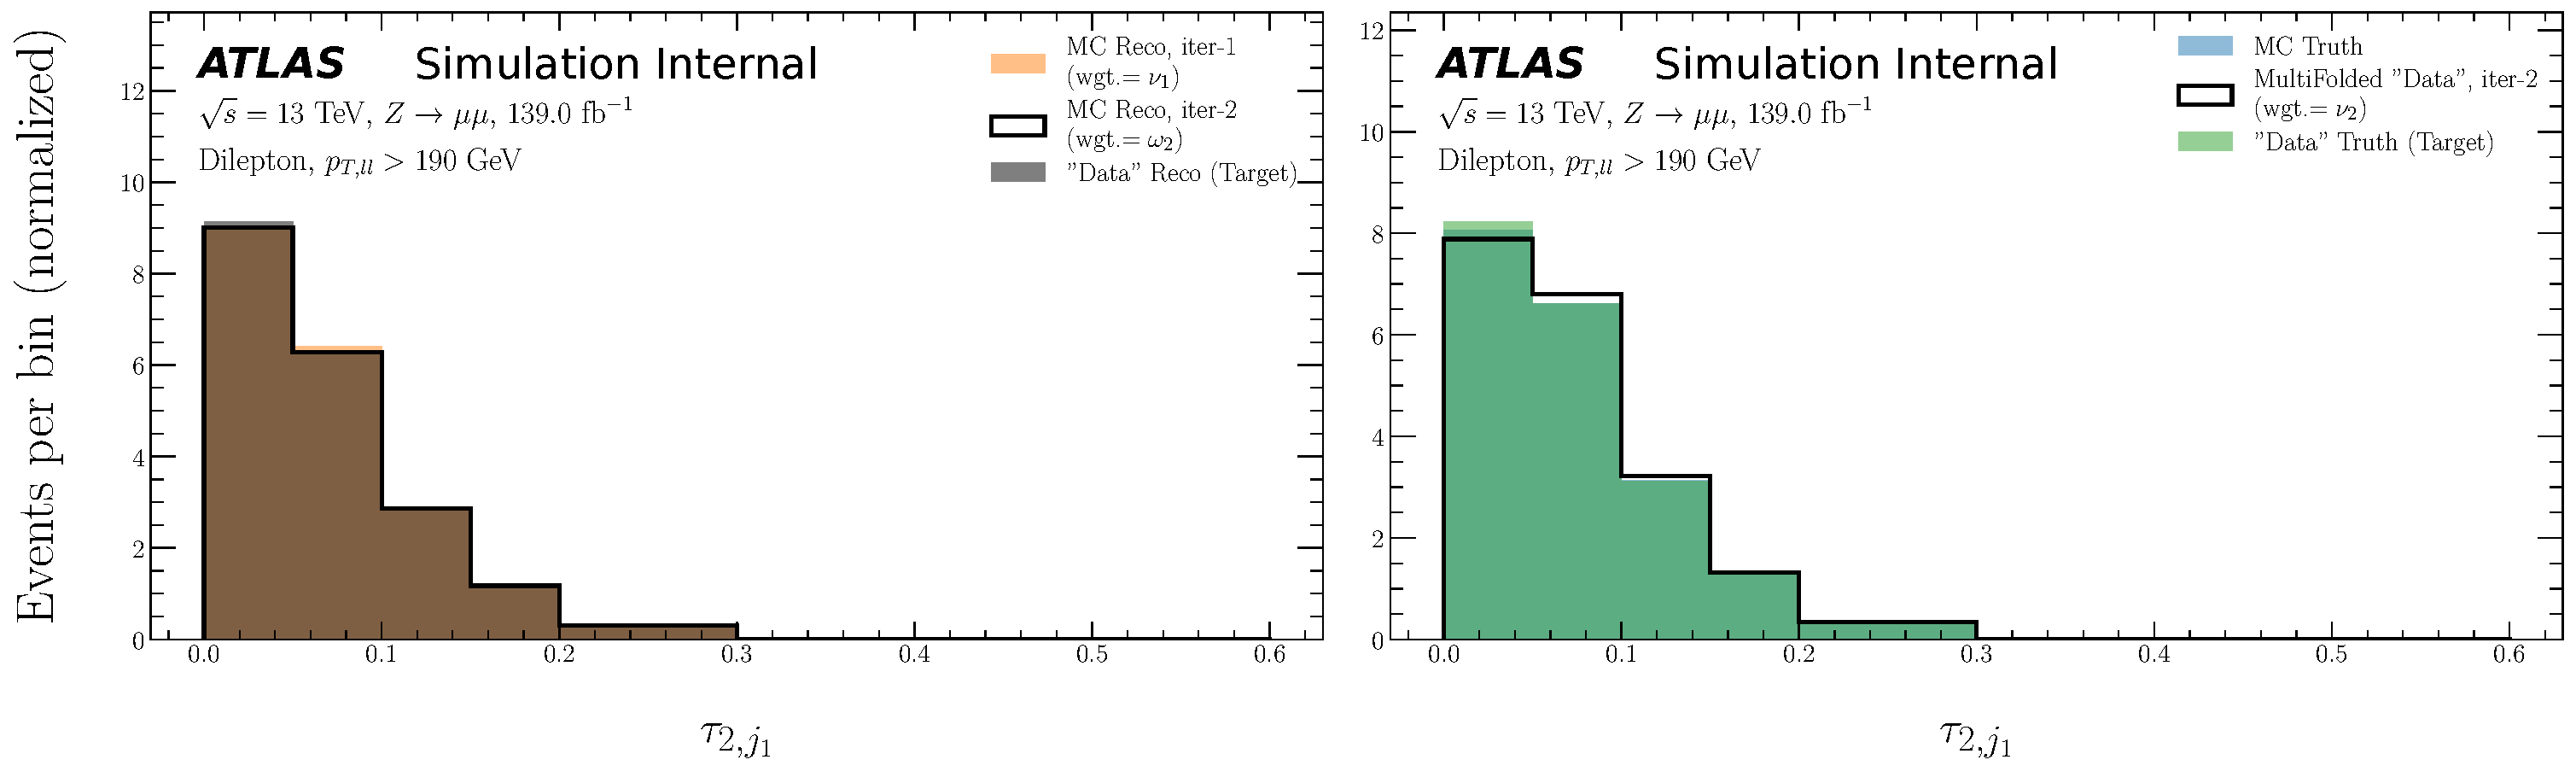
\includegraphics[width=0.85\textwidth]{figures/ATLASOmniFold-StressTest/ATLASOmniFold-StressTestC/MultiFold/tau2_trackj1/ATLASOmniFold-StressTestC-MultiFold-tau2_trackj1-Iteration02}}
\phantomcaption 
\end{figure}

\begin{figure}[h!]
\centering
\ContinuedFloat
\subfloat[After 3 iterations]{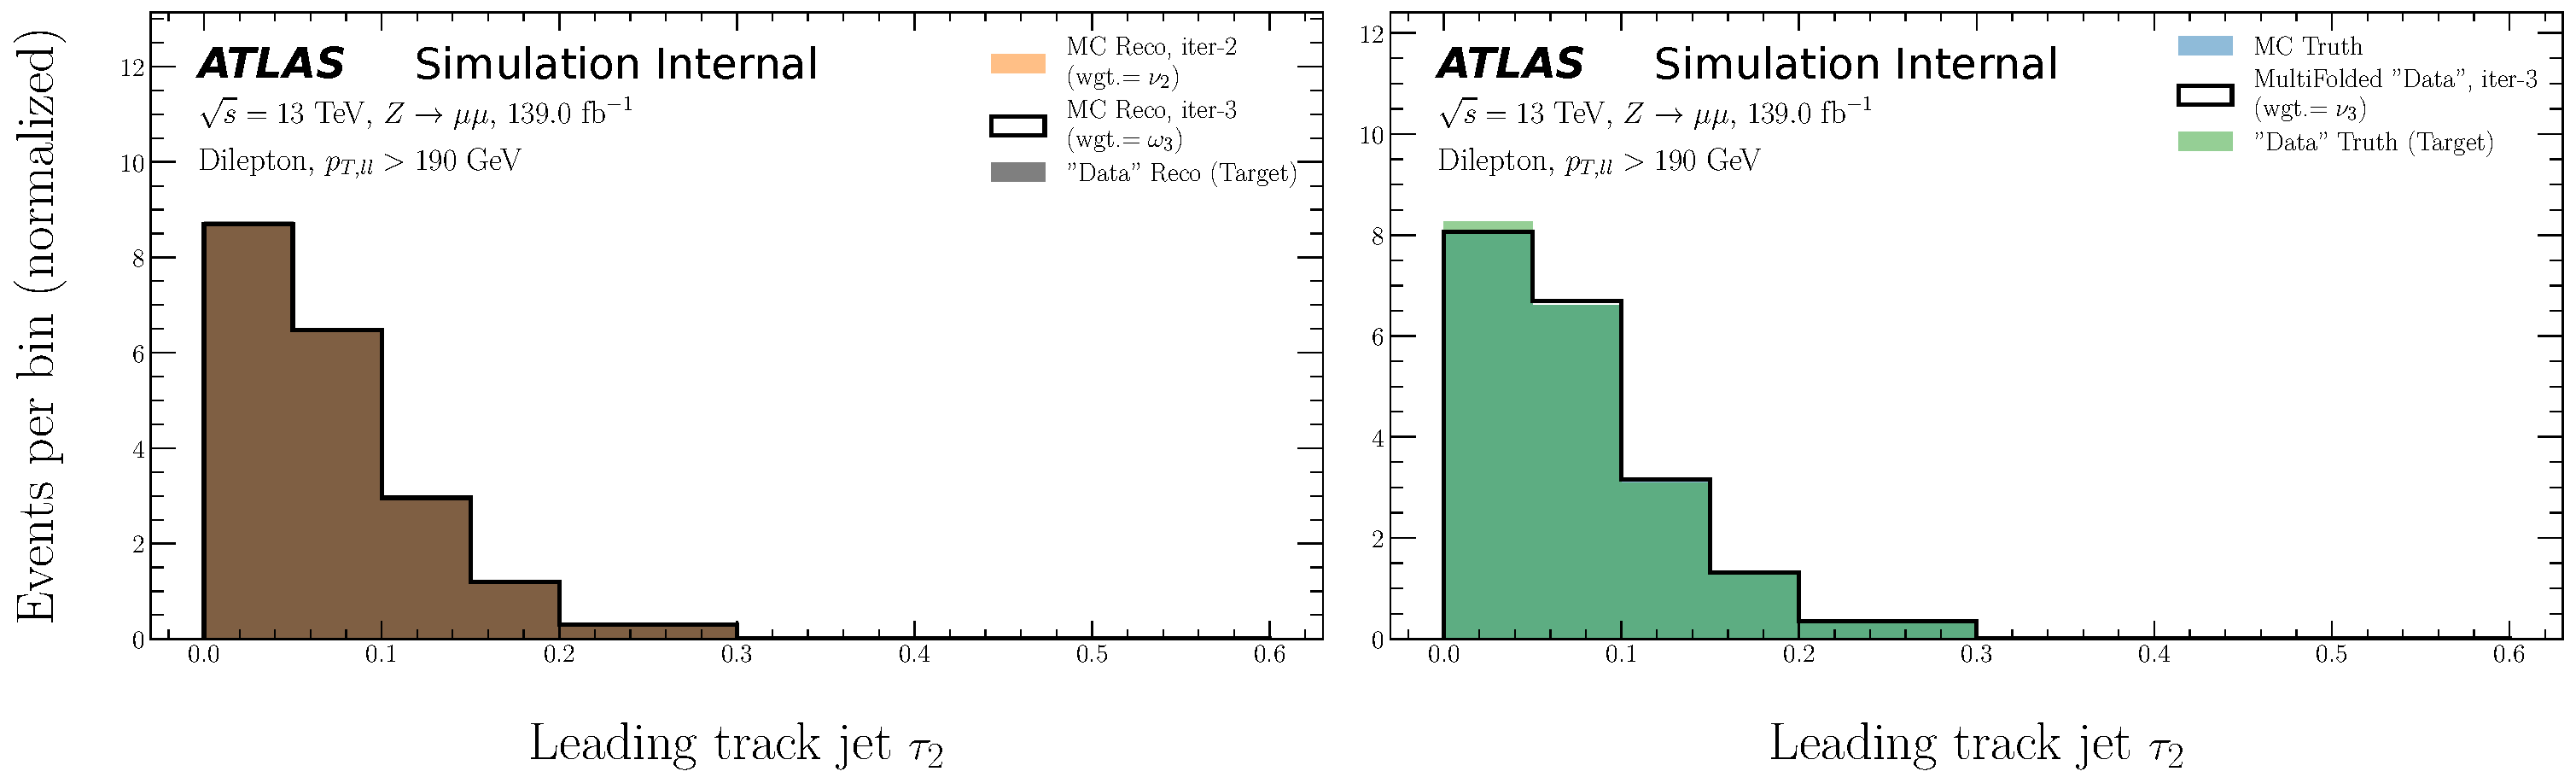
\includegraphics[width=0.85\textwidth]{figures/ATLASOmniFold-StressTest/ATLASOmniFold-StressTestC/MultiFold/tau2_trackj1/ATLASOmniFold-StressTestC-MultiFold-tau2_trackj1-Iteration03}}\\
\subfloat[After 4 iterations]{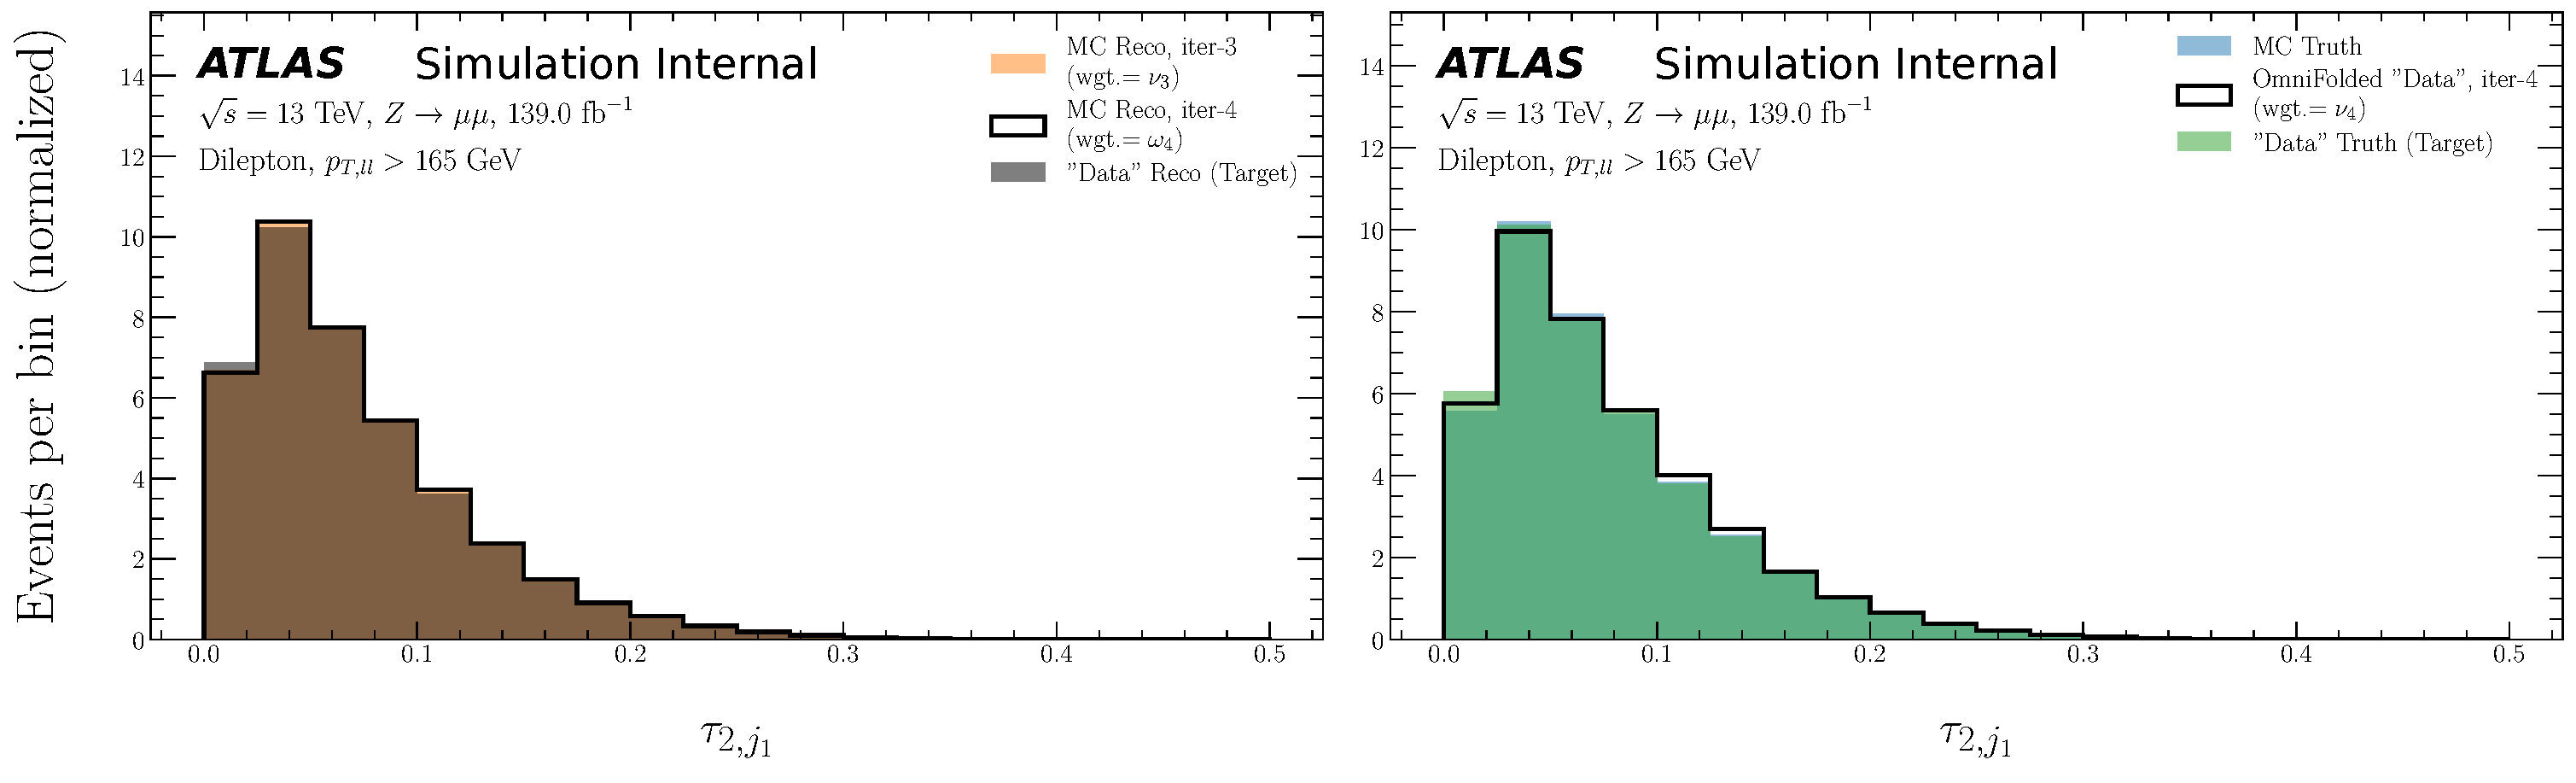
\includegraphics[width=0.85\textwidth]{figures/ATLASOmniFold-StressTest/ATLASOmniFold-StressTestC/MultiFold/tau2_trackj1/ATLASOmniFold-StressTestC-MultiFold-tau2_trackj1-Iteration04}}\\
\subfloat[After 5 iterations]{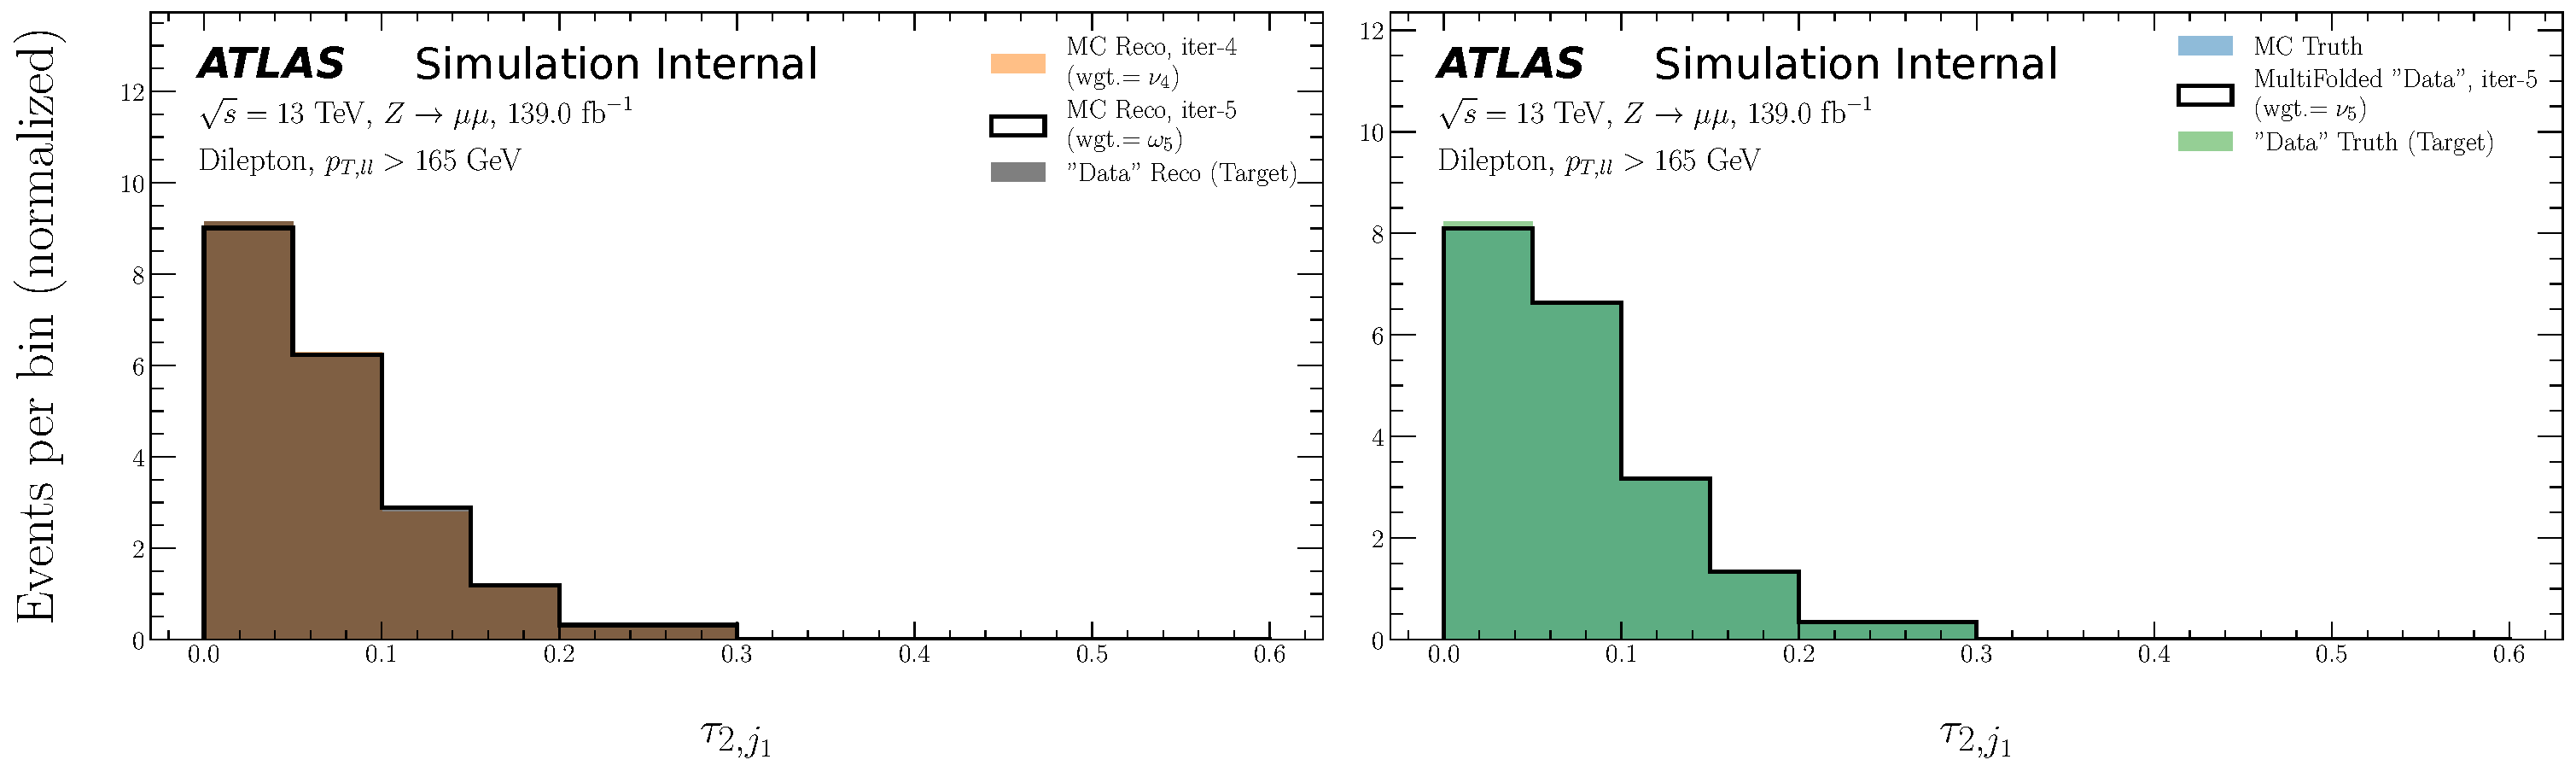
\includegraphics[width=0.85\textwidth]{figures/ATLASOmniFold-StressTest/ATLASOmniFold-StressTestC/MultiFold/tau2_trackj1/ATLASOmniFold-StressTestC-MultiFold-tau2_trackj1-Iteration05}}\\
\subfloat[After 6 iterations]{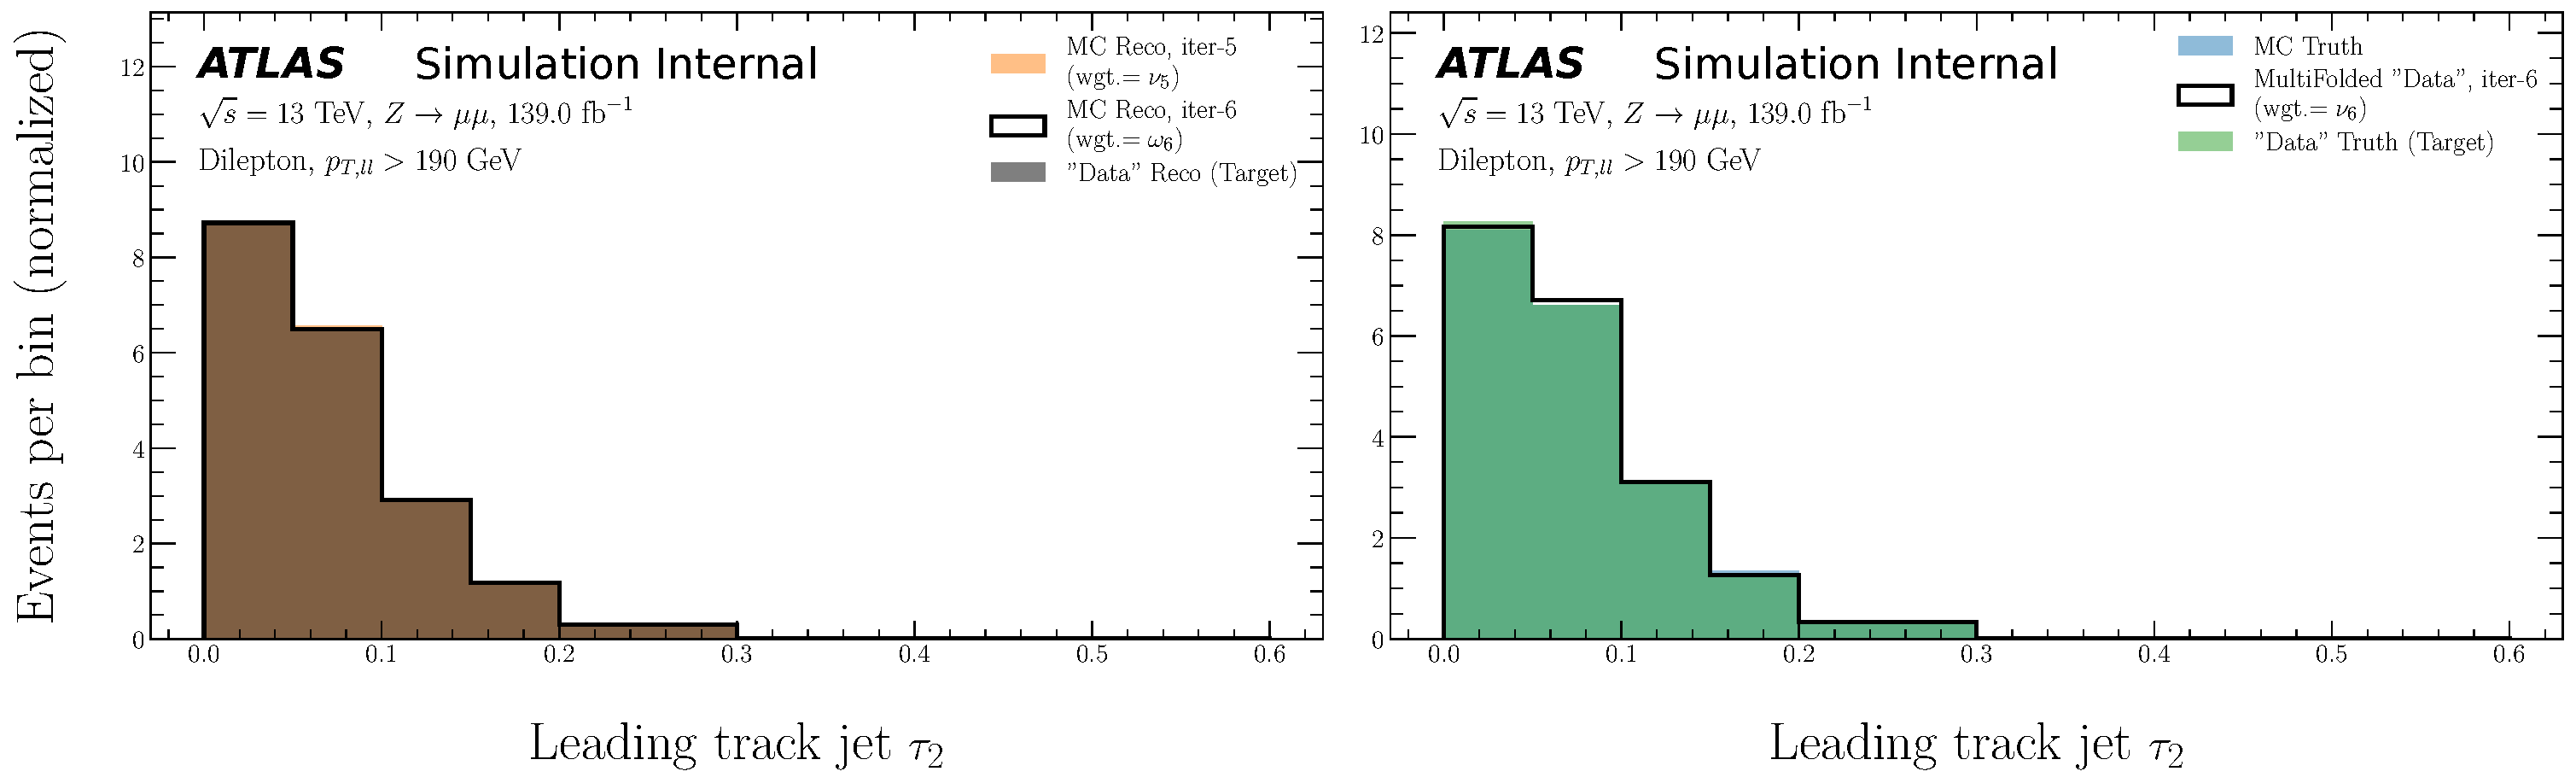
\includegraphics[width=0.85\textwidth]{figures/ATLASOmniFold-StressTest/ATLASOmniFold-StressTestC/MultiFold/tau2_trackj1/ATLASOmniFold-StressTestC-MultiFold-tau2_trackj1-Iteration06}}
\caption{MultiFolding Sherpa with Pythia for the leading track jet $\tau_2$.}
\label{fig:stressc_tau2_trackj1Multi}
\end{figure}

\begin{figure}[h!]
\centering
\subfloat[Input histograms]{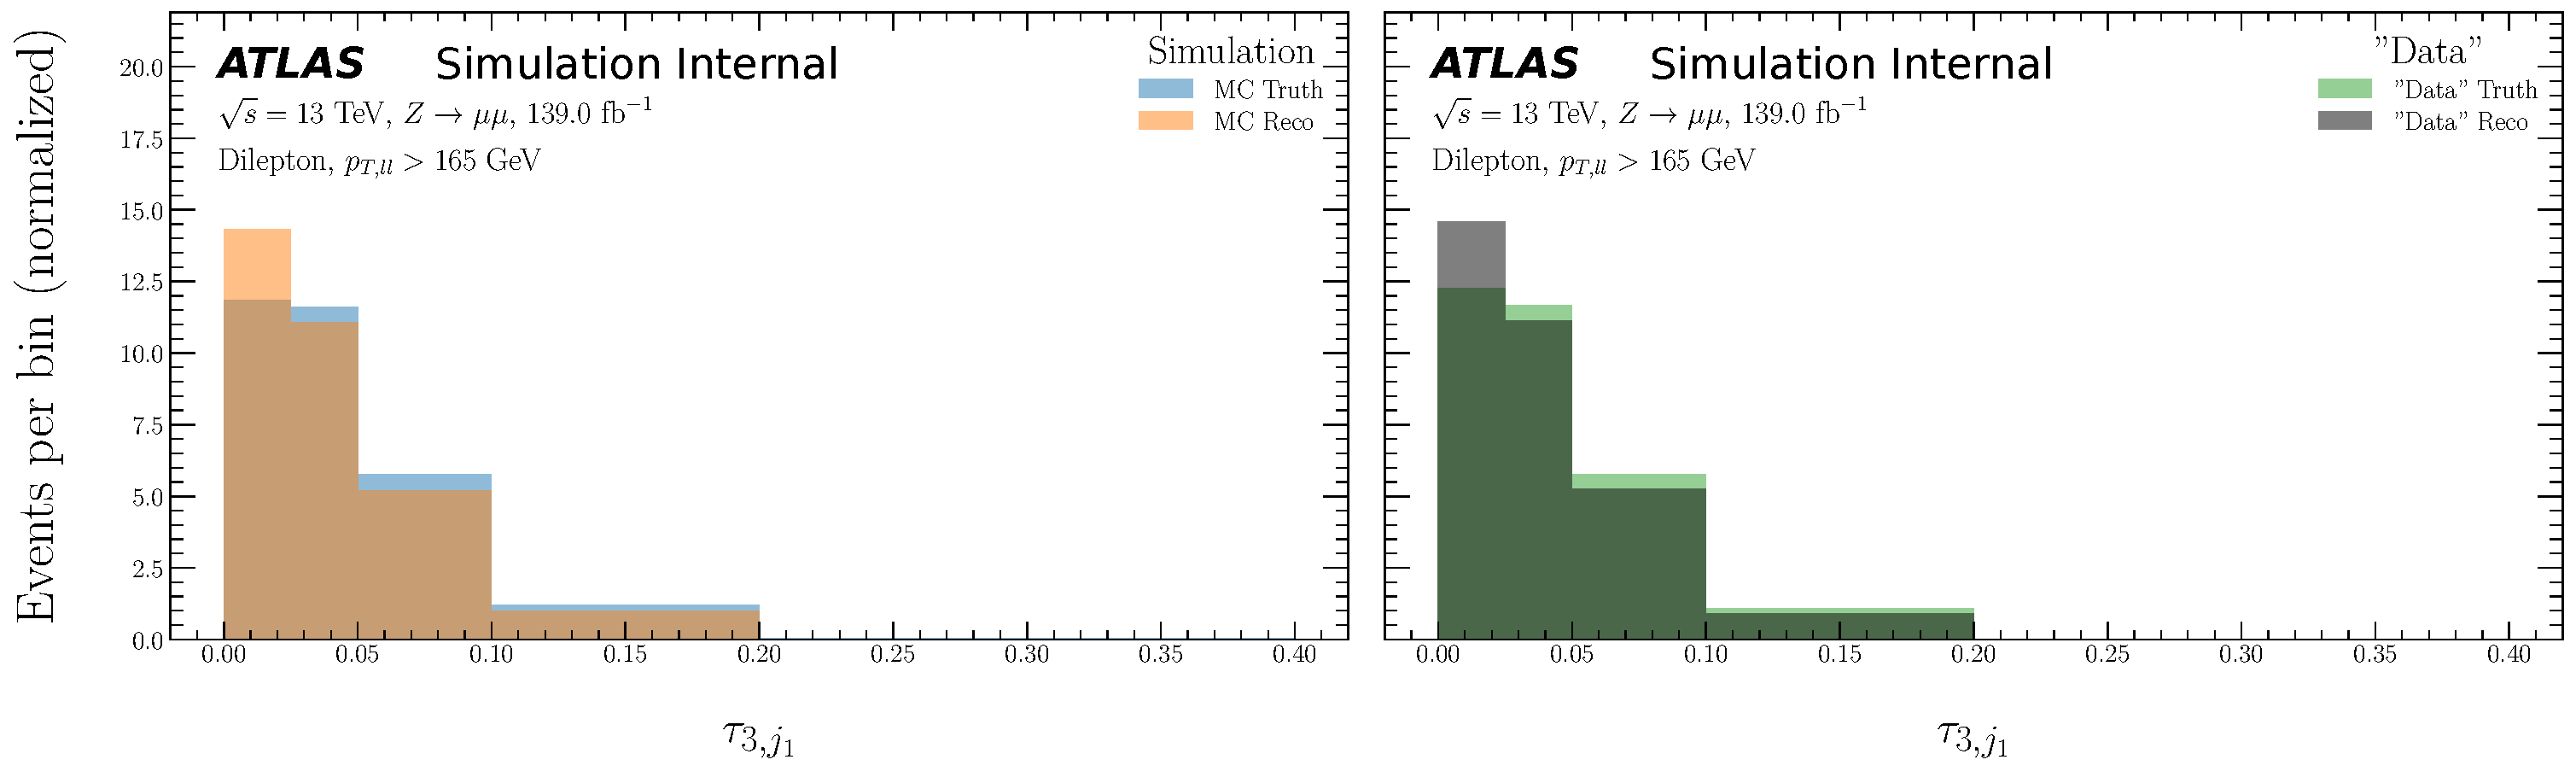
\includegraphics[width=0.85\textwidth]{figures/ATLASOmniFold-StressTest/ATLASOmniFold-StressTestC/MultiFold/tau3_trackj1/ATLASOmniFold-StressTestC-MultiFold-tau3_trackj1-Distributions}}\\
\subfloat[After 1 iteration]{\includegraphics[width=0.85\textwidth]{figures/ATLASOmniFold-StressTest/ATLASOmniFold-StressTestC/MultiFold/tau3_trackj1/ATLASOmniFold-StressTestC-MultiFold-tau3_trackj1-Iteration01}}\\
\subfloat[After 2 iterations]{\includegraphics[width=0.85\textwidth]{figures/ATLASOmniFold-StressTest/ATLASOmniFold-StressTestC/MultiFold/tau3_trackj1/ATLASOmniFold-StressTestC-MultiFold-tau3_trackj1-Iteration02}}
\phantomcaption 
\end{figure}

\begin{figure}[h!]
\centering
\ContinuedFloat
\subfloat[After 3 iterations]{\includegraphics[width=0.85\textwidth]{figures/ATLASOmniFold-StressTest/ATLASOmniFold-StressTestC/MultiFold/tau3_trackj1/ATLASOmniFold-StressTestC-MultiFold-tau3_trackj1-Iteration03}}\\
\subfloat[After 4 iterations]{\includegraphics[width=0.85\textwidth]{figures/ATLASOmniFold-StressTest/ATLASOmniFold-StressTestC/MultiFold/tau3_trackj1/ATLASOmniFold-StressTestC-MultiFold-tau3_trackj1-Iteration04}}\\
\subfloat[After 5 iterations]{\includegraphics[width=0.85\textwidth]{figures/ATLASOmniFold-StressTest/ATLASOmniFold-StressTestC/MultiFold/tau3_trackj1/ATLASOmniFold-StressTestC-MultiFold-tau3_trackj1-Iteration05}}\\
\subfloat[After 6 iterations]{\includegraphics[width=0.85\textwidth]{figures/ATLASOmniFold-StressTest/ATLASOmniFold-StressTestC/MultiFold/tau3_trackj1/ATLASOmniFold-StressTestC-MultiFold-tau3_trackj1-Iteration06}}
\caption{MultiFolding Sherpa with Pythia for the leading track jet $\tau_3$.}
\label{fig:stressc_tau3_trackj1Multi}
\end{figure}

%%%

\begin{figure}[h!]
\centering
\subfloat[Input histograms]{\includegraphics[width=0.85\textwidth]{figures/ATLASOmniFold-StressTest/ATLASOmniFold-StressTestC/MultiFold/m_trackj2/ATLASOmniFold-StressTestC-MultiFold-m_trackj2-Distributions}}\\
\subfloat[After 1 iteration]{\includegraphics[width=0.85\textwidth]{figures/ATLASOmniFold-StressTest/ATLASOmniFold-StressTestC/MultiFold/m_trackj2/ATLASOmniFold-StressTestC-MultiFold-m_trackj2-Iteration01}}\\
\subfloat[After 2 iterations]{\includegraphics[width=0.85\textwidth]{figures/ATLASOmniFold-StressTest/ATLASOmniFold-StressTestC/MultiFold/m_trackj2/ATLASOmniFold-StressTestC-MultiFold-m_trackj2-Iteration02}}
\phantomcaption 
\end{figure}

\begin{figure}[h!]
\centering
\ContinuedFloat
\subfloat[After 3 iterations]{\includegraphics[width=0.85\textwidth]{figures/ATLASOmniFold-StressTest/ATLASOmniFold-StressTestC/MultiFold/m_trackj2/ATLASOmniFold-StressTestC-MultiFold-m_trackj2-Iteration03}}\\
\subfloat[After 4 iterations]{\includegraphics[width=0.85\textwidth]{figures/ATLASOmniFold-StressTest/ATLASOmniFold-StressTestC/MultiFold/m_trackj2/ATLASOmniFold-StressTestC-MultiFold-m_trackj2-Iteration04}}\\
\subfloat[After 5 iterations]{\includegraphics[width=0.85\textwidth]{figures/ATLASOmniFold-StressTest/ATLASOmniFold-StressTestC/MultiFold/m_trackj2/ATLASOmniFold-StressTestC-MultiFold-m_trackj2-Iteration05}}\\
\subfloat[After 6 iterations]{\includegraphics[width=0.85\textwidth]{figures/ATLASOmniFold-StressTest/ATLASOmniFold-StressTestC/MultiFold/m_trackj2/ATLASOmniFold-StressTestC-MultiFold-m_trackj2-Iteration06}}
\caption{MultiFolding Sherpa with Pythia for the subleading track jet mass.}
\label{fig:stressc_massMulti}
\end{figure}

\begin{figure}[h!]
\centering
\subfloat[Input histograms]{\includegraphics[width=0.85\textwidth]{figures/ATLASOmniFold-StressTest/ATLASOmniFold-StressTestC/MultiFold/Ntracks_trackj2/ATLASOmniFold-StressTestC-MultiFold-Ntracks_trackj2-Distributions}}\\
\subfloat[After 1 iteration]{\includegraphics[width=0.85\textwidth]{figures/ATLASOmniFold-StressTest/ATLASOmniFold-StressTestC/MultiFold/Ntracks_trackj2/ATLASOmniFold-StressTestC-MultiFold-Ntracks_trackj2-Iteration01}}\\
\subfloat[After 2 iterations]{\includegraphics[width=0.85\textwidth]{figures/ATLASOmniFold-StressTest/ATLASOmniFold-StressTestC/MultiFold/Ntracks_trackj2/ATLASOmniFold-StressTestC-MultiFold-Ntracks_trackj2-Iteration02}}
\phantomcaption 
\end{figure}

\begin{figure}[h!]
\centering
\ContinuedFloat
\subfloat[After 3 iterations]{\includegraphics[width=0.85\textwidth]{figures/ATLASOmniFold-StressTest/ATLASOmniFold-StressTestC/MultiFold/Ntracks_trackj2/ATLASOmniFold-StressTestC-MultiFold-Ntracks_trackj2-Iteration03}}\\
\subfloat[After 4 iterations]{\includegraphics[width=0.85\textwidth]{figures/ATLASOmniFold-StressTest/ATLASOmniFold-StressTestC/MultiFold/Ntracks_trackj2/ATLASOmniFold-StressTestC-MultiFold-Ntracks_trackj2-Iteration04}}\\
\subfloat[After 5 iterations]{\includegraphics[width=0.85\textwidth]{figures/ATLASOmniFold-StressTest/ATLASOmniFold-StressTestC/MultiFold/Ntracks_trackj2/ATLASOmniFold-StressTestC-MultiFold-Ntracks_trackj2-Iteration05}}\\
\subfloat[After 6 iterations]{\includegraphics[width=0.85\textwidth]{figures/ATLASOmniFold-StressTest/ATLASOmniFold-StressTestC/MultiFold/Ntracks_trackj2/ATLASOmniFold-StressTestC-MultiFold-Ntracks_trackj2-Iteration06}}
\caption{MultiFolding Sherpa with Pythia for the subleading track jet constituent multiplicity.}
\label{fig:stressc_Ntracks_trackj2Multi}
\end{figure}


%%%

\begin{figure}[h!]
\centering
\subfloat[Input histograms]{\includegraphics[width=0.85\textwidth]{figures/ATLASOmniFold-StressTest/ATLASOmniFold-StressTestC/MultiFold/pT_trackj2/ATLASOmniFold-StressTestC-MultiFold-pT_trackj2-Distributions}}\\
\subfloat[After 1 iteration]{\includegraphics[width=0.85\textwidth]{figures/ATLASOmniFold-StressTest/ATLASOmniFold-StressTestC/MultiFold/pT_trackj2/ATLASOmniFold-StressTestC-MultiFold-pT_trackj2-Iteration01}}\\
\subfloat[After 2 iterations]{\includegraphics[width=0.85\textwidth]{figures/ATLASOmniFold-StressTest/ATLASOmniFold-StressTestC/MultiFold/pT_trackj2/ATLASOmniFold-StressTestC-MultiFold-pT_trackj2-Iteration02}}
\phantomcaption 
\end{figure}

\begin{figure}[h!]
\centering
\ContinuedFloat
\subfloat[After 3 iterations]{\includegraphics[width=0.85\textwidth]{figures/ATLASOmniFold-StressTest/ATLASOmniFold-StressTestC/MultiFold/pT_trackj2/ATLASOmniFold-StressTestC-MultiFold-pT_trackj2-Iteration03}}\\
\subfloat[After 4 iterations]{\includegraphics[width=0.85\textwidth]{figures/ATLASOmniFold-StressTest/ATLASOmniFold-StressTestC/MultiFold/pT_trackj2/ATLASOmniFold-StressTestC-MultiFold-pT_trackj2-Iteration04}}\\
\subfloat[After 5 iterations]{\includegraphics[width=0.85\textwidth]{figures/ATLASOmniFold-StressTest/ATLASOmniFold-StressTestC/MultiFold/pT_trackj2/ATLASOmniFold-StressTestC-MultiFold-pT_trackj2-Iteration05}}\\
\subfloat[After 6 iterations]{\includegraphics[width=0.85\textwidth]{figures/ATLASOmniFold-StressTest/ATLASOmniFold-StressTestC/MultiFold/pT_trackj2/ATLASOmniFold-StressTestC-MultiFold-pT_trackj2-Iteration06}}
\caption{MultiFolding Sherpa with Pythia for the subleading track jet $p_T$.}
\label{fig:stressc_pT_trackj2Multi}
\end{figure}

\begin{figure}[h!]
\centering
\subfloat[Input histograms]{\includegraphics[width=0.85\textwidth]{figures/ATLASOmniFold-StressTest/ATLASOmniFold-StressTestC/MultiFold/y_trackj2/ATLASOmniFold-StressTestC-MultiFold-y_trackj2-Distributions}}\\
\subfloat[After 1 iteration]{\includegraphics[width=0.85\textwidth]{figures/ATLASOmniFold-StressTest/ATLASOmniFold-StressTestC/MultiFold/y_trackj2/ATLASOmniFold-StressTestC-MultiFold-y_trackj2-Iteration01}}\\
\subfloat[After 2 iterations]{\includegraphics[width=0.85\textwidth]{figures/ATLASOmniFold-StressTest/ATLASOmniFold-StressTestC/MultiFold/y_trackj2/ATLASOmniFold-StressTestC-MultiFold-y_trackj2-Iteration02}}
\phantomcaption 
\end{figure}

\begin{figure}[h!]
\centering
\ContinuedFloat
\subfloat[After 3 iterations]{\includegraphics[width=0.85\textwidth]{figures/ATLASOmniFold-StressTest/ATLASOmniFold-StressTestC/MultiFold/y_trackj2/ATLASOmniFold-StressTestC-MultiFold-y_trackj2-Iteration03}}\\
\subfloat[After 4 iterations]{\includegraphics[width=0.85\textwidth]{figures/ATLASOmniFold-StressTest/ATLASOmniFold-StressTestC/MultiFold/y_trackj2/ATLASOmniFold-StressTestC-MultiFold-y_trackj2-Iteration04}}\\
\subfloat[After 5 iterations]{\includegraphics[width=0.85\textwidth]{figures/ATLASOmniFold-StressTest/ATLASOmniFold-StressTestC/MultiFold/y_trackj2/ATLASOmniFold-StressTestC-MultiFold-y_trackj2-Iteration05}}\\
\subfloat[After 6 iterations]{\includegraphics[width=0.85\textwidth]{figures/ATLASOmniFold-StressTest/ATLASOmniFold-StressTestC/MultiFold/y_trackj2/ATLASOmniFold-StressTestC-MultiFold-y_trackj2-Iteration06}}
\caption{MultiFolding Sherpa with Pythia for the subleading track jet rapidity.}
\label{fig:stressc_y_trackj2Multi}
\end{figure}

\begin{figure}[h!]
\centering
\subfloat[Input histograms]{\includegraphics[width=0.85\textwidth]{figures/ATLASOmniFold-StressTest/ATLASOmniFold-StressTestC/MultiFold/tau1_trackj2/ATLASOmniFold-StressTestC-MultiFold-tau1_trackj2-Distributions}}\\
\subfloat[After 1 iteration]{\includegraphics[width=0.85\textwidth]{figures/ATLASOmniFold-StressTest/ATLASOmniFold-StressTestC/MultiFold/tau1_trackj2/ATLASOmniFold-StressTestC-MultiFold-tau1_trackj2-Iteration01}}\\
\subfloat[After 2 iterations]{\includegraphics[width=0.85\textwidth]{figures/ATLASOmniFold-StressTest/ATLASOmniFold-StressTestC/MultiFold/tau1_trackj2/ATLASOmniFold-StressTestC-MultiFold-tau1_trackj2-Iteration02}}
\phantomcaption 
\end{figure}

\begin{figure}[h!]
\centering
\ContinuedFloat
\subfloat[After 3 iterations]{\includegraphics[width=0.85\textwidth]{figures/ATLASOmniFold-StressTest/ATLASOmniFold-StressTestC/MultiFold/tau1_trackj2/ATLASOmniFold-StressTestC-MultiFold-tau1_trackj2-Iteration03}}\\
\subfloat[After 4 iterations]{\includegraphics[width=0.85\textwidth]{figures/ATLASOmniFold-StressTest/ATLASOmniFold-StressTestC/MultiFold/tau1_trackj2/ATLASOmniFold-StressTestC-MultiFold-tau1_trackj2-Iteration04}}\\
\subfloat[After 5 iterations]{\includegraphics[width=0.85\textwidth]{figures/ATLASOmniFold-StressTest/ATLASOmniFold-StressTestC/MultiFold/tau1_trackj2/ATLASOmniFold-StressTestC-MultiFold-tau1_trackj2-Iteration05}}\\
\subfloat[After 6 iterations]{\includegraphics[width=0.85\textwidth]{figures/ATLASOmniFold-StressTest/ATLASOmniFold-StressTestC/MultiFold/tau1_trackj2/ATLASOmniFold-StressTestC-MultiFold-tau1_trackj2-Iteration06}}
\caption{MultiFolding Sherpa with Pythia for the subleading track jet $\tau_1$.}
\label{fig:stressc_tau1_trackj2Multi}
\end{figure}

\begin{figure}[h!]
\centering
\subfloat[Input histograms]{\includegraphics[width=0.85\textwidth]{figures/ATLASOmniFold-StressTest/ATLASOmniFold-StressTestC/MultiFold/tau2_trackj2/ATLASOmniFold-StressTestC-MultiFold-tau2_trackj2-Distributions}}\\
\subfloat[After 1 iteration]{\includegraphics[width=0.85\textwidth]{figures/ATLASOmniFold-StressTest/ATLASOmniFold-StressTestC/MultiFold/tau2_trackj2/ATLASOmniFold-StressTestC-MultiFold-tau2_trackj2-Iteration01}}\\
\subfloat[After 2 iterations]{\includegraphics[width=0.85\textwidth]{figures/ATLASOmniFold-StressTest/ATLASOmniFold-StressTestC/MultiFold/tau2_trackj2/ATLASOmniFold-StressTestC-MultiFold-tau2_trackj2-Iteration02}}
\phantomcaption 
\end{figure}

\begin{figure}[h!]
\centering
\ContinuedFloat
\subfloat[After 3 iterations]{\includegraphics[width=0.85\textwidth]{figures/ATLASOmniFold-StressTest/ATLASOmniFold-StressTestC/MultiFold/tau2_trackj2/ATLASOmniFold-StressTestC-MultiFold-tau2_trackj2-Iteration03}}\\
\subfloat[After 4 iterations]{\includegraphics[width=0.85\textwidth]{figures/ATLASOmniFold-StressTest/ATLASOmniFold-StressTestC/MultiFold/tau2_trackj2/ATLASOmniFold-StressTestC-MultiFold-tau2_trackj2-Iteration04}}\\
\subfloat[After 5 iterations]{\includegraphics[width=0.85\textwidth]{figures/ATLASOmniFold-StressTest/ATLASOmniFold-StressTestC/MultiFold/tau2_trackj2/ATLASOmniFold-StressTestC-MultiFold-tau2_trackj2-Iteration05}}\\
\subfloat[After 6 iterations]{\includegraphics[width=0.85\textwidth]{figures/ATLASOmniFold-StressTest/ATLASOmniFold-StressTestC/MultiFold/tau2_trackj2/ATLASOmniFold-StressTestC-MultiFold-tau2_trackj2-Iteration06}}
\caption{MultiFolding Sherpa with Pythia for the subleading track jet $\tau_2$.}
\label{fig:stressc_tau2_trackj2Multi}
\end{figure}

\begin{figure}[h!]
\centering
\subfloat[Input histograms]{\includegraphics[width=0.85\textwidth]{figures/ATLASOmniFold-StressTest/ATLASOmniFold-StressTestC/MultiFold/tau3_trackj2/ATLASOmniFold-StressTestC-MultiFold-tau3_trackj2-Distributions}}\\
\subfloat[After 1 iteration]{\includegraphics[width=0.85\textwidth]{figures/ATLASOmniFold-StressTest/ATLASOmniFold-StressTestC/MultiFold/tau3_trackj2/ATLASOmniFold-StressTestC-MultiFold-tau3_trackj2-Iteration01}}\\
\subfloat[After 2 iterations]{\includegraphics[width=0.85\textwidth]{figures/ATLASOmniFold-StressTest/ATLASOmniFold-StressTestC/MultiFold/tau3_trackj2/ATLASOmniFold-StressTestC-MultiFold-tau3_trackj2-Iteration02}}
\phantomcaption 
\end{figure}

\begin{figure}[h!]
\centering
\ContinuedFloat
\subfloat[After 3 iterations]{\includegraphics[width=0.85\textwidth]{figures/ATLASOmniFold-StressTest/ATLASOmniFold-StressTestC/MultiFold/tau3_trackj2/ATLASOmniFold-StressTestC-MultiFold-tau3_trackj2-Iteration03}}\\
\subfloat[After 4 iterations]{\includegraphics[width=0.85\textwidth]{figures/ATLASOmniFold-StressTest/ATLASOmniFold-StressTestC/MultiFold/tau3_trackj2/ATLASOmniFold-StressTestC-MultiFold-tau3_trackj2-Iteration04}}\\
\subfloat[After 5 iterations]{\includegraphics[width=0.85\textwidth]{figures/ATLASOmniFold-StressTest/ATLASOmniFold-StressTestC/MultiFold/tau3_trackj2/ATLASOmniFold-StressTestC-MultiFold-tau3_trackj2-Iteration05}}\\
\subfloat[After 6 iterations]{\includegraphics[width=0.85\textwidth]{figures/ATLASOmniFold-StressTest/ATLASOmniFold-StressTestC/MultiFold/tau3_trackj2/ATLASOmniFold-StressTestC-MultiFold-tau3_trackj2-Iteration06}}
\caption{MultiFolding Sherpa with Pythia for the subleading track jet $\tau_3$.}
\label{fig:stressc_tau3_trackj2Multi}
\end{figure}

%%%

\begin{figure}[h!]
\centering
\subfloat[Input histograms]{\includegraphics[width=0.85\textwidth]{figures/ATLASOmniFold-StressTest/ATLASOmniFold-StressTestC/MultiFold/pT_ll/ATLASOmniFold-StressTestC-MultiFold-pT_ll-Distributions}}\\
\subfloat[After 1 iteration]{\includegraphics[width=0.85\textwidth]{figures/ATLASOmniFold-StressTest/ATLASOmniFold-StressTestC/MultiFold/pT_ll/ATLASOmniFold-StressTestC-MultiFold-pT_ll-Iteration01}}\\
\subfloat[After 2 iterations]{\includegraphics[width=0.85\textwidth]{figures/ATLASOmniFold-StressTest/ATLASOmniFold-StressTestC/MultiFold/pT_ll/ATLASOmniFold-StressTestC-MultiFold-pT_ll-Iteration02}}
\phantomcaption 
\end{figure}

\begin{figure}[h!]
\centering
\ContinuedFloat
\subfloat[After 3 iterations]{\includegraphics[width=0.85\textwidth]{figures/ATLASOmniFold-StressTest/ATLASOmniFold-StressTestC/MultiFold/pT_ll/ATLASOmniFold-StressTestC-MultiFold-pT_ll-Iteration03}}\\
\subfloat[After 4 iterations]{\includegraphics[width=0.85\textwidth]{figures/ATLASOmniFold-StressTest/ATLASOmniFold-StressTestC/MultiFold/pT_ll/ATLASOmniFold-StressTestC-MultiFold-pT_ll-Iteration04}}\\
\subfloat[After 5 iterations]{\includegraphics[width=0.85\textwidth]{figures/ATLASOmniFold-StressTest/ATLASOmniFold-StressTestC/MultiFold/pT_ll/ATLASOmniFold-StressTestC-MultiFold-pT_ll-Iteration05}}\\
\subfloat[After 6 iterations]{\includegraphics[width=0.85\textwidth]{figures/ATLASOmniFold-StressTest/ATLASOmniFold-StressTestC/MultiFold/pT_ll/ATLASOmniFold-StressTestC-MultiFold-pT_ll-Iteration06}}
\caption{MultiFolding Sherpa with Pythia for $p_{T,ll}$.}
\label{fig:stressc_pT_llMulti}
\end{figure}

\begin{figure}[h!]
\centering
\subfloat[Input histograms]{\includegraphics[width=0.85\textwidth]{figures/ATLASOmniFold-StressTest/ATLASOmniFold-StressTestC/MultiFold/y_ll/ATLASOmniFold-StressTestC-MultiFold-y_ll-Distributions}}\\
\subfloat[After 1 iteration]{\includegraphics[width=0.85\textwidth]{figures/ATLASOmniFold-StressTest/ATLASOmniFold-StressTestC/MultiFold/y_ll/ATLASOmniFold-StressTestC-MultiFold-y_ll-Iteration01}}\\
\subfloat[After 2 iterations]{\includegraphics[width=0.85\textwidth]{figures/ATLASOmniFold-StressTest/ATLASOmniFold-StressTestC/MultiFold/y_ll/ATLASOmniFold-StressTestC-MultiFold-y_ll-Iteration02}}
\phantomcaption 
\end{figure}

\begin{figure}[h!]
\centering
\ContinuedFloat
\subfloat[After 3 iterations]{\includegraphics[width=0.85\textwidth]{figures/ATLASOmniFold-StressTest/ATLASOmniFold-StressTestC/MultiFold/y_ll/ATLASOmniFold-StressTestC-MultiFold-y_ll-Iteration03}}\\
\subfloat[After 4 iterations]{\includegraphics[width=0.85\textwidth]{figures/ATLASOmniFold-StressTest/ATLASOmniFold-StressTestC/MultiFold/y_ll/ATLASOmniFold-StressTestC-MultiFold-y_ll-Iteration04}}\\
\subfloat[After 5 iterations]{\includegraphics[width=0.85\textwidth]{figures/ATLASOmniFold-StressTest/ATLASOmniFold-StressTestC/MultiFold/y_ll/ATLASOmniFold-StressTestC-MultiFold-y_ll-Iteration05}}\\
\subfloat[After 6 iterations]{\includegraphics[width=0.85\textwidth]{figures/ATLASOmniFold-StressTest/ATLASOmniFold-StressTestC/MultiFold/y_ll/ATLASOmniFold-StressTestC-MultiFold-y_ll-Iteration06}}
\caption{MultiFolding Sherpa with Pythia for $y_{ll}$.}
\label{fig:stressc_y_llMulti}
\end{figure}
